\documentclass[10pt]{report}
\usepackage[utf8]{inputenc}

\usepackage{graphicx}
\usepackage{geometry}
\usepackage{enumitem}
\usepackage{hyperref}
\usepackage{colortbl}
\usepackage{array}
\usepackage{float}
\usepackage{tabularx}
\usepackage{longtable}
\usepackage{listing}
\usepackage{listings}
\usepackage{alloy}
\usepackage{xcolor}

\hypersetup{
    colorlinks=true,
    linkcolor=blue,
    filecolor=magenta,      
    urlcolor=cyan,
    pdftitle={Requirement Analysis and Specification Document},}

\graphicspath{ {Images/} }
\geometry{a4paper, margin=100px}

\title{Requirement Analysis and Specification Document}
% https://github.com/AndreaPrati98/MaccarronePellizzerPrati
\author{Maccarrone Salvatore,   Pellizzer Massimiliano,   Prati Andrea}
\date{\today}

\begin{document}

% Title Page
% ----------------------------------------------------------------------------------------------------
% Title Page
% ----------------------------------------------------------------------------------------------------
\begin{titlepage}
    \begin{figure}[t]
        \centering
        
\includegraphics[width=250px]{/PolimiLogo}
    \end{figure}
    \begin{centering}
       \maketitle
    \end{centering}
\end{titlepage}

% ----------------------------------------------------------------------------------------------------
% ----------------------------------------------------------------------------------------------------

\tableofcontents

\chapter{Introduction}
Agriculture plays a pivotal role in India’s economy. Climate change continues to be a real and potent threat to the agriculture sector, which will impact everything from productivity to livelihoods across food and farm systems and is predicted to result in a 4\%-26\% loss in net farm income towards the end of the century. This calls for a revamp of the entire mechanism that brings food from farms to our plates. The COVID-19 pandemic has greatly highlighted the massive disruption caused in food supply chains exposing the vulnerabilities of marginalized communities, small holder farmers and the importance of building resilient food systems. It has become even more important now that we develop and adopt innovative methodologies and technologies that can help bolster countries against food supply shocks and challenges.

    \section{Purpose}
    Telangana’s government wants to design, develop and demonstrate anticipatory governance models for food systems using digital public goods and community-centric approaches to strengthen data-driven policy making in the state. This will require the involvement of multiple stakeholders, from normal citizens to policy makers, farmers, market analysts, agronomists and so on. \\ \\
    In the first place, Telangana wants to partner with IT providers with the aim of acquiring and combining: \\ 
    Data concerning meteorological short-term and long-term forecasts. Telangana already collects and makes available such data (see https://www.tsdps.telangana.gov.in/aws.jsp).
    \begin{itemize}
    \item Information provided by the farmers about their production (types of products, produced amount per product). 
    \item Information obtained by the water irrigation system concerning the amount of water used by each farmer. 
    \item Information obtained by sensors deployed on the territory and measuring the humidity of soil.
    \item Information obtained by the governmental agronomists who periodically visit the farms in their areas.
    \end{itemize}
    Acquiring and combining such data, DREAM will support the work of three types of actors: policy makers, farmers, and agronomists. In the following we describe the goals summed up.

    \subsection{Goals}
    \subsubsection{G1 - Data-Driven approach}
    \emph{DREAM} will be able to fetch data from different databases. Then, DREAM will be able to collect, analyze and perform inference on this data in order to extract new knowledge that will be at the service of different \emph{DREAM}’s users.
    \subsubsection{G2 - Help policy makers to implement better policies which will make Telangana’s agriculture better}
    \emph{DREAM} will allow policy makers to see real time data regarding Telangana and Telangana’s farms. In particular they will be able to see which farms are performing well and which farms are performing poorly. Moreover, they will be able to understand which steering initiatives are working and which not.
    \subsubsection{G3 - Help farmers to become weather resilient and increase their production}
    \emph{DREAM} will allow farmers to see statistics regarding their farms. Moreover, \emph{DREAM} will provide to them personalized suggestions based on the data regarding their farm and on the data regarding farms that are doing particularly well in similar environments.
    \subsubsection{G4 - Facilitate and make systematic the communication between farmers and agronomists}
    \emph{DREAM} will make communications between agronomists and farmers easy and stable. In fact, \emph{DREAM} will allow farmers to chat with agronomists in just a few clicks. Moreover they will be able to request agronomists to visit them when they are facing complex problems.
    Agronomists, instead, will be able to access real time data regarding farms they are responsible for, and therefore they will be able to see which farms are performing well and which farms are performing poorly. Based on this knowledge, agronomists will be able to decide how much and when to visit each farm, and to send periodical reports to policy makers regarding how the farms (they are responsible for) are doing.
    \subsubsection{G5 - Create a network of farmers}
    Through \emph{DREAM}, farmers will be able to communicate between each other in order to exchange best practices and advice.
    \section{Scope}
    The problem that Telangana is facing concerns the world of agriculture, and it has a very important weight on the lives of many people who, due to various impediments mentioned in the previous section, need a platform that can support them and allow those who create support initiatives to do the work in the most scientific way possible, keeping track of how is all going on without losing information. \\ \\
    To reach this goal, called "data-driven approach" it was necessary to think at an entire platform. In particular, this platform can be seen as divided into three categories:
    \begin{itemize}
        \item Data: users must be able to easily interact with the data to which they have the right to access. They are offered different views and aggregations with respect to this data. The available data can include weather forecasts, the state and composition of the land of an area of Telangana, the water irrigation system (the amount of water used), and the initiatives taken by other farmers who have distinguished themselves for being productive considering the conditions in which they were found (positive and negative deviance). Other types of data are described in the remainder of the document.
        \item Community: users are able to communicate via two communication channels within the system, one is the Forum and the other is the Chat System that will allow Farmers and Agronomists to talk to each other to exchange advice and clarifications.
        \item Management: users can organize physical visits between Agronomists and Farmers directly in the app.
    \end{itemize}
    The processing of data and their analysis was not the focus for the drafting of this document. In fact, the first goal was to think about how to develop the platform as a whole. The choice on which criteria to calculate the Farmer's performance (i.e. their deviance, positive or negative) will be made thanks to the collaboration with expert agronomists who will provide all the knowledge to be able to create and study intelligent models using special tools such as, TensorFlow, a framework for processing data. \\
    Moreover, the system will interface itself with different databases maintained and managed by third parties. How the data are inserted or managed in those databases is not one of the concern of the system described in this document.
        \subsection{Phenomena}
            \subsubsection{World Phenomena}
                \begin{itemize}%[margin=5px]
                    \item [$W01$] The farmer weighs the crop
                    \item [$W02$] Physical event that the farmer considers important to report happens
                    \item [$W03$] The farmer faces a problem concerning their farm
                    \item [$W04$] The agronomist misses an appointment
                    \item [$W05$] The agronomist goes to the farmer
                    \item [$W06$] The agronomist takes measures 
                    \item [$W07$] The agronomist assists the farmer while he is in visit to their farm
                    \item [$W08$] The farmer open a chat 
                \end{itemize}
            \subsubsection{Shared Phenomena}
                \begin{itemize}%[margin=5px]
                        \item [$S01$] Registration of the user (World Controlled)
                        \item [$S02$] Login of the user (World Controlled)
                        \item [$S03$] The user queries the system (World Controlled)
                        \item [$S04$] The system shows data to the user (Machine Controlled)
                        \item [$S05$] The user queries the system to retrieve relevant data (World Controlled)
                        \item [$S06$] The system shows agronomists the list of farmers they have to manage (Machine Controlled)
                        \item [$S07$] The farmer inserts data concerning their production (World Controlled)
                        \item [$S08$] The system confirms the success of an operation to the user (Machine Controlled)
                        \item [$S09$] The farmer open a ticket in order to have a chat with an agronomist (World Controlled)
                        \item [$S10$] The system shows an agronomist the list of their currently open chats (Machine Controlled)
                        \item [$S11$] The system shows agronomists the list of chat requests to be managed (Machine Controlled)
                        \item [$S12$] The agronomist accepts a chat request (World Controlled)
                        \item [$S13$] The agronomist closes a chat (World Controlled)
                        \item [$S14$] The farmer interacts with the system’s forum (World Controlled)
                        \item [$S15$] The agronomist schedules an appointment in order to visit a farm (World Controlled)
                        \item [$S16$] The agronomist cancels an appointment from the schedule (World Controlled)
                        \item [$S17$] The agronomist confirms the scheduled appointment done during the day (World Controlled)
                        \item [$S18$] The agronomist inserts a report and other data regarding the appointment done during the day (World Controlled)
                        \item [$S20$] The agronomist get notified
                        \item [$S21$] The farmer get notified
                    \end{itemize}
            \subsubsection{Machine Phenomena}
                \begin{itemize}%[margin=5px]
                    \item [$M01$] The system periodically fetches data from its sources
                    \item [$M02$] The system aggregates and filters data
                    \item [$M03$] The system validates data and stores it
                    \item [$M04$] The system updates the agronomist’s schedule
                    \item [$M05$] The system check the references of the agronomist
                    \item [$M06$] The system checks credentials of the user
                    \item [$M07$] The system generates the list of farmer associated to each agronomist
                    \item [$M08$] The system orders the list of farmers associated to each agronomist by priority
                    \item [$M09$] The system keeps updated the priority of farmers inside their list
                    \item [$M10$] The system removes a chat request from the list and adds a new entry in the list of open chats managed by an agronomists
                    \item [$M11$] The system removes the chat from the list of open chats of the agronomist that taken it into account
                    \item [$M12$] The system synchronizes lists shared between agronomists working on the same area
                    \item [$M13$] The system keeps track of the appointment missed by agronomists
                    \item [$M14$] The system generates personalised suggestions based on historical data to be delivered to the farmer
                \end{itemize}
    \section{Definitions, Acronyms, Abbreviations}
    \subsection{Definitions}
    \emph{Agronomist's schedule} $\rightarrow$ The schedule of an agronomist is a list of planned activities or things to be done showing the times or dates when they are intended to happen or be done. In particular, in this case, the activities are the planned visits to the various farms.
    \\ \\
    \emph{Area} $\rightarrow$ The word "area" indicates a disjoint partition of Telangana. In fact, Telengana is partitioned in several disjoint areas, and to each area are associated both farmers and agronomists, in such a way that:
    \begin{itemize}
        \item Each area can have one or more farmers and one or more agronomists
        \item Each farmer is associated to one and only one area
        \item Each agronomist is associated to one and only one area
    \end{itemize}
    \emph{Chat} $\rightarrow$ A chat is a virtual space that, after it has opened, allows one agronomist and one farmer to discuss with each other.
    \\ \\
    \emph{Data Summary} $\rightarrow$ A data summary is an aggregation of data fetched by various databases, which gives a certain data view of a subject (e.g. a farm or an area).
    \\ \\
    \emph{Data View} $\rightarrow$ A data view is a selection of data fetched by the various databases, regarding a specific aspect (e.g. humidity of soil, water irrigation data) of the subject (e.g. a farm or an area of Telangana).
    \\ \\
    \emph{Priority} $\rightarrow$ The term "priority", when used referring to the list of farms, indicates that the list of farms is sorted taking into account:
    \begin{itemize}
        \item The number of times the farm has already been visited during the year
        \item How well or bad the farm is performing
        \item Possible requests of help done by the farmer
    \end{itemize}
    These metrics define what is referred to as priority.
    \\ \\
    \emph{Relevant data} $\rightarrow$ The term "relevant data" indicates data regarding:
    \begin{itemize}
        \item Data concerning meteorological short-term and long-term forecasts
        \item Information provided by the farmers about their production
        \item Information obtained by the water irrigation system concerning the amount of water used by each farmer
        \item Information obtained by sensors deployed on the territory and measuring the humidity of soil
        \item Information obtained by the governmental agronomists who periodically visit the farms in their areas
    \end{itemize}
    \emph{Report} $\rightarrow$ When an agronomist visits a farm they must write (and insert into the system) a summary of what they have suggested to the farmer, which problems they have detected, and everything they think could be relevant in order to understand why the farmer is performing well or why the farmer is performing poorly. This summary is indicated by the word “report”. The purpose of the report is to keep track of the history of every farm.
    \\ \\
    \emph{Ticket (or Chat Request)} $\rightarrow$ Whenever a farmer wants to have a chat with an agronomist they have to open a ticket. A ticket, thus, is a request to have a chat.
    \\ \\
    \emph{Open a ticket} $\rightarrow$ Open a ticket indicates the action, performed by the farmer, of asking an agronomist to have a chat.
    \\ \\
    \emph{Managed ticket} $\rightarrow$ A managed ticket is a chat request accepted by an agronomist.
    \\ \\
    \emph{Not manged ticket} $\rightarrow$ A ticket that is not managed is a chat request not accepted by any agronomist yet.
    \\ \\
    \emph{Users} $\rightarrow$ The users of the system are: farmers, agronomists and policy makers. Whenever the word "users" is used, it indicates both agronomists, farmers and policy makers.
    \\ \\
    \emph{Visit} $\rightarrow$ In order to help farmers, agronomists can reach the farm of the farmer physically. A visit, therefore, is the action, performed by an agronomist, of physically reaching a farmer's farm.
    \\ \\
    \emph{Booking a visit} $\rightarrow$ To book a visit means reaching an agreement between a farmer and an agronomist on when the agronomist should visit the farm.
    \\ \\
    \emph{Booked visit} $\rightarrow$ A booked visit is a visit that has been scheduled by the agronomist in accordance with the farmer
    \subsection{Acronyms}
    \emph{API} $\rightarrow$ Application Programming Interface, it indicates on demand procedure which supply a specific task.\\ \\
    \emph{BPMN} $\rightarrow$ Business Process Model and Notation, it is a graphical representation for specifying business processes in a business process model.\\ \\
    \emph{DBMS} $\rightarrow$ Data Base Management System, it is an interface between the end user and the database, simultaneously managing the data, the database engine, and the database schema in order to facilitate the organization and manipulation of data.\\ \\
    \emph{DREAM} $\rightarrow$ Data-Drive Predictive Farming in Telengana, is the name software to be developed, described in this document.
    \section{Revision History}
    \begin{itemize}
        \item December 23, 2021: version 1.0 (first release)
    \end{itemize}
    \section{Reference Documents}
    \emph{Reference book} $\rightarrow$ Hans Van Vilet - Software Engineering: Principles and Practice
    \\ \\
    \emph{Alloy official documentation} $\rightarrow$ https://alloytools.org/documentation.html
    \\ \\
    \emph{UML official specification} $\rightarrow$ https://www.omg.org/spec/UML/
    \\ \\
    \emph{BPMN official specification} $\rightarrow$ https://www.omg.org/spec/BPMN/2.0/
    \\ \\
    \emph{Paper} $\rightarrow$ Jackson and Zave: the world and the machine\\ \\
    \emph{Github} $\rightarrow$ https://github.com/UNDP-India/Data4Policy\\ (All the reference written on this repository are reference that we considered as well)
    \section{Document Structure}
    \begin{itemize}
        \item \textbf{Section 1: Introduction}\\
        This section offers a brief overview of the problem, required functionalities and the reference used in order to write this document.\\
        It also contains the list of definitions, acronyms and abbreviations that could be found in this document.\\
        \item \textbf{Section 2: Overall Description}\\
        This section offers the overall organization of the system, the possible scenarios that this application covers and the description of the most important functions that needs to be present in the application.\\
        Here is also possible to find the domain assumptions under which the system works. The actors who use the application are described as well, this way it's easier to identify the type of user the app is designed for.
        \item \textbf{Section 3: Specific Requirements}\\
        This section is the most technical, there is a more precise description of each single important use case. It also explains, through the mapping \textit{goal-assumptions-requirements}, how each functionalities is necessary to reach each goal requested by the client.\\
        It's also possible to understand the hardware and constraints and the attribute needed in the system (reliability, availability, security and so on).
        \item \textbf{Section 4: Formal Analysis through Alloy} \\
        In section number 4 of this document a formal description of the system is found. The Alloy language is used to reach the description (it has been referenced in the section 1) and each simulation done is commented.
        \item \textbf{Section 5: Effort spent} \\
        In the last section of this document is presented the number of hours spent per each person of the group. We decided to include also a "Thought process" section, in order to describe the steps we went trough in order to write this document and why we focused our energies into some details instead of others.
    \end{itemize}

\chapter{Overall Description}
\section{Product Perspective}
The following section contains the UML class diagram of the application and a list of meaningful scenarios where our system can be used.\\ Notice that a further discussion on the implementation details will be covered in the design document.\\ Furthermore, in the list of meaningful scenarios, we highlighted the correlation with the associated use cases, that are thoroughly described in section 3.3.

\subsection{Class diagram}
Here we include the class diagram, in order to show the structure of the system. \\
We structured the system with three type of users, as requested by the assignment, they are all an extension of the class \textbf{User}, which is the one that can interact with the \textit{Data layer}, thus every user has the possibility to access at some data, the type of access depends on the type of instance the user is. \\
The so called \textit{Data layer} has a general handler called \textbf{Data handler} that's the one that include a \textbf{Data viewer}, a \textbf{Data collector} and list of \textbf{Data}, here a short description of these classes:
\begin{itemize}
    \item \textbf{Data viewer}: it's the class which has the responsibility of providing all the methods to proper visualize the data. Here there is the access with the Machine Learning component, in order to see this it's better to look at the Design Document.
    \item \textbf{Data collector}: it's the class that allow to collect data and make all the processing needed to store them properly into the DB.
    \item \textbf{Data}: it's the class used to consider the Data entity, thus every data which comes from or goes to the DB it's a \textbf{Data} object.
\end{itemize}
The \textbf{Data Handler} interact also with the external persistent storage, which is better specified in the Design Document, and the \textbf{Community Handler}, which is the class that has the responsibility of managing the \textbf{Chat} and the \textbf{Forum}, in order to store info about the \textit{chats} and the forum \textit{threads}.\\ \\
Each \textbf{Farmer} and each \textbf{Agronomist} has a \textbf{Calendar} and a \textbf{Community Handler}. The big difference we can notice between the two type of \textbf{User}, the \textbf{Agronomist} and the \textbf{Farmer}, is that the \textbf{Farmer} is composed of a \textbf{Farm} and each \textbf{Farm} is contained in just one \textbf{Area} and an \textbf{Area} can contains many \textit{farms}, while an \textbf{Agronomist} is bound to just one \textbf{Area} while each \textbf{Area} can have more Agronomist bound to itself. \\
Notice that the \textbf{Area} class is an extension of a \textbf{GeoSpatialPosition}.
\begin{figure}[H]
    \centering
    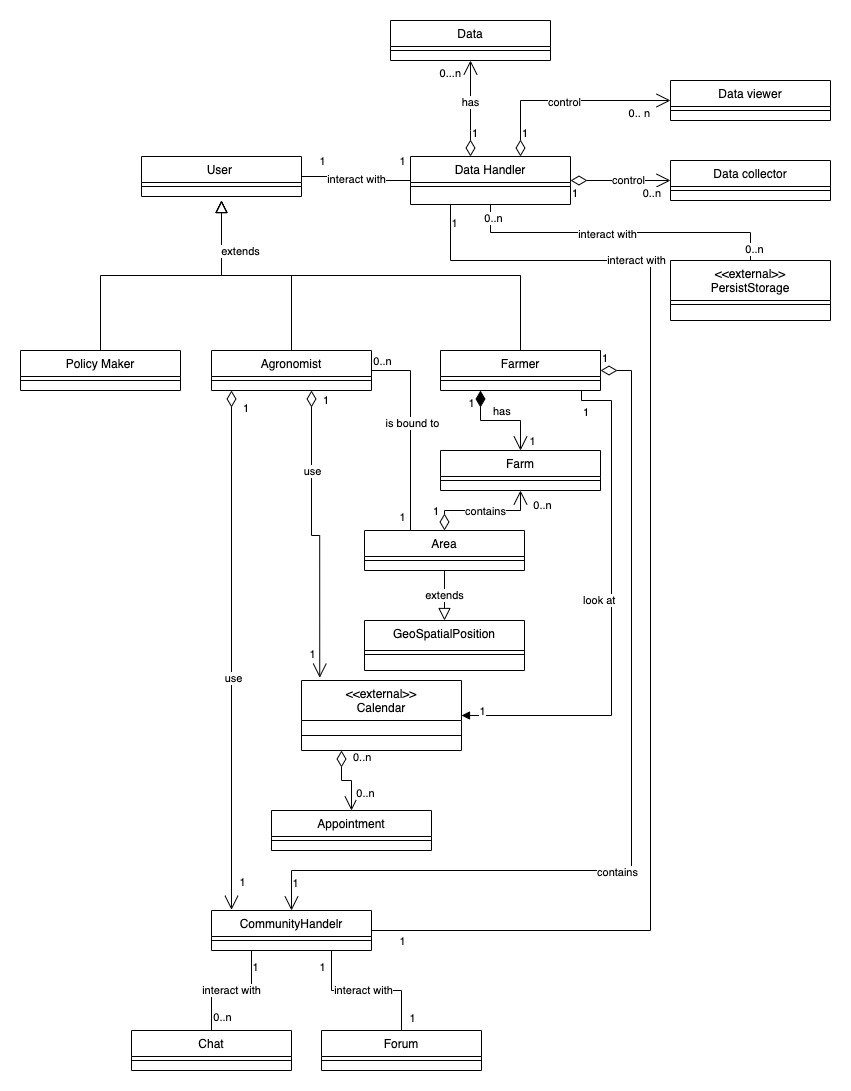
\includegraphics[width=350px]{Class diagram/Class-diagram.jpg}
    \caption{Class Diagram}
\end{figure}

\subsection{Scenario 1 (Use case: 1.1, 2.1, 3.1)}
Adahy is a Farmer that lives in telangana, he has some problems with his farm because of India's climate and the little amount of water available, as do a lot of his colleagues. Adahy heard about a new application that proposes to help Farmers with the decision making process using new informatic technologies and the help of professional agronomists.\\
Adahy picks up his phone, goes on his app store and downloads the DREAM application. He clicks on “Sign up” and the sign up interface shows up, he inserts the email and chooses a password. He confirms his email by clicking on the link on his personal inbox email. The system shows him a list of fields to be filled with Adahy’s role, after he expresses his role as farmer, the system opens a form to insert his Farm information fiel, so Adahy does so. Another confirmation mail is received by Adahy and the sign up is completed.
\subsubsection{Please note}
The dual scenario for the agronomist’s registration has not been written in order to avoid redundancy. It would have been the same as the Farmer’s, the only thing would have changed is the fact that the agronomist does not insert data about the farm, instead, they insert data about which area they make themself available to be assigned to. So, scenario 1 can also map the use case 2.1. Also the Policy Maker's registration use case, the number 3.1, can be mapped into this scenario and, also here, there would be not the insertion of farm's data, but the insertion of the Policy Maker's personal data only.

\subsection{Scenario 2 (Use case: 1.2, 1.3, 1.4, 1.6)}
Ravi is a Farmer that is already registered on the DREAM application. He is facing some problems with his plantation due to the drought, so decide to open a ticket so that he can chat with an Agronomist. Within two hours Yamir, one of the agronomists, accepts the chat request and starts the chat with Ravi. After a few days of chatting, Ravi decides it’s better to ask the agronomist to come to Ravi's farm for a visit and write to Yamir about this. The agronomist advises Ravi to use the proper button to request for a visit while the agronomist sends him a proposal to close the chat that Ravi accepts because the chat is no longer needed.
Ravi moves to the home screen where clicks on the “Request for a Visit” button, he fills up all the fields needed describing his problem and submit the request. 
After a few days Ravi receives a date proposal for the visit he requested and decides to accept it, after accepting it the confirmation frame is shown.  

\subsection{Scenario 3 (Use case: 1.5)}
Hemang is a farmer registered into the DREAM system, he has a scheduled visit for tomorrow. Unfortunately, Hemang is not at home tomorrow because he has to work at one of his colleague's farm, so he goes to the scheduled visit screen and clicks on the “Reject” button related to the visit of tomorrow. By doing so, the agronomist receives a notification about the canceled appointment.

\subsection{Scenario 4 (Use case: 1.7, 1.8, 2.6, 2.7)}
Ganaraj wants to share his thoughts about the new seed he wants to plant, that’s a perfect topic for the DREAM forum. Ganaraj clicks on the forum button, then on “open a thread”, decides the title and the body of the post and then publishes it, receiving within 6 hours lots of comments from some colleagues from other areas. 
Satisfied about the participation on his new thread, Ganaraj decides to look for other interesting topics on the Form and he finds a thread about a machine that he used, so he opens the thread, clicks on “comment” and writes about what was his experience, publishing the comment.  
\subsubsection{Please note}
As also in \textit{Scenario 1}, here we map also scenario 2.6 and 2.7 which are the agronomist's ones, because the scenario would have been very similar to this one.
\subsection{Scenario 5 (Use case: 1.9)}
Dinpal is a farmer registered into the DREAM system, he is happy about the fact he signed up to it, because the agronomist of his area helped him during the production process and now he is proud about the results. In order to keep track of his results, so that he can remember how he achieved this goal of production, Dinpal opens the DREAM application and clicks on “ production data '' button. A list of fields shows up on the interface, Dinple fills them up and clicks on “confirm”. Now the data about Dinpal’s production are stored.

\subsection{Scenario 6 (Use case: 0.2)}
Esh is a farmer already registered in the DREAM application, he is curious to know which crop is planted in land like his. So, he clicks on “visualize data”, the system shows a dashboard with data about Esh’s farm, like the soil composition, meteo forecasts and agronomist suggestions and so on. Esh sees that there is also the possibility to filter and fetch other types of data and decides to look for types of crop that have been planted in soil like his. The system shows him an interface where data are visualized.
\subsection{Scenario 7 (Use case: 2.2, 2.3, 2.4)}
Yamir is an agronomist already registered in DREAM. He receives a notification about a new ticket opened into the system, so he opens the “chat interface” where there are the pending chats that are visible to all the agronomists of the same area. He decides to take charge of the new chat request, so he clicks on it, and then “process request”. After some days of chatting with Ravi, who is the Farmer who opened the ticket, it is proposed to Yamir to go to visit Ravi’s farm to solve the problem, so Yamir invite Ravi to go on his interface and look for the proper button to request for a visit and in the meanwhile Yamir sends a proposal to close the chat. Ravi does as Yamir said, he closes the chat. Yamir goes on the screen where the farms assigned to his area are listed. Yamir notices that Ravi’s farm went up in rank, due to the chat request which has just been done, he clicks on it and chooses a date to propose and send the proposal. 
After a while Yamir receives the confirmation to visit Ravi’s farm on the date Yamir proposed.

\subsection{Scenario 8 (Use case: 2.5)}
Chandra is an agronomist registered in DREAM. It's noon when he finishes visiting Dharesh’s farm. He is happy about the visit because Dharesh was having doubts about when to harvest but now they are solved. Chandra opens DREAM, goes in the schedule screen, where there is the list of the scheduled visits of the day, and clicks on "Done" where Dharesh's farm is written. Now compile the report of the visit, skipping the measures screen, and clicks on "Confirm". Now the report is sent and it's all done. \\ 
On tomorrow Chandra has Gopan's farm in schedule, but he thinks that's not more necessary because Gopan called him on the phone and they already solved Gopan's problem. So, Chandra goes on tomorrow's schedule and clicks on "Cancel", by doing so the appointment for tomorrow has been deleted and a notification has been sent to Gopan.
\subsection{Scenario 9 (Use case: 3.2)}
Harish, a Policy Maker registered in DREAM, wants to control the effect of DREAM on Telangana, he opens the application and goes to the performance screen, the system shows him a rank of farms ordered by performance score. Harish is very happy about this system because it simplifies his work a lot and allows him to see all the history of each farm. Therefore, now Harish can analyze the history of the data of the first farm of the rank in order to understand which kind of steering initiatives the government can propose.
\section{Product Functions}
\subsection{Sign Up and Login}
These functions will be available to all the users.\\ \\
The sign up functionality allows users to register themselves to the website. In particular, each user will be asked to provide an email (the email will be the username of the user) and a password. If the email is not registered yet (a user can not register themselves twice) a verification email is sent to the user. Once the user has confirmed the email, the system will ask them which actor of the system they represent (farmer agronomist or policy maker), and depending on this choice the system will ask the user to insert role specific data, for example:\\
\begin{itemize}
    \item A farmer will be asked to insert data regarding their farm
    \item An agronomist will be asked to insert the area in which she/he works and their professional code (this code will be used by the system's administrators in order to control if the agronomist is a real agronomist)
    \item A policy maker will be asked to identify themselves
\end{itemize}
The login functionality will allow registered users to login in the system by using the correct email and password tuple provided during the registration phase.
\begin{figure}[H]
    \centering
    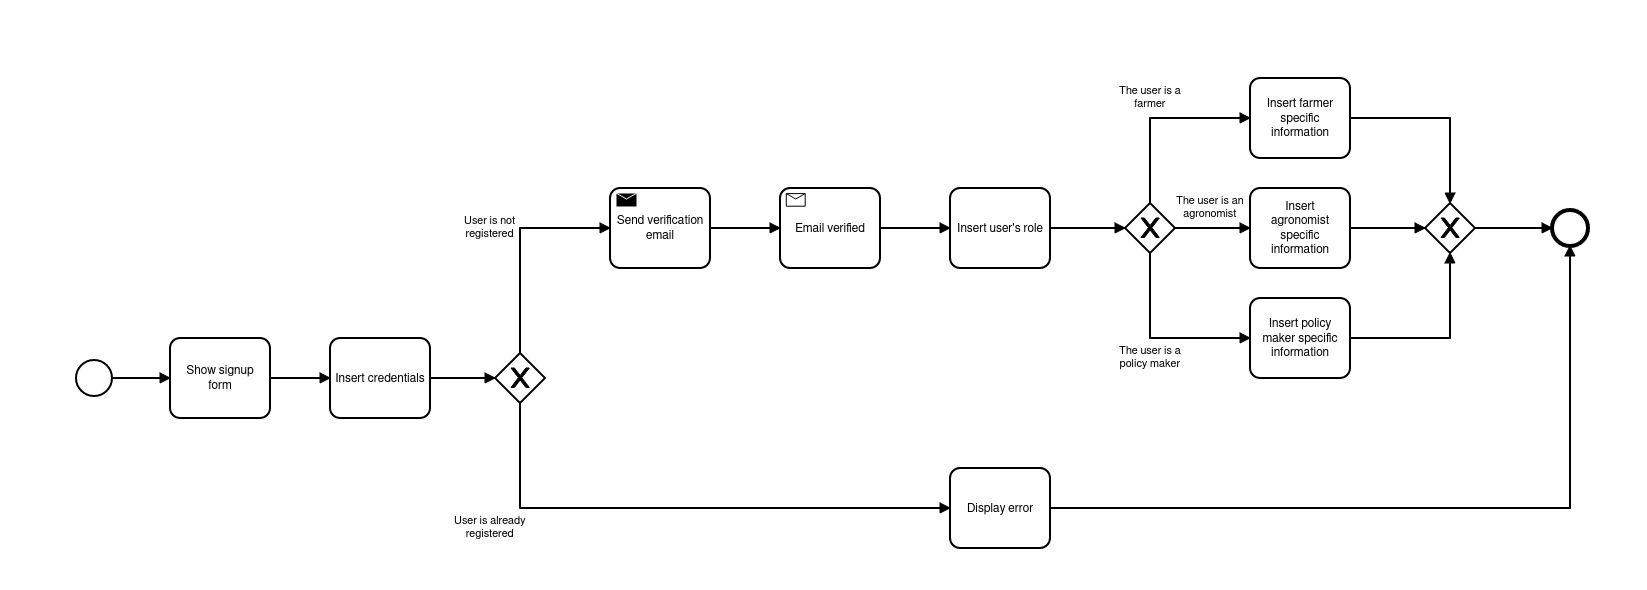
\includegraphics[width=350px]{BPMN/BPMN 221a.png}
    \caption{BPMN for the "Sign Up" functionality}
\end{figure}
\begin{figure}[H]
    \centering
    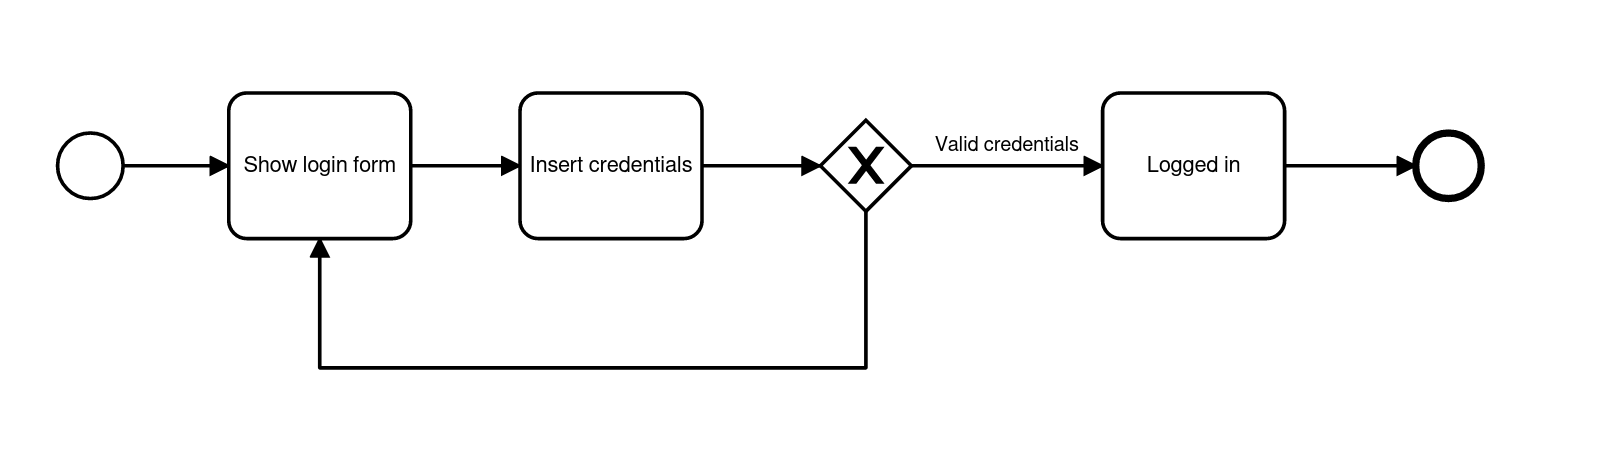
\includegraphics[width=350px]{BPMN/BPMN 221b.jpg}
    \caption{BPMN for the "Login" functionality}
\end{figure}
\subsection{Consult data}
This function will be available to all users.\\ \\
Each user will be able to query the system in order to retrieve data. In particular, each user will be able to access different type of data:
\begin{itemize}
    \item Each farmer will be able to see data regarding their farm and personalized suggestions on how to be more productive and weather resilient.
    \item Each agronomist will be able to see data regarding each farm in their area and data regarding the area they are responsible for as a whole. Moreover each agronomist will be able to see which farmers belongs to their area.
    \item Each policy maker will be able to see data about all the farms in Telangana and about each area in which Telangana is split in.
\end{itemize}
\begin{figure}[H]
    \centering
    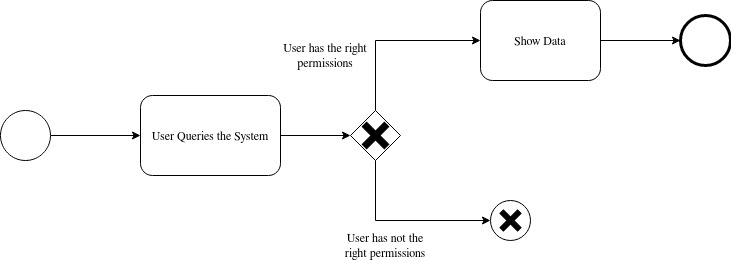
\includegraphics[width=350px]{BPMN/BPMN 222.jpg}
    \caption{BPMN for the "Consult data" functionality}
\end{figure}
\subsection{Insert data}
This function will be available to agronomists and farmers.\\ \\
This functionality will allow agronomists and farmers to insert data into the system. In particular, the system will allow farmers to insert data about the production of the farm, while the agronomist will be able to insert data regarding measurements taken during their visits. Moreover, agronomists will be able to insert a report of each farm they have visited.
After the insertion of data the system must validate them, making sure that the inserted data makes sense.
\begin{figure}[H]
    \centering
    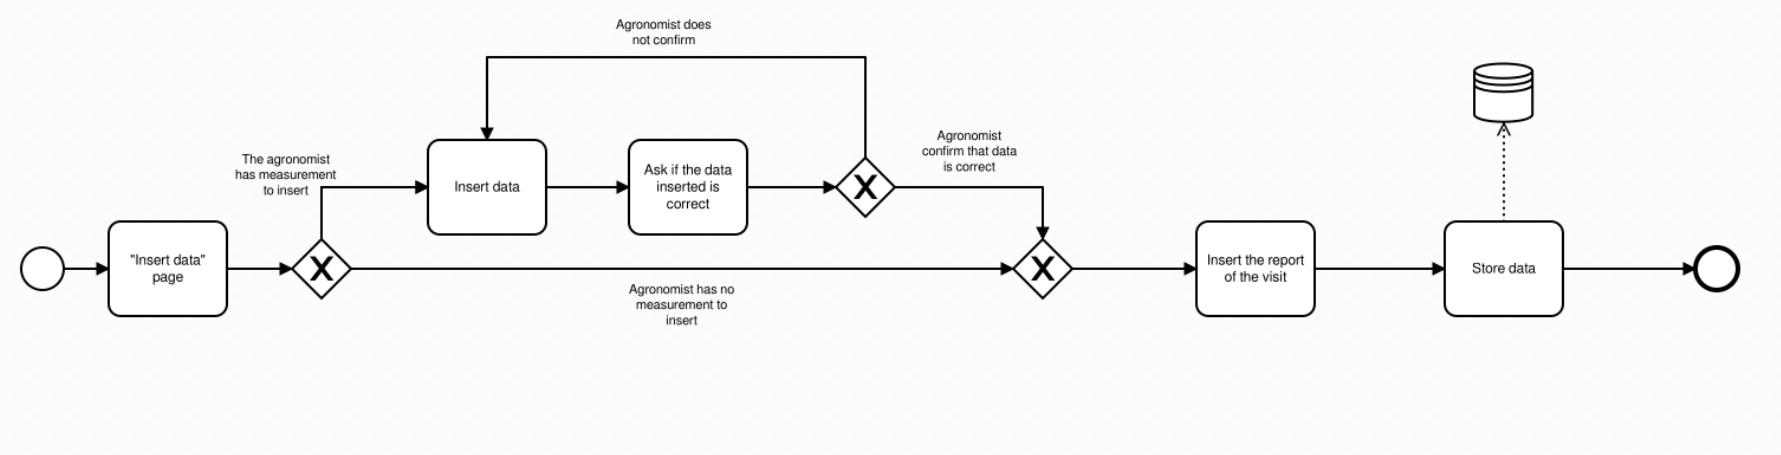
\includegraphics[width=350px]{BPMN/BPMN 223a.jpg}
    \caption{BPMN for the "Insert data" functionality, agronomist's side}
\end{figure}
\begin{figure}[H]
    \centering
    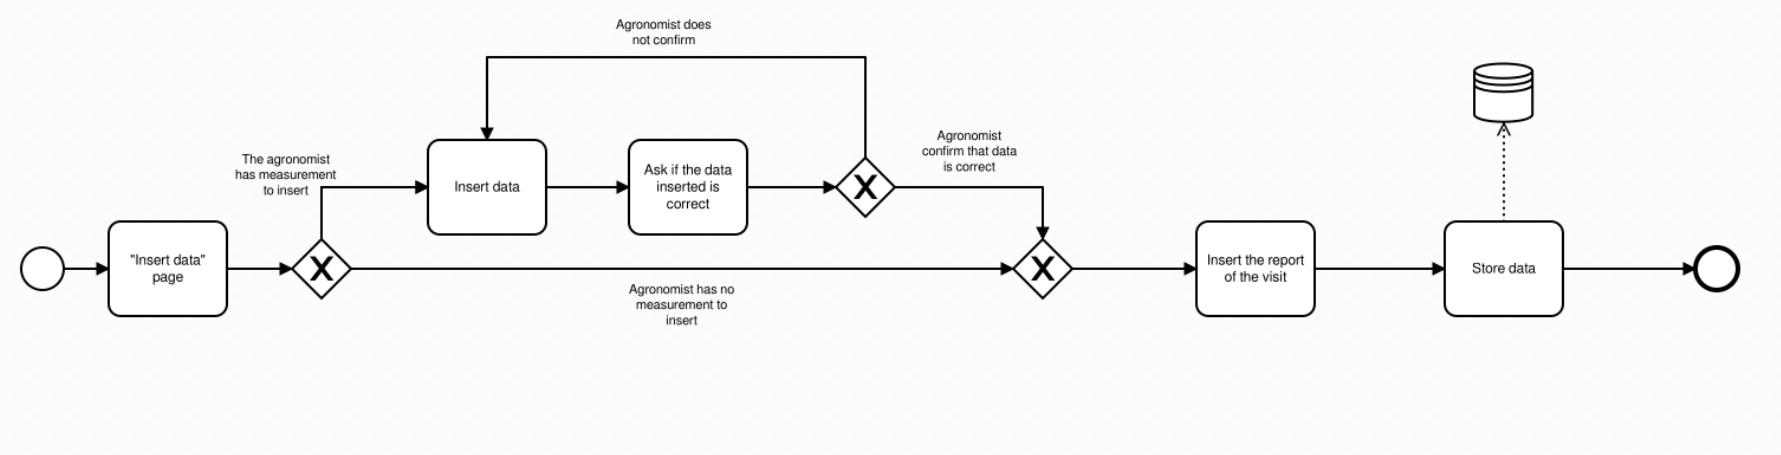
\includegraphics[width=350px]{BPMN/BPMN 223a.jpg}
    \caption{BPMN for the "Insert data" functionality, farmer's side}
\end{figure}
\subsection{Chat between farmers and agronomists}
This function will be available to farmers only.\\ \\
The system will allow farmers to request the help of an agronomist by using a chat. In particular a farmer can open a ticket asking for the help of an agronomist responsible for their area. An agronomist then can handle the ticket, thus opening a chat. The system therefore will allow the two to communicate through the chat. Once the problem is solved, the agronomist will be able to close the chat.
\begin{figure}[H]
    \centering
    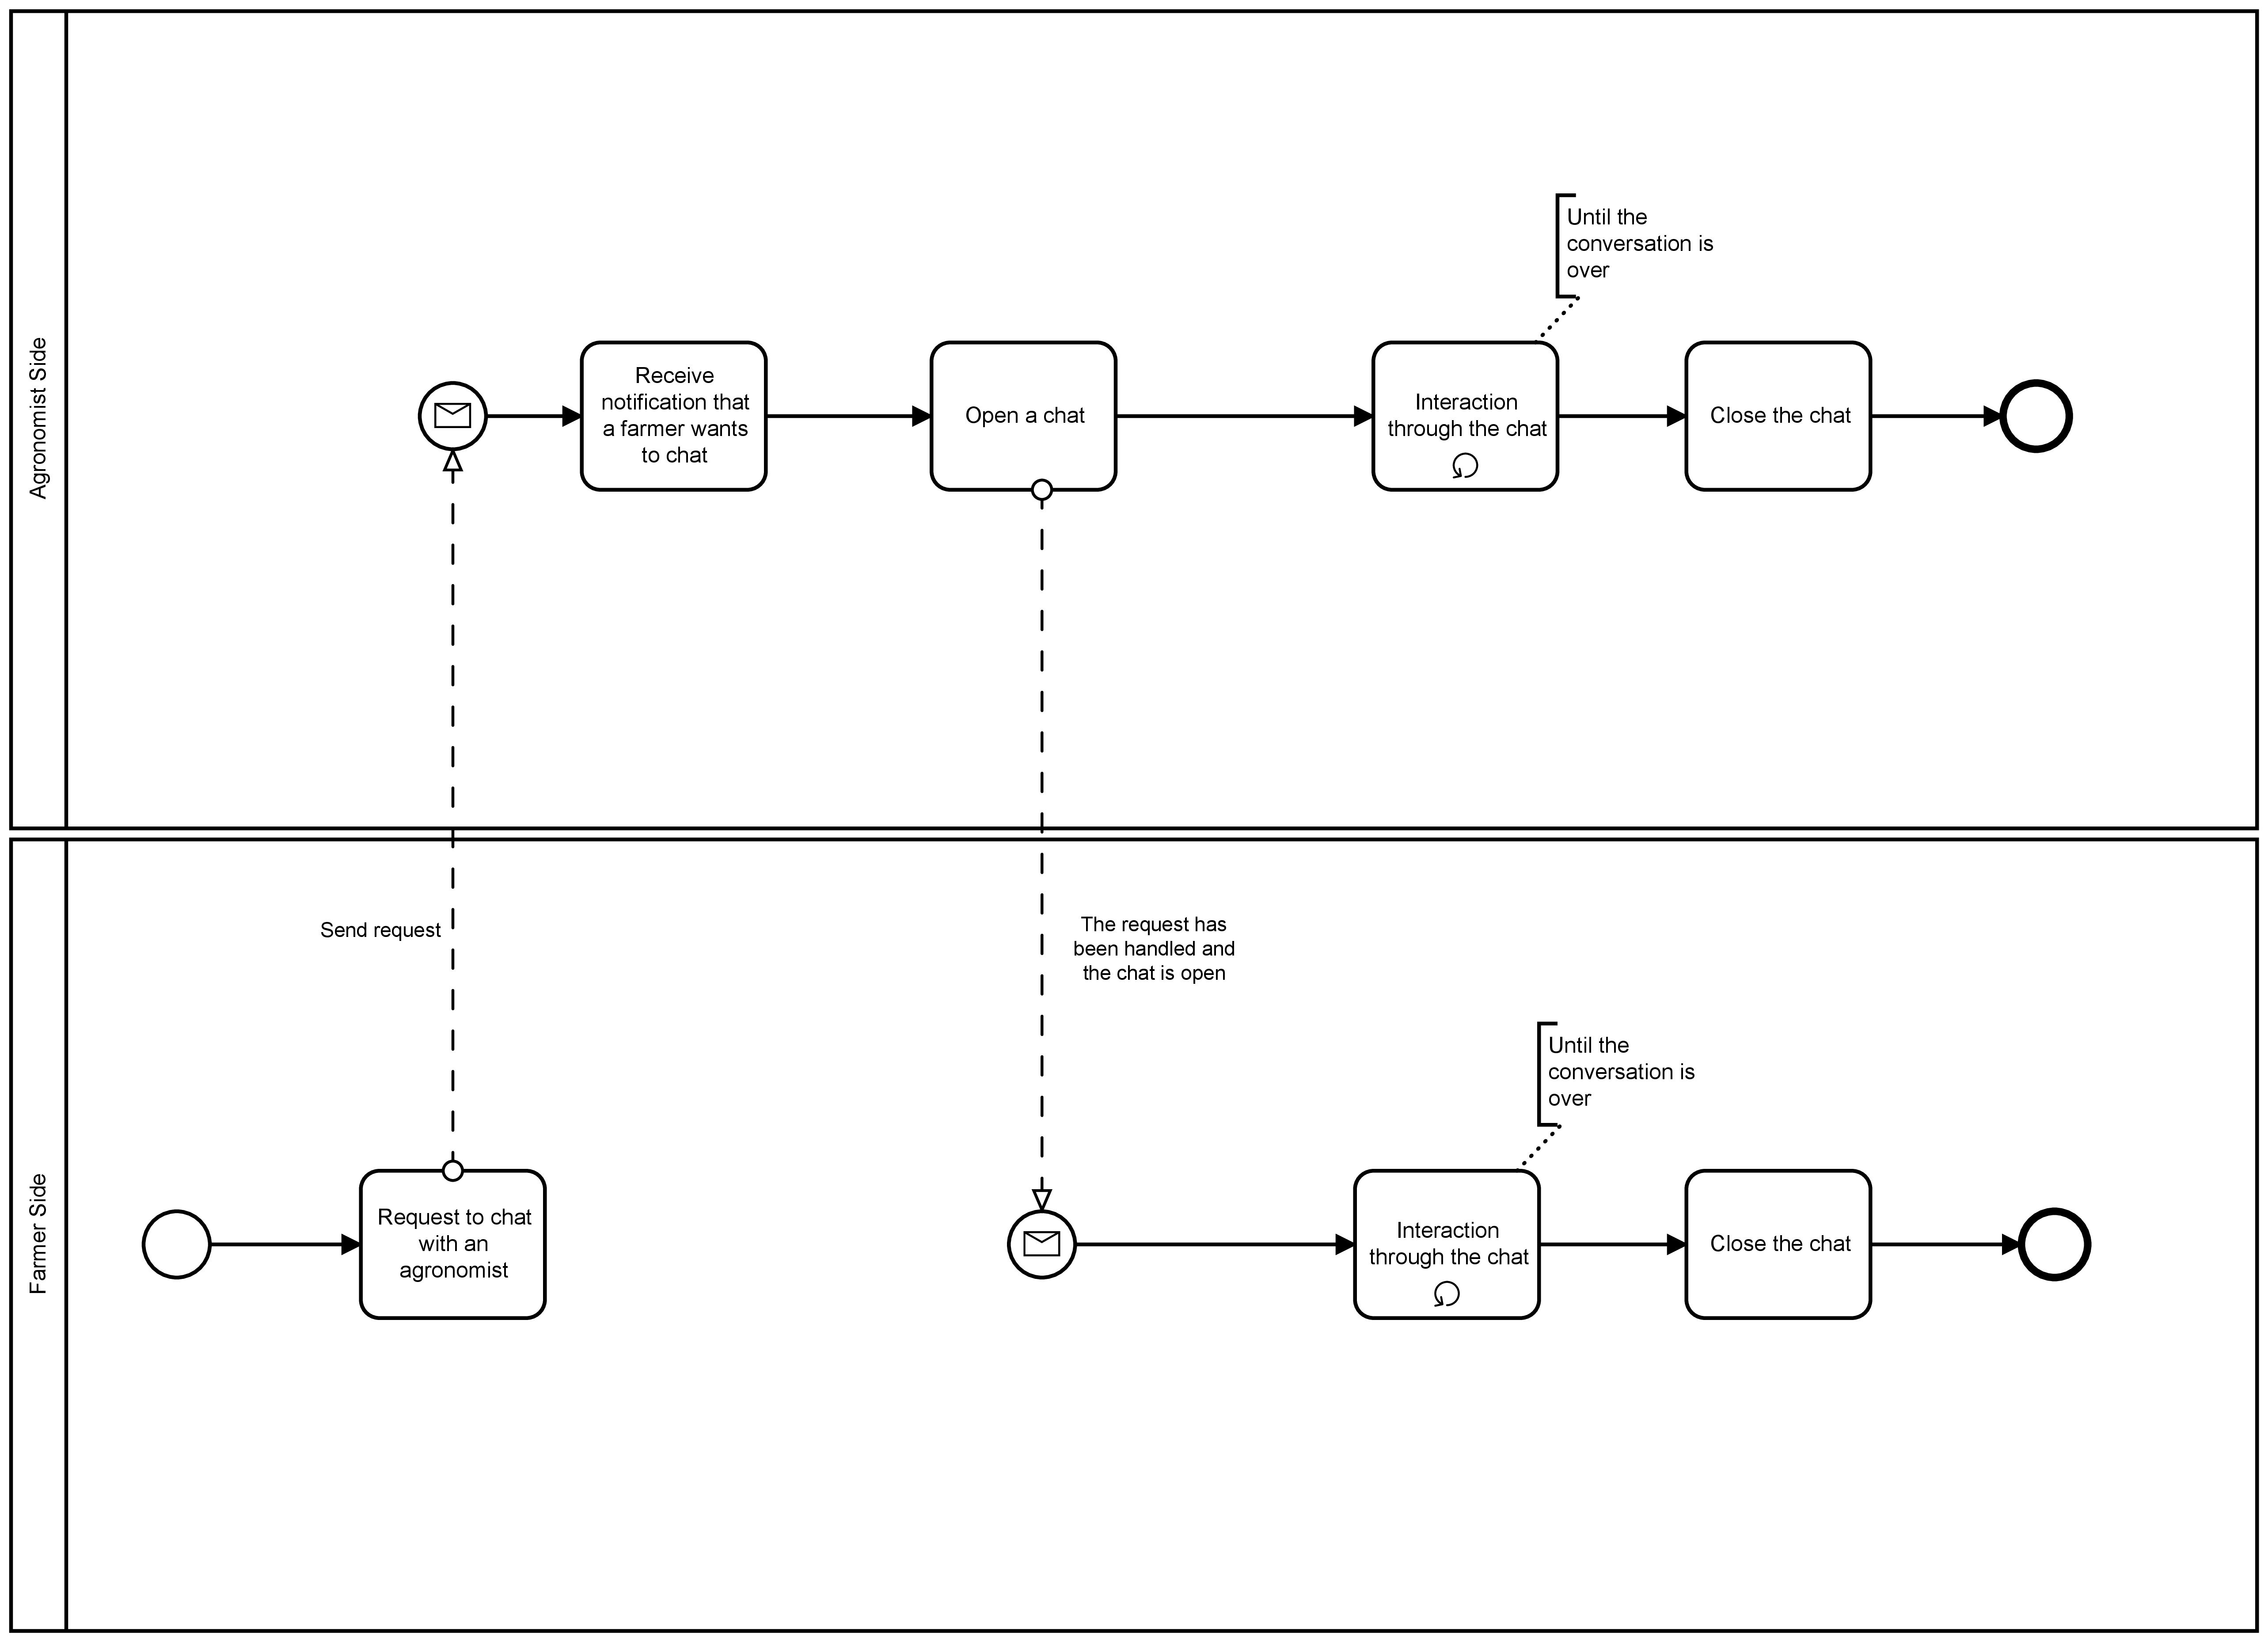
\includegraphics[width=350px]{BPMN/BPMN 224.jpg}
    \caption{BPMN for the "Chat between farmers and agronomists" functionality}
\end{figure}
\subsection{Request a visit by an agronomist}
This function will be available to farmers.\\ \\
The system will allow farmers to request an agronomist to visit their farm in order to help them. In particular, the farmer will be able to request a visit through the system. Once the request has been sent, it will be received by all the agronomists responsible for the area the farmer belongs to, and it can be handled by one and only one among the agronomists. In order to handle the request, an agronomist will schedule a visit in their schedule. This will cause the system to send a notification to the farmer informing them that a visit has been booked, showing them both the date and the time of the visit.
\begin{figure}[H]
    \centering
    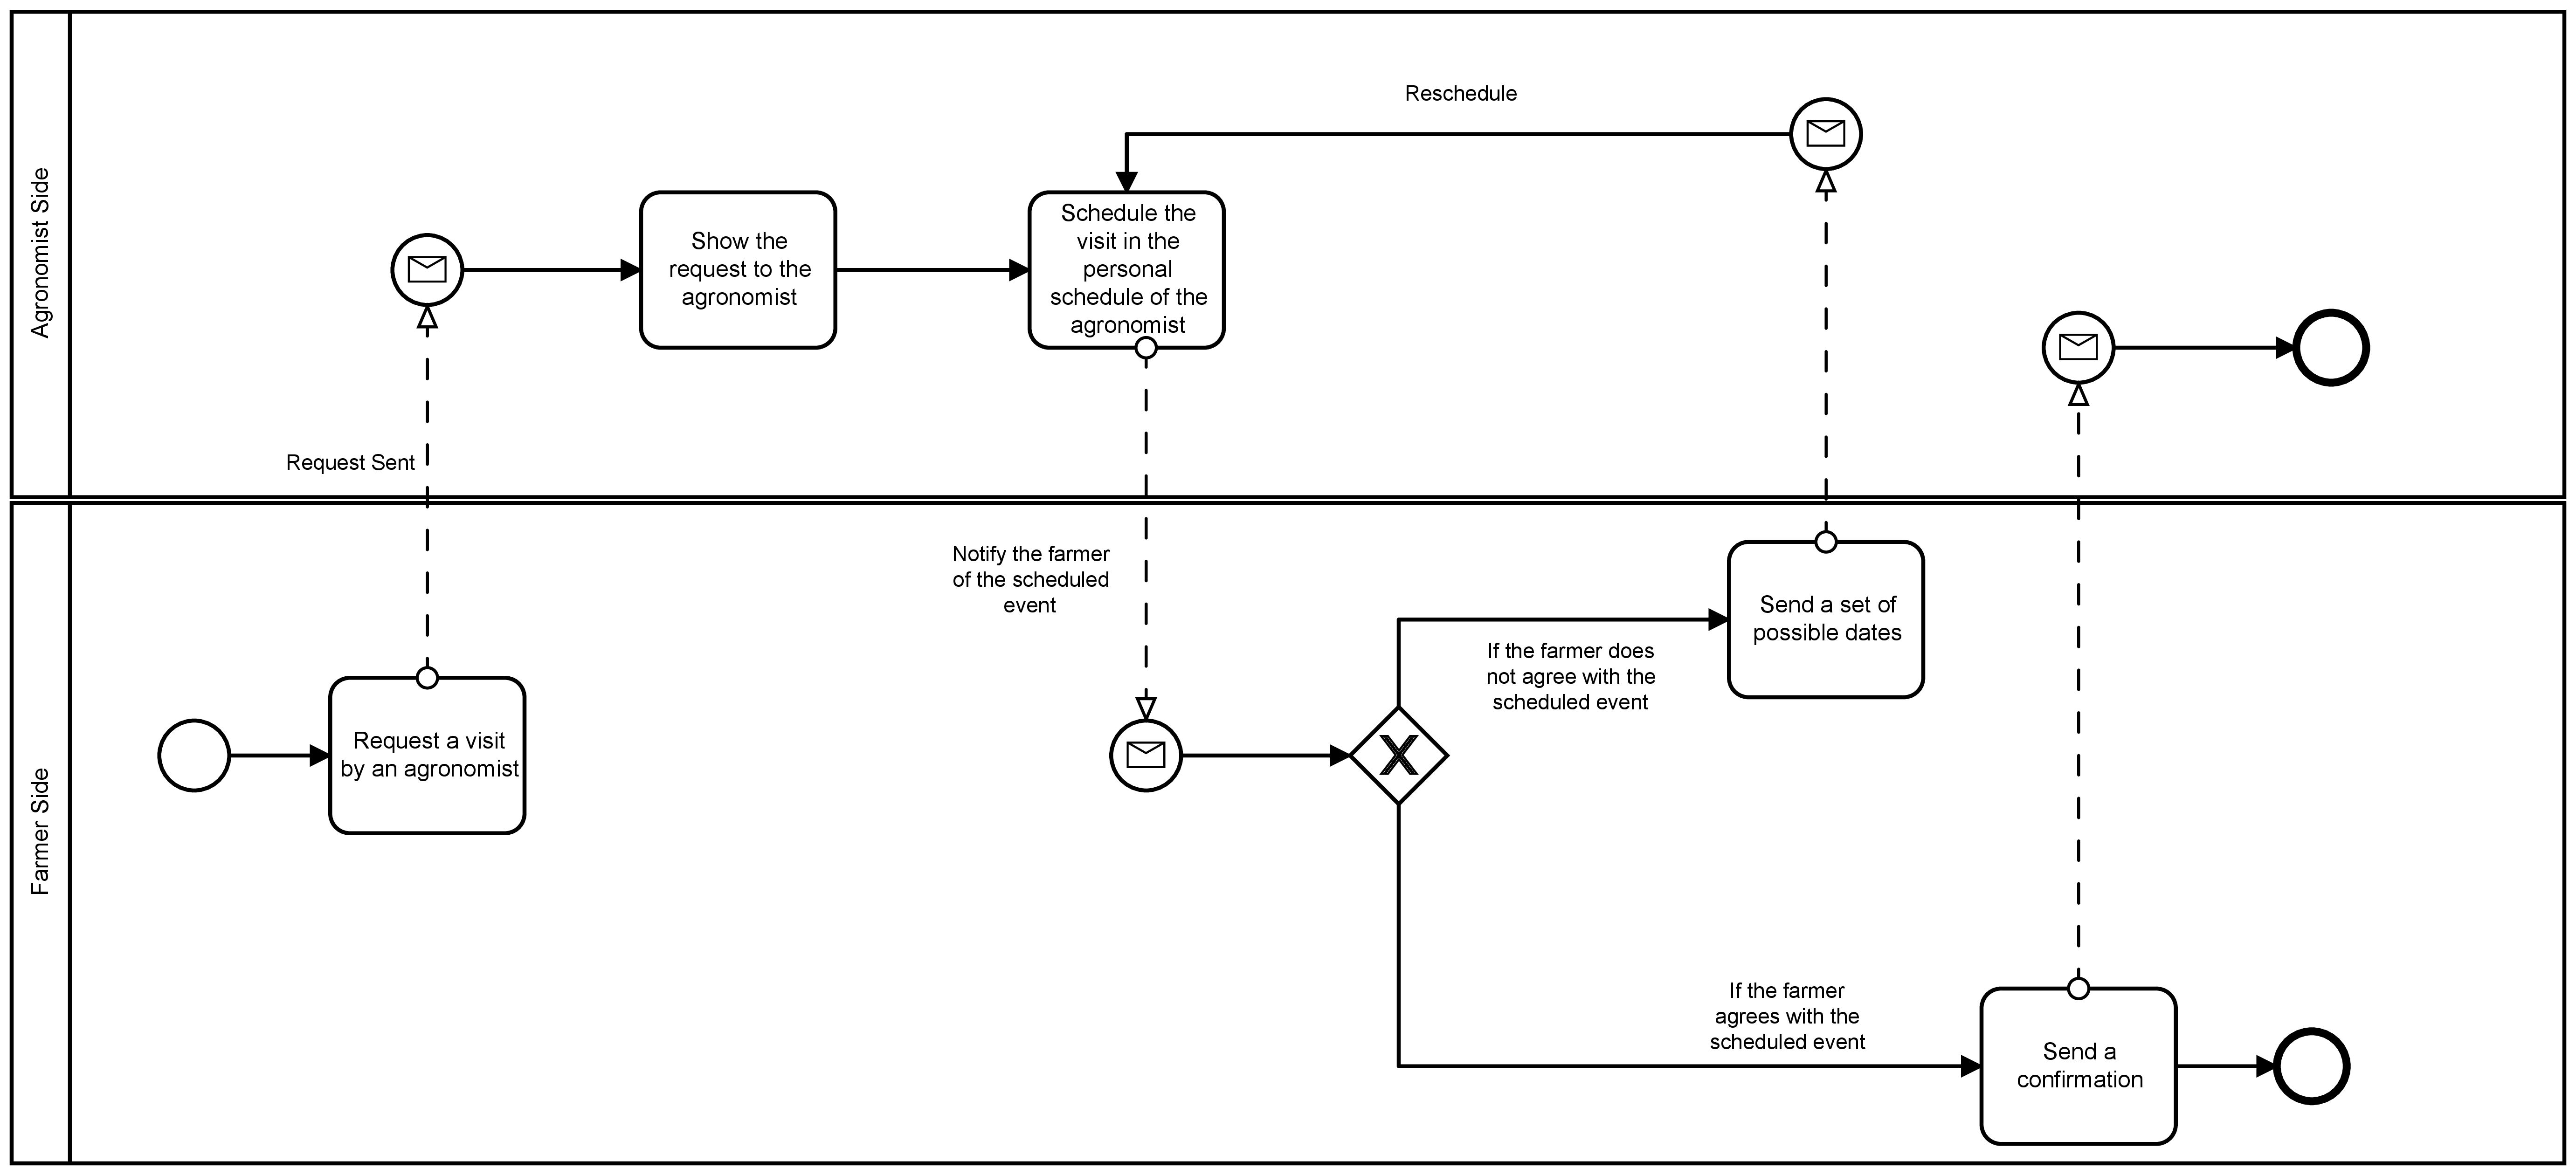
\includegraphics[width=350px]{BPMN/BPMN 225.jpg}
    \caption{BPMN for the "Request a visit by an agronomist" functionality}
\end{figure}
\subsection{Interaction between farmers and agronomists through a forum}
This function will be available to farmers and agronomists.\\ \\
The system will allow farmers and agronomists to interact through a forum. In particular, each of them will be able to open a new thread or to write into an existing one.
\subsection{Schedule a visit to a farm}
This function will be available to agronomists.\\ \\
Because all farms must be visited at least twice a year, and those that are under-performing should be visited more often, this functionality will allow an agronomist to see the list of farms they are responsible of, ordered by priority (first the ones who are performing poorly and the ones who requested for a visit). By consulting this list the agronomist will be able to schedule, in their schedule, one or more visits to the various farms who need help. By scheduling a visit the priority of the farm will decrease and a notification will be sent to each scheduled farmer.
\begin{figure}[H]
    \centering
    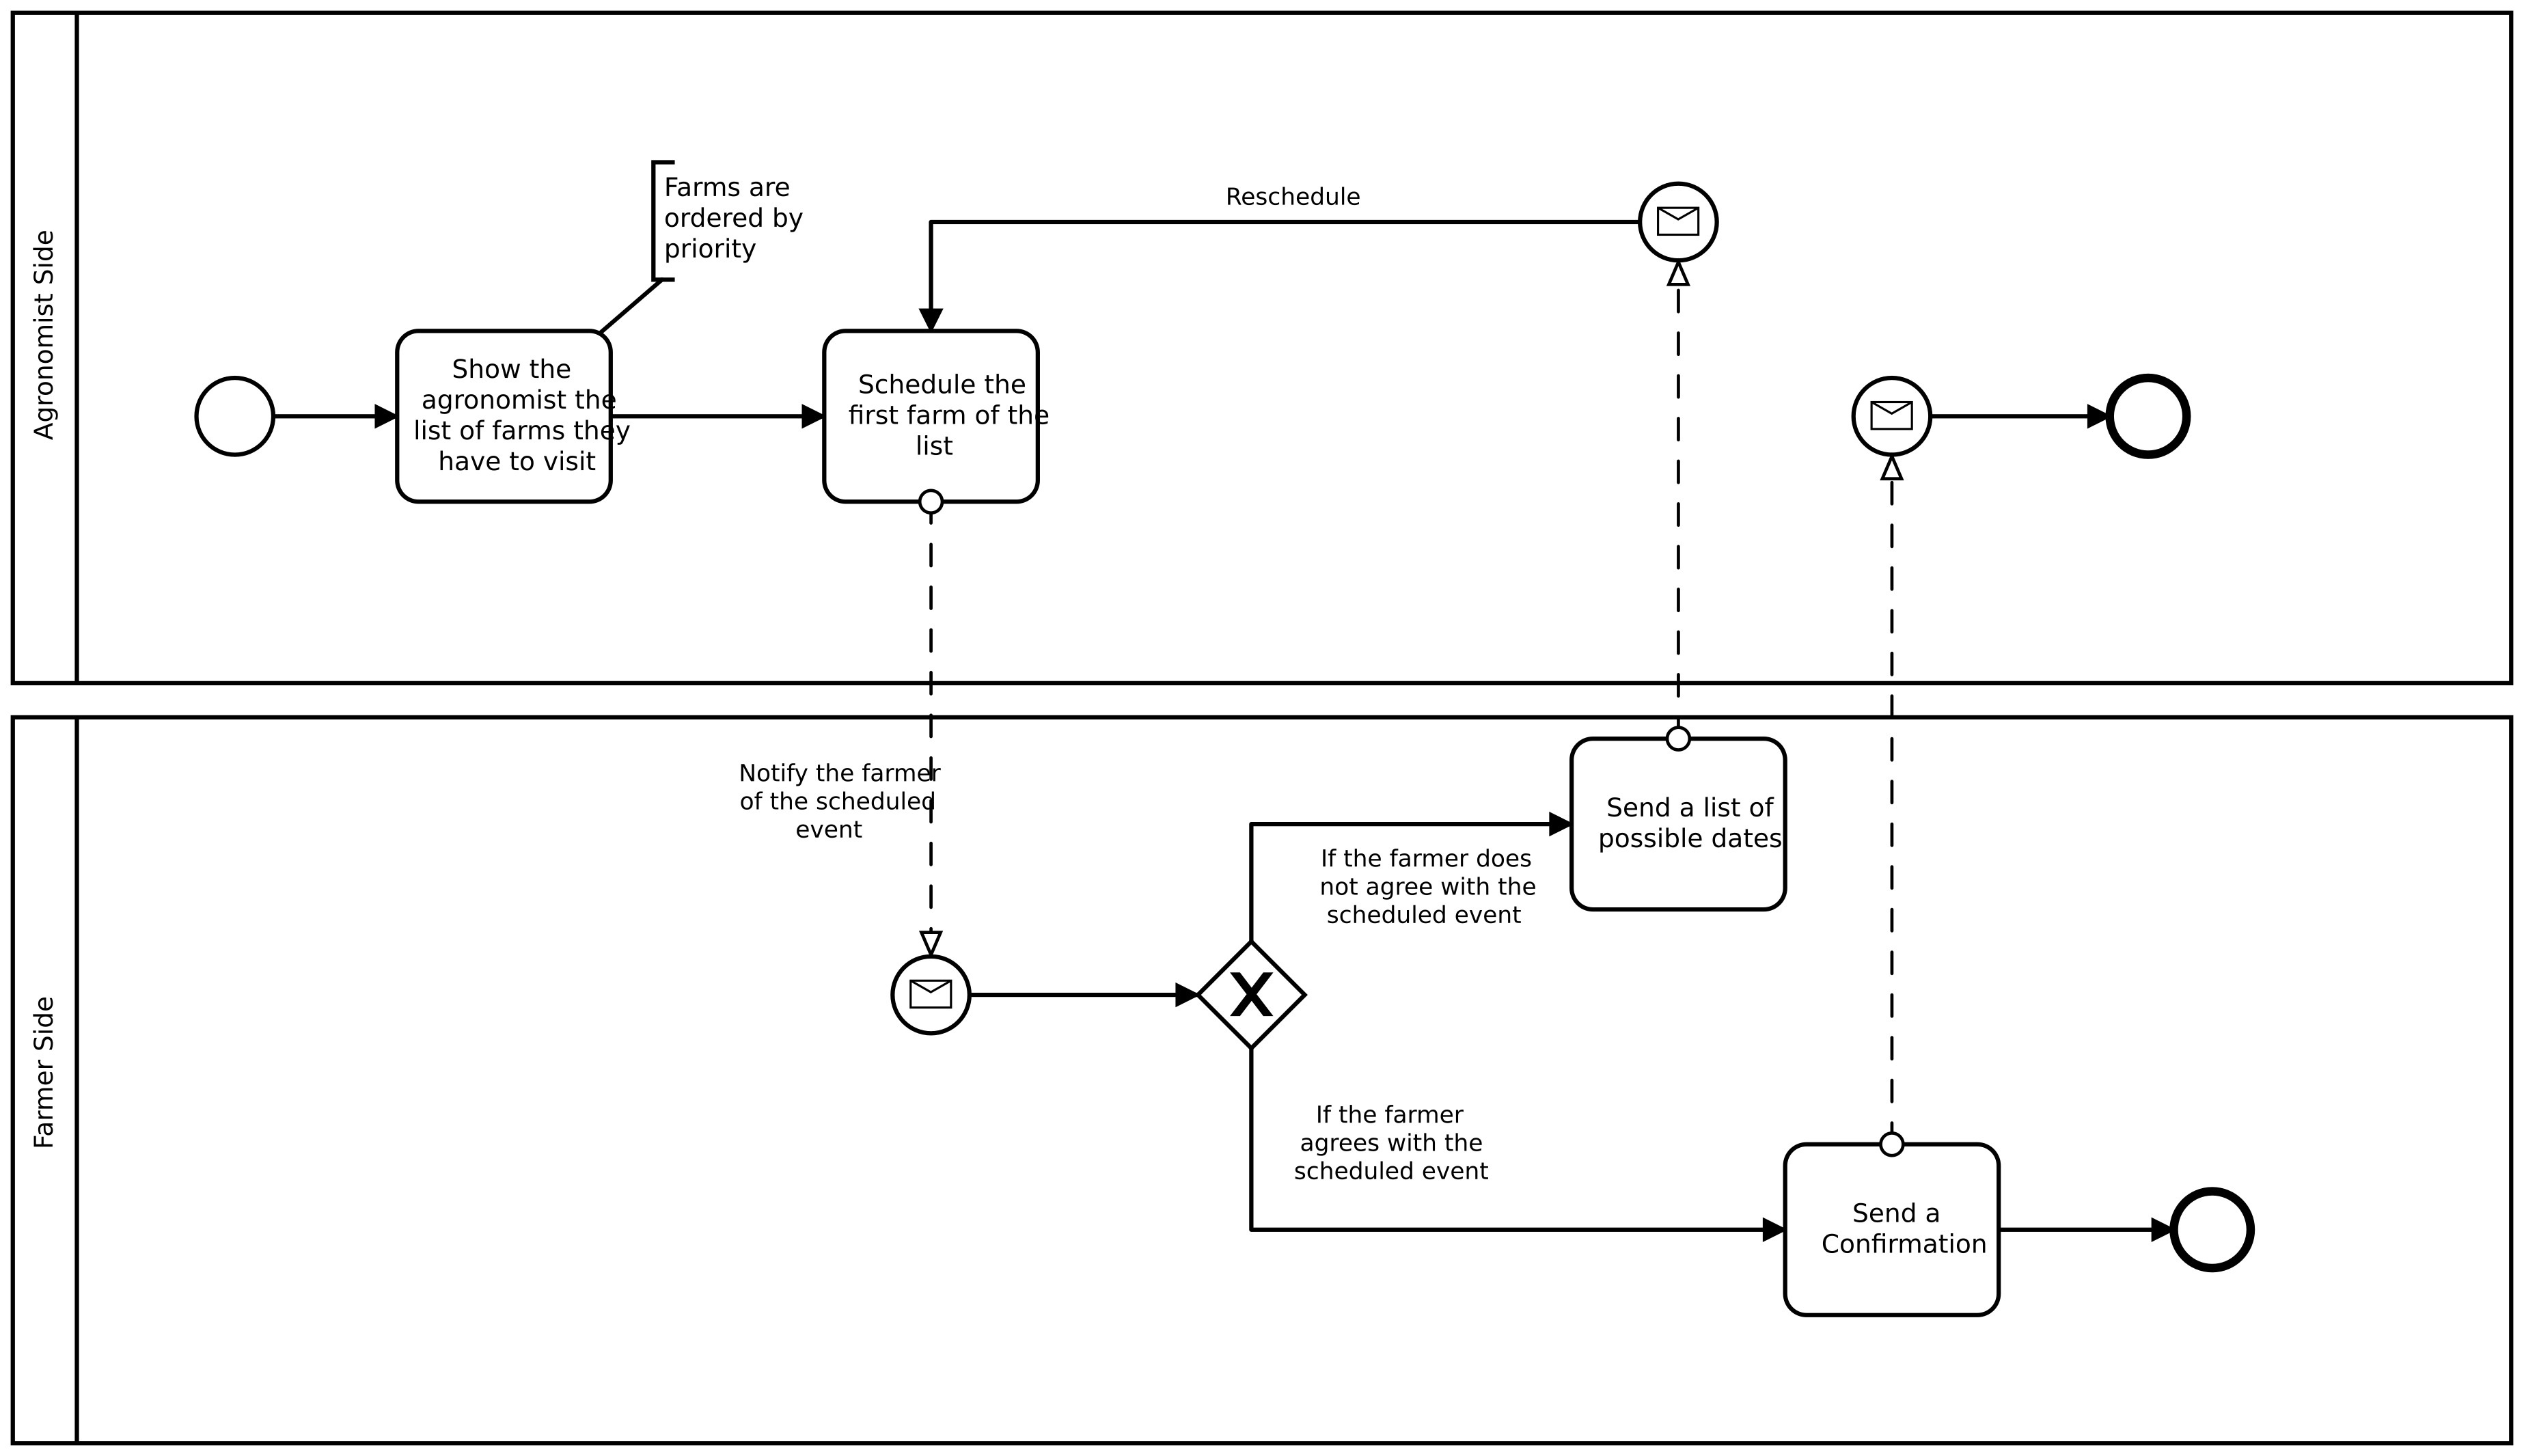
\includegraphics[width=350px]{BPMN/BPMN 227.jpg}
    \caption{BPMN for the "Schedule a visit to a farm" functionality}
\end{figure}
\subsection{Confirm the daily schedule}
This function will be available to agronomists.\\ \\
At the end of each day each agronomist will be able to confirm the visits done during the day. In particular, each agronomist will be able to insert data measurements taken during the daily visits, and they will be forced to write a report for each farm they have visited. If an agronomist did not visit a scheduled farm, for whatever reason, no report will be inserted and the system will increase the priority of the farm in order to make it appear on top of the list of all the farms of the area.
\begin{figure}[H]
    \centering
    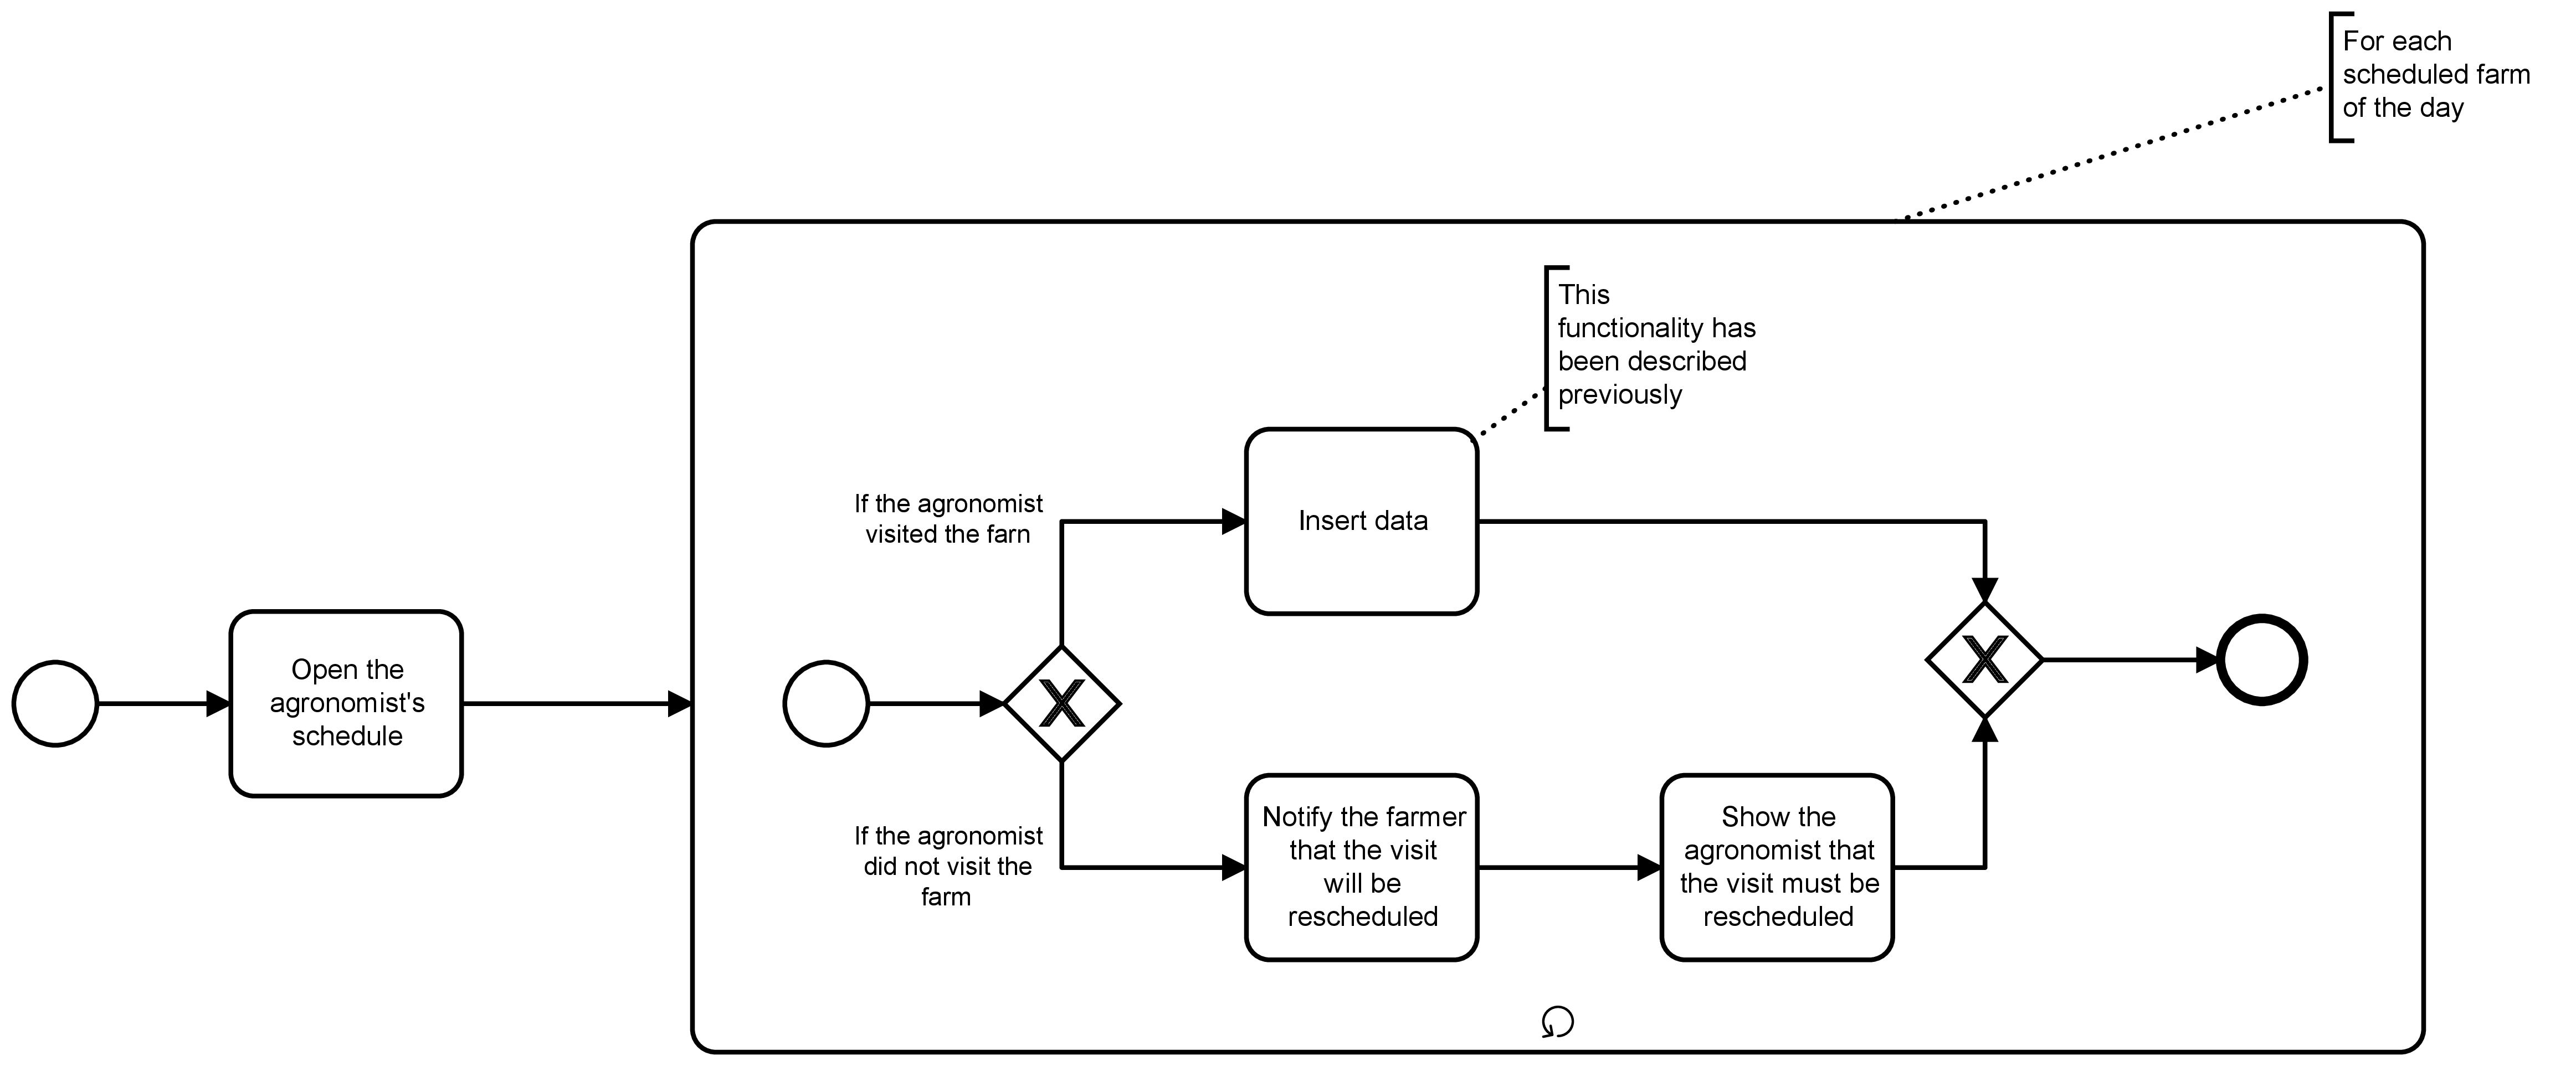
\includegraphics[width=350px]{BPMN/BPMN 228.jpg}
    \caption{BPMN for the "Confirm the daily schedule" functionality}
\end{figure}
\subsection{Cancel a scheduled visit}
This function will be available to agronomists.\\ \\
In every moment an agronomist will be able to cancel a scheduled event in their schedule. The system then will notify the farmer that the scheduled event has been canceled. Moreover, the system will increment the priority of the farm in order to make the agronomist keep in mind that the visit must be rescheduled as soon as possible.
\begin{figure}[H]
    \centering
    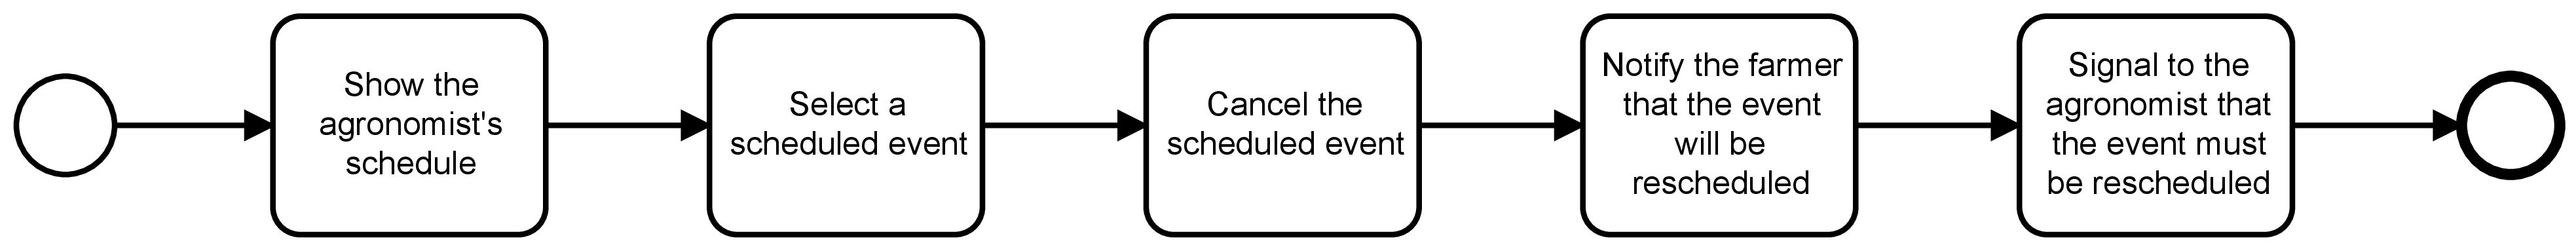
\includegraphics[width=350px]{BPMN/BPMN 229.jpg}
    \caption{BPMN for the "Cancel a scheduled visit" functionality}
\end{figure}
\subsection{Fetch data}
The system will periodically fetch data from different available databases. Once fetched, data will be cleaned, transformed in order to make them homogeneous, and analyzed in order to extract new knowledge from them. In particular, the system will be able to infer which farms are performing particularly well and the ones which are performing poorly (e.g. by leveraging machine learning and in particular clustering).
\begin{figure}[H]
    \centering
    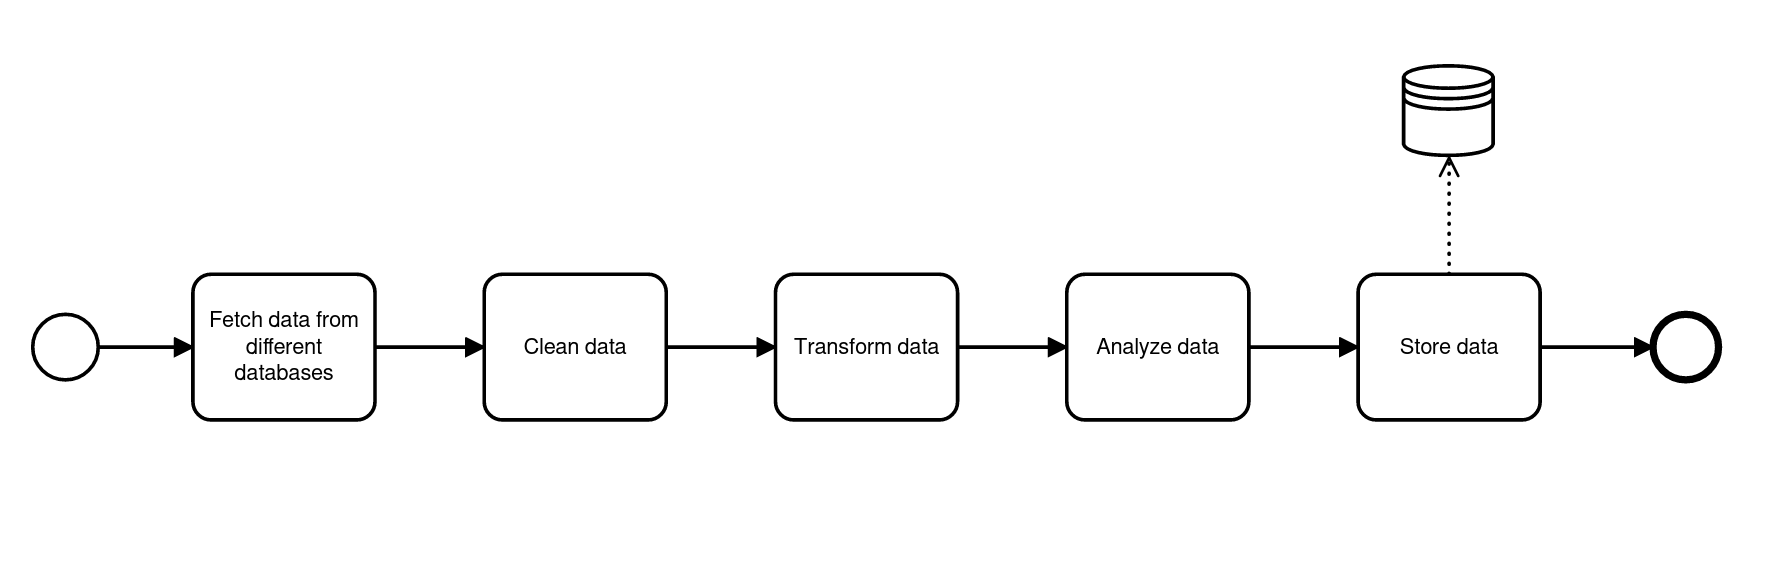
\includegraphics[width=350px]{BPMN/BPMN 2210.png}
    \caption{BPMN for the "Fetch data" functionality}
\end{figure}
\section{User Characteristics}
\subsection{Policy Makers}
They are the government users, they are interested in knowing how Telangana’s Farmers are performing and they want to know why and how the performances are going so. Using their dashboard they will be able to see, filter and compare all the data stored in the system matching also with the report written by the agronomist. Studying the most effective strategies against meteorological adverse events in order to help spread out the best practice.

\subsection{Farmers}
A farmer is a person who has one or more pieces of land and wants an external, possibly professional, support in order to choose the better strategy to maximize the harvest, deals with problems that can derive from the climate and also which product is better to use considering the land he is cultivating. They will be in contact with other farmers through a forum so that they can exchange advice on the cultures. 
They will be able to contact both agronomists using the forum and/or one of the Agronomists who are assigned to the same area the Farmer is assigned as well, in order to get any help. 
\subsection{Agronomists}
An Agronomist is a professional figure that decides to sign up into the DREAM project as a user who will take into account an area to which more farmers are associated.
Being a professional figure, the Agronomist will be able to solve Farmer’s problems by giving them advice such as which fertilizer they should use, when they should do the harvest and so on. 
They will use the application to see how Farmers all over Telangana are performing, in terms of culture performance and will do visits to the farms that need it. Every Agronomist will be asked to produce a report so that the strategies applied to each farm are tracked. 
They can use a dashboard in order to filter the available data so that they will be able to compare different farms and so. 

\section{Domain Assumptions}
    \begin{enumerate}[label=(D\arabic*), font=\itshape]
        \item There are enough agronomists for each area
        \item Every user has an internet connection in order to interact with the system
        \item Every farmer has the capability to interact with the system
        \item Every agronomist has the capability to interact with the system
        \item Every policy maker has the capability to interact with the system
        \item Every farmer has an electronic device in order to interact with the system
        \item Every agronomist has an electronic device in order to interact with the system
        \item Every policy maker has an electronic device in order to interact with the system
        \item The farmers insert true and correct data about their production
        \item The agronomists insert true and correct data about measurements
        \item The reports inserted by agronomists are sufficiently detailed
        \item The agronomists always confirms all the visits that they have done, sooner or later
        \item A visit in an agronomist schedule is confirmed only if it is actually done by the agronomist
        \item All the agronomists have at least decent capabilities of managing and organizing their own schedule
        \item All those agronomist that take measurements do so in a consistent way
        \item The farmers follows agronomist’s advice
        \item Only real and capable agronomists are allowed to subscribe to the system 
        \item Only real and capable policy maker are allowed to subscribe to the system 
        \item The agronomist that wants to visit a farm will reach an agreement with the owner farmer on the day and date of the appointment within about 14 days from the first appointment request
        \item Each farmer’s account owns one and only one farm
        \item Each farm is owned by one and only one farmer
        \item Every user has its own credentials
        \item The credentials used to access the system are not shareable
        \item External databases are correctly and periodically updated
    \end{enumerate}

\chapter{Specific Requirements}
\section{Requirements}
    \begin{enumerate} [label=(R\arabic*), font=\itshape]
        \subsection*{Login}
        \item The system allows users to sign up
        \item Every user can access the system only if they are registered
        \item The system must allow to access the system only if the credentials used are correct
        \item The system must not allow to register two different users with the same username
        \item The system must not allow the same user to register themselves more than once
        \subsection*{Preliminary requirements}
        \item The system shall associate to each area one or more agronomists
        \item The system shall associate each farmer to one and only one area
        \item Each agronomist is associated to one and only one area
        \subsection*{Show data}
        \item The system allows the agronomist to see only the list of farms for which they are responsible of
        \item The system allows the farmer to see data about their farm
        \item The system must not allow the farmer to see data about farms other than theirs
        \item The system allows the agronomist to see data about a specific farm
        \item The system allows the agronomist to see data about the area for which they are responsible for
        \item The system must not allow the agronomist to see data about farms for which they are not responsible for 
        \item The system must not allow the agronomist to see data about an area for which they are not responsible for
        \item The system allows the policy maker to see data about a specific farm
        \item The system allows the policy maker to see data about an area
        \item The system allows the policy maker to see data about all the areas in Telangana
        \item The system must fetch data from different sources containing relevant information for the scope of the application
        \item The system must elaborate and aggregate data fetched from different sources
        \subsection*{Chat between farmer and agronomist}
        \item The system allows farmers to request to have a chat with an agronomist
        \item The system allows agronomists to accept chat requests
        \item The system allows farmers and agronomists to interact through a chat
        \item A farmer, belonging to an area, can chat only with an agronomist belonging to the same area
        \item Each farmer can have at most one open chat at any given time
        \item Each agronomist can have multiple chats open at any given time
        \item The system allows only agronomists to close chats
        \subsection*{Booking a visit}
        \item The system allows farmers to request a visit from an agronomist
        \item The system must show an agronomist a list of farms they have to visit, ordering them by priority
        \item The system must prioritize the farms that need help
        \item The agronomist must prioritize the farms that the system prioritize
        \item The system allows agronomists to schedule a visit at any farm of their competence
        \item The system allows agronomist to set up a daily schedule
        \item The system must notify a farmer when an agronomist schedules a visit to their farm
        \item The system must notify an agronomist when a farmers cancels a scheduled visit to their farm
        \item The system must notify a farmer when an agronomist cancels a scheduled visit to their farm
        \item The system allows agronomists to cancel a scheduled visits within one day before
        \subsection*{Forum between farmers and agronomists}
        \item The system shall allow farmers to interact through a forum with other farmers and agronomists
        \item The system shall allow agronomists to interact through a forum with other agronomists and farmers
        \item The forum allow to each farmer or agronomist with each other no matter the area they belong to 
        \subsection*{Visit}
        \item The system shall allow agronomists to confirm what they have done during the day
        \item The system shall allow agronomists to insert a report regarding the visits they have done during the day
        \item The system shall allow to remove a visit from the agronomist’s screen only if they fill out the report
        \item The system shall allow agronomists to insert data regarding measurements taken during the visits done during the day
    \end{enumerate}
\section{External Interface Requirements}

\subsection{User Interfaces}
The system should interface with users through devices which must be connected to the Internet.\\
Everyone that wants to use the system must connect to it through a Web Interface (from an existent domain, like www.dream.gov) or through a mobile application that can be installed on smartphones and tablets.
\subsection{Software Interfaces}
The system will use some important external interfaces in order to accomplish its functionalities.\\
The system, in fact, must fetch data from various databases, therefore it must implement different interfaces in order to fetch data correctly.\\
The system, then, must elaborate the fetched data. In order to do this it could use an open-source machine learning platform such as \emph{TensorFlow}.\\
For obvious reasons, the system should use an API provided by a map service owner, like \emph{OpenStreetMaps}, which will show where the various farms in Telangana are.\\
In order to handle agronomists' schedules, the system must use a calendar API such as the one offered by \emph{Google Calendar}. This will allow agronomists to schedule visits to farmers and to keep track of their appointment.\\
Moreover, in order to handle the chat between farmers and agronomists, the system may use an open source chat API such as \emph{Chat SDK}
\subsection{Hardware Interface}
The system must be able to interface itself with various sensors, spread across Telangana, which measure the humidity of the soil.
\section{Functional Requirements}
In this section are listed all the use case that we think are important to understand properly the whole system. At first we present the \textit{use case diagrams}, which can be used to get the scope of each \textit{Actor}. Then we inserted the \textit{use case tables}, in order to give a more detailed description of each use case in a summarized view. 
On \textit{Figure 3.2} we used a generalization of some use cases: as "Chat use", "Ask for help" and "Forum use". Those use cases haven't a proper table, but we think that generalizing them helps the reader to understand the overall diagram. While "Update priority" is considerable as a sub- use cases, due to the fact that can be seen into some use-cases such as the owns that are connected to it with the arrow labeled with "include". 
\subsection{Use case diagrams} 
\begin{figure}[H]
    \centering
    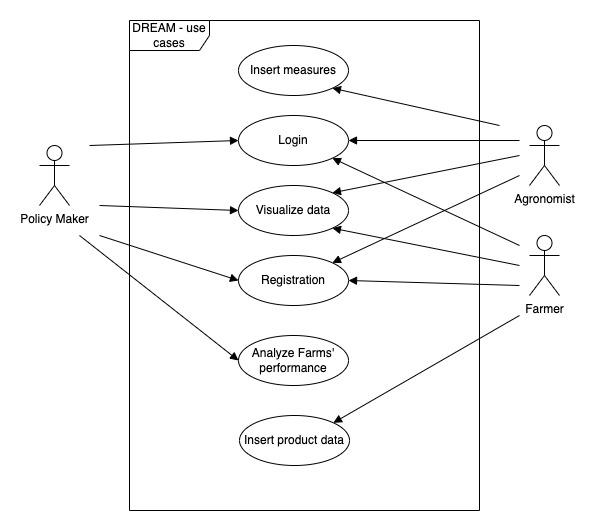
\includegraphics[width=350px]{UseCases diagrams/Use-Case-diagrams-Page-1.jpg}
    \caption{Use Case Diagram 1}
\end{figure}
\begin{figure}[H]
    \centering
    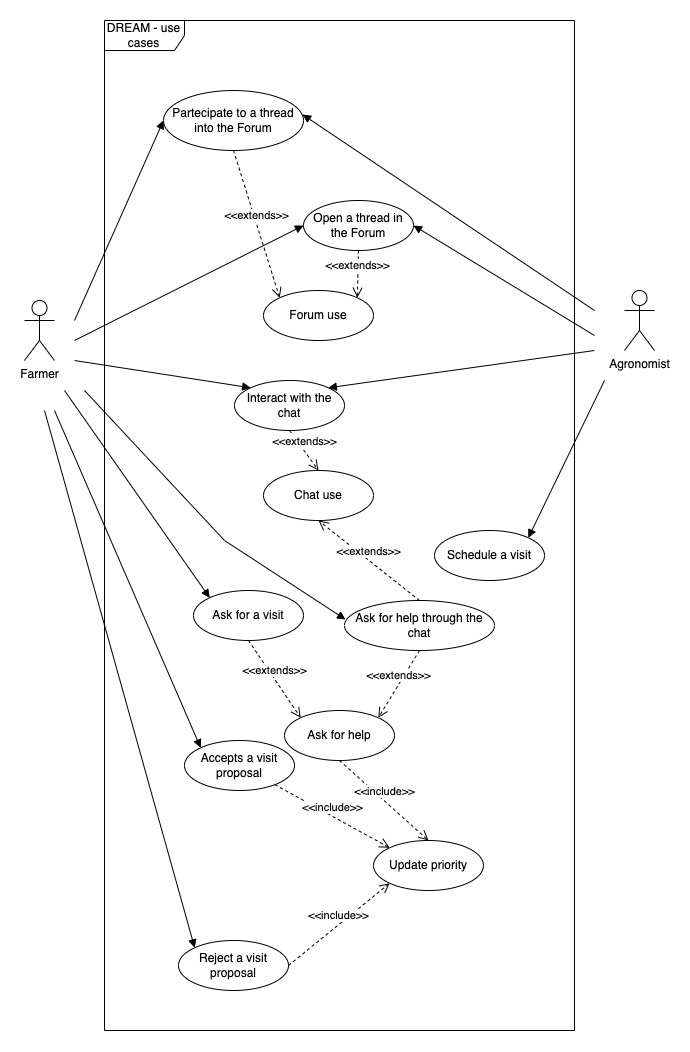
\includegraphics[width=350px]{UseCases diagrams/Use-Case-diagrams-Page-2.jpg}
    \caption{Use Case Diagram 2}
\end{figure}
\subsection{User's use cases}
\subsubsection{Use case 0.1: User Login}
\begin{longtable}[H]{ | l | p{10cm} | }
\hline
{\cellcolor[rgb]{0.753,0.753,0.753}}\textbf{ID}  & 0.1 \\ \hline
{\cellcolor[rgb]{0.753,0.753,0.753}}\textbf{Name} & User Login \\ \hline
{\cellcolor[rgb]{0.753,0.753,0.753}}\textbf{Actors} & User \\ \hline
{\cellcolor[rgb]{0.753,0.753,0.753}}\textbf{Entry conditions} &
\begin{itemize}
    \item The user is already registered
\end{itemize}
\\ \hline
{\cellcolor[rgb]{0.753,0.753,0.753}}\textbf{Input} & User's credentials \\ \hline
{\cellcolor[rgb]{0.753,0.753,0.753}}\textbf{Event flows} &
\begin{itemize}
    \item The user opens the application
    \item The user inserts their credentials
    \item The system checks the credentials
    \item The system lets the user login
\end{itemize}
\\ \hline
{\cellcolor[rgb]{0.753,0.753,0.753}}\textbf{Exit Condition} & The credentials are correct\\ \hline
{\cellcolor[rgb]{0.753,0.753,0.753}}\textbf{Output} & The user is logged in\\ \hline
{\cellcolor[rgb]{0.753,0.753,0.753}}\textbf{Exceptions} &
\begin{itemize}
    \item The credentials are wrong, therefore the system prevents the access
\end{itemize}
\\ \hline
\caption{Use case 0.1 - User login}
\\
\end{longtable}
\subsubsection{Use case 0.2: User visualizes data summary}
\begin{longtable}[H]{ | l | p{10cm} | }
\hline
{\cellcolor[rgb]{0.753,0.753,0.753}}\textbf{ID}  & 0.2 \\ \hline
{\cellcolor[rgb]{0.753,0.753,0.753}}\textbf{Name} & User visualizes data summary \\ \hline
{\cellcolor[rgb]{0.753,0.753,0.753}}\textbf{Actors} & User \\ \hline
{\cellcolor[rgb]{0.753,0.753,0.753}}\textbf{Entry conditions} &
\begin{itemize}
    \item The user has logged in the system
    \item The data are stored in the database
\end{itemize}
\\ \hline
{\cellcolor[rgb]{0.753,0.753,0.753}}\textbf{Input} & NULL \\ \hline
{\cellcolor[rgb]{0.753,0.753,0.753}}\textbf{Event flows} &
\begin{itemize}
    \item The user opens the application
    \item The user clicks on the button "Visualize data"
    \item The system shows the available data views
    \item The user selects the data views they are interested in
    \item The system checks if the user has the right permission to visualize data they are requiring
    \item The system fetches the required data
    \item The system displays the required data
\end{itemize}
\\ \hline
{\cellcolor[rgb]{0.753,0.753,0.753}}\textbf{Exit Condition} & Data are fetched and properly displayed\\ \hline
{\cellcolor[rgb]{0.753,0.753,0.753}}\textbf{Output} & Data summary is displayed\\ \hline
{\cellcolor[rgb]{0.753,0.753,0.753}}\textbf{Exceptions} &
\begin{itemize}
    \item The system fails to fetch data
    \item The user has not the right permissions to see the requested data
\end{itemize}
\\ \hline
\caption{Use case 0.2 - User visualizes data summary}
\\
\end{longtable}
\subsection{Farmer's use cases}
\subsubsection{Use case 1.1: Registration of a farmer}
\begin{longtable}[H]{ | l | p{10cm} | }
\hline
{\cellcolor[rgb]{0.753,0.753,0.753}}\textbf{ID}  & 1.1 \\ \hline
{\cellcolor[rgb]{0.753,0.753,0.753}}\textbf{Name} & Registration of the farmer \\ \hline
{\cellcolor[rgb]{0.753,0.753,0.753}}\textbf{Actors} & Farmer \\ \hline
{\cellcolor[rgb]{0.753,0.753,0.753}}\textbf{Entry conditions} &
\begin{itemize}
    \item The farmer is not already registered in the system
\end{itemize}
\\ \hline
{\cellcolor[rgb]{0.753,0.753,0.753}}\textbf{Input} & Farmer's credentials\\ \hline
{\cellcolor[rgb]{0.753,0.753,0.753}}\textbf{Event flows} &
\begin{itemize}
    \item The farmer opens the application
    \item The farmer clicks on the button "Sign Up"
    \item The system shows the registration form
    \item The farmer inserts their email and a password
    \item The system sends a confirmation email to the farmer
    \item The farmer confirms their email by clicking in the link received by email
    \item The system shows a form asking for the role of the farmer
    \item The farmer selects the option "Farmer"
    \item The system displays a form asking for data regarding the farmer's farm
    \item The farmer inserts data about their farm
    \item The system calculate the priority of the farm w.r.t. the list of farms belonging to the same area
    \item The system displays information about the area the farmer belongs to
    \item The system displays the list of agronomists the farmer will be able to reach
    \item The system sends a confirmation email to the farmer
\end{itemize}
\\ \hline
{\cellcolor[rgb]{0.753,0.753,0.753}}\textbf{Exit Condition} & Registration has been successful. The farmer's data is stored into the system's database. The farmer then will be able to login in the system by using their credentials.\\ \hline
{\cellcolor[rgb]{0.753,0.753,0.753}}\textbf{Output} & 
\begin{itemize}
    \item A verification email is sent to the farmer
    \item A confirmation email is sent to the farmer
\end{itemize}
\\ \hline
{\cellcolor[rgb]{0.753,0.753,0.753}}\textbf{Exceptions} &
\begin{itemize}
    \item The farmer is already registered into the system. The system then will prevent the user to register themselves twice.
    \item The farmer provides an invalid email. The farmer then will not be able to confirm their email.
\end{itemize}
\\ \hline
\caption{Use case 1.1 - Registration of the farmer}
\\
\end{longtable}
\subsubsection{Use case 1.2: Farmer asks help through the chat}
\begin{longtable}[H]{ | l | p{10cm} | }
\hline
{\cellcolor[rgb]{0.753,0.753,0.753}}\textbf{ID}  & 1.2 \\ \hline
{\cellcolor[rgb]{0.753,0.753,0.753}}\textbf{Name} & Farmer asks help through the chat \\ \hline
{\cellcolor[rgb]{0.753,0.753,0.753}}\textbf{Actors} & Farmer \\ \hline
{\cellcolor[rgb]{0.753,0.753,0.753}}\textbf{Entry conditions} &
\begin{itemize}
    \item The farmer needs help
    \item The farmer is already registered in the system
\end{itemize}
\\ \hline
{\cellcolor[rgb]{0.753,0.753,0.753}}\textbf{Input} & The farmer inserts a description of the problem they are facing\\ \hline
{\cellcolor[rgb]{0.753,0.753,0.753}}\textbf{Event flows} &
\begin{itemize}
    \item The farmer has a problem
    \item The farmer opens the application
    \item The farmer clicks on "Chat with an Agronomist"
    \item The system shows a form asking for information about the problem the farmer is facing
    \item The farmer inserts the required information
    \item The farmer clicks on "Send Request"
    \item The system acquires the data sent by the farmer
    \item The system confirms that the request has been successful
    \item The system shows, in the farmer interface, the request as "pending"
\end{itemize}
\\ \hline
{\cellcolor[rgb]{0.753,0.753,0.753}}\textbf{Exit Condition} & The request has been successfully sent to all the agronomists responsible of the area the farmer belongs to.\\ \hline
{\cellcolor[rgb]{0.753,0.753,0.753}}\textbf{Output} & 
\begin{itemize}
    \item The request is marked as "pending"
\end{itemize}
\\ \hline
{\cellcolor[rgb]{0.753,0.753,0.753}}\textbf{Exceptions} &
\begin{itemize}
    \item The farmer misses to fill one or more mandatory fields during the chat request. The system then will show an error such as "in order to open the chat request you need to fill up all the mandatory fields".
    \item The farmer closes the chat without clicking on "Send Request". By doing so the request is never sent but remains in the Farmer’s chat interface as a draft.
\end{itemize}
\\ \hline
\caption{Use case 1.2 - Farmer asks help through the chat}
\\
\end{longtable}
\subsubsection{Use case 1.3: Farmer asks for a visit}
\begin{longtable}[H]{ | l | p{10cm} | }
\hline
{\cellcolor[rgb]{0.753,0.753,0.753}}\textbf{ID}  & 1.3 \\ \hline
{\cellcolor[rgb]{0.753,0.753,0.753}}\textbf{Name} & Farmer asks for a visit \\ \hline
{\cellcolor[rgb]{0.753,0.753,0.753}}\textbf{Actors} & Farmer \\ \hline
{\cellcolor[rgb]{0.753,0.753,0.753}}\textbf{Entry conditions} &
\begin{itemize}
    \item The farmer needs help
    \item The farmer is already registered in the system
\end{itemize}
\\ \hline
{\cellcolor[rgb]{0.753,0.753,0.753}}\textbf{Input} & The farmer inserts a description of the problem they are facing\\ \hline
{\cellcolor[rgb]{0.753,0.753,0.753}}\textbf{Event flows} &
\begin{itemize}
    \item The farmer has a problem
    \item The farmer opens the application
    \item The farmer clicks on "Request a Visit"
    \item The system shows a form asking for information about the problem the farmer is facing
    \item The farmer inserts the required information
    \item The farmer clicks on "Send Request"
    \item The system acquires the data sent by the farmer
    \item The system updates the priority of the farm
    \item The system confirms that the request has been successful
    \item The system shows, in the farmer interface, the request as "pending"
\end{itemize}
\\ \hline
{\cellcolor[rgb]{0.753,0.753,0.753}}\textbf{Exit Condition} & The priority of the farm is updated. putting it on top of the list of farms belonging to the same area. Moreover the farm is marked in such a way that agronomists will be able to notice that the farmer has requested a visit.\\ \hline
{\cellcolor[rgb]{0.753,0.753,0.753}}\textbf{Output} & 
The priority of the farm is updated putting it on top of the list of farms belonging to the same area. Moreover the farm is marked in such a way that agronomists will be able to notice that the farmer has requested a visit.
\\ \hline
{\cellcolor[rgb]{0.753,0.753,0.753}}\textbf{Exceptions} &
\begin{itemize}
    \item The farmer misses to fill one or more mandatory fields during the chat request. The system then will show an error such as ""in order to open the chat request you need to fill up all the mandatory fields.
    \item The farmer closes the chat without clicking on "Send Request". By doing so the request is never sent but remains in the Farmer’s chat interface as a draft.
\end{itemize}
\\ \hline
\caption{Use case 1.3 - Farmer asks for a visit}
\\
\end{longtable}
\subsubsection{Use case 1.4: Farmer accepts a visit proposal}
\begin{longtable}[H]{ | l | p{10cm} | }
\hline
{\cellcolor[rgb]{0.753,0.753,0.753}}\textbf{ID}  & 1.4 \\ \hline
{\cellcolor[rgb]{0.753,0.753,0.753}}\textbf{Name} & Farmer accepts a visit proposal \\ \hline
{\cellcolor[rgb]{0.753,0.753,0.753}}\textbf{Actors} & Farmer \\ \hline
{\cellcolor[rgb]{0.753,0.753,0.753}}\textbf{Entry conditions} &
\begin{itemize}
    \item An agronomist scheduled a visit to the farmer's farm
    \item The farmer is already registered in the system
\end{itemize}
\\ \hline
{\cellcolor[rgb]{0.753,0.753,0.753}}\textbf{Input} & Visit proposal by an agronomist\\ \hline
{\cellcolor[rgb]{0.753,0.753,0.753}}\textbf{Event flows} &
\begin{itemize}
    \item The system notifies the farmer that there is a visit proposal
    \item The farmer taps on the notification
    \item The farmer clicks on "Request a Visit"
    \item The system shows details about the proposed visit, such as the date and the time of the visit
    \item The farmer accepts the visit by clicking on the "Confirm" button
    \item The system shows both to the farmer and to the agronomist that the visit has been scheduled
\end{itemize}
\\ \hline
{\cellcolor[rgb]{0.753,0.753,0.753}}\textbf{Exit Condition} & The farmer accepts the proposed visit.\\ \hline
{\cellcolor[rgb]{0.753,0.753,0.753}}\textbf{Output} & 
\begin{itemize}
    \item A notification is sent on the agronomist's device.
    \item A notification is sent on the farmer's device.
\end{itemize}
\\ \hline
{\cellcolor[rgb]{0.753,0.753,0.753}}\textbf{Exceptions} & The farmer does not confirm nor rejects the proposed visit. In this case the system should continue pushing the notification containing the proposed visit.
\\ \hline
\caption{Use case 1.4 - Farmer accepts a visit proposal}
\\
\end{longtable}
\subsubsection{Use case 1.5: Farmer rejects a visit proposal}
\begin{longtable}[H]{ | l | p{10cm} | }
\hline
{\cellcolor[rgb]{0.753,0.753,0.753}}\textbf{ID}  & 1.5 \\ \hline
{\cellcolor[rgb]{0.753,0.753,0.753}}\textbf{Name} & Farmer rejects a visit proposal \\ \hline
{\cellcolor[rgb]{0.753,0.753,0.753}}\textbf{Actors} & Farmer \\ \hline
{\cellcolor[rgb]{0.753,0.753,0.753}}\textbf{Entry conditions} &
\begin{itemize}
    \item An agronomist scheduled a visit to the farmer's farm
    \item The farmer is already registered in the system
\end{itemize}
\\ \hline
{\cellcolor[rgb]{0.753,0.753,0.753}}\textbf{Input} & Visit proposal by an agronomist\\ \hline
{\cellcolor[rgb]{0.753,0.753,0.753}}\textbf{Event flows} &
\begin{itemize}
    \item The system notifies the farmer that there is a visit proposal
    \item The farmer taps on the notification
    \item The farmer clicks on "Request a Visit"
    \item The system shows details about the proposed visit, such as the date and the time of the visit
    \item The farmer rejects the visit by clicking on the "Reject" button
    \item The system shows the farmer a form asking to propose new dates for the visit
    \item The farmer selects new dates and clicks on "Propose Dates"
    \item The system confirms the farmer that the dates have been forwarded to the agronomist
    \item The system notifies the agronomist about the rejection and shows them the new proposed dates
\end{itemize}
\\ \hline
{\cellcolor[rgb]{0.753,0.753,0.753}}\textbf{Exit Condition} & The agronomist is notified that the farmer has rejected the visit\\ \hline
{\cellcolor[rgb]{0.753,0.753,0.753}}\textbf{Output} & 
\begin{itemize}
    \item A notification is sent on the agronomist's device.
    \item A notification is sent on the farmer's device.
\end{itemize}
\\ \hline
{\cellcolor[rgb]{0.753,0.753,0.753}}\textbf{Exceptions} & 
\begin{itemize}
    \item The farmer tries to reject the upcoming visit on the same day of the visit which is forbidden by the system
    \item The farmer does not confirm nor rejects the proposed visit. In this case the system should continue pushing the notification containing the proposed visit.
\end{itemize}
\\ \hline
\caption{Use case 1.5 - Farmer rejects a visit proposal}
\\
\end{longtable}
\subsubsection{Use case 1.6: Farmer and Agronomist interact through the chat}
\begin{longtable}[H]{ | l | p{10cm} | }
\hline
{\cellcolor[rgb]{0.753,0.753,0.753}}\textbf{ID}  & 1.6 \\ \hline
{\cellcolor[rgb]{0.753,0.753,0.753}}\textbf{Name} & Farmer and Agronomist interact through the chat \\ \hline
{\cellcolor[rgb]{0.753,0.753,0.753}}\textbf{Actors} & Farmer and Agronomist \\ \hline
{\cellcolor[rgb]{0.753,0.753,0.753}}\textbf{Entry conditions} &
\begin{itemize}
    \item The farmer has an open chat with an agronomist
    \item The farmer is already registered in the system
\end{itemize}
\\ \hline
{\cellcolor[rgb]{0.753,0.753,0.753}}\textbf{Input} & Messages in the chat\\ \hline
{\cellcolor[rgb]{0.753,0.753,0.753}}\textbf{Event flows} &
\begin{itemize}
    \item The notification "A chat has been opened" is received by the farmer
    \item The farmer taps on the notification
    \item The system shows the farmer the first message written by the agronomist
    \item The farmer reads the answer and in case there are more doubt they can keep asking questions using the chat
    \item The system notifies the agronomist that one ore more messages have been written in the chat
    \item The agronomist taps on the notification
    \item The system shows the agronomist the new messages
    \item The agronomist reads the new messages and replies to them
    \item ...
    \item When the conversation is over the agronomist send a request to close the chat
    \item The system notifies the farmer that the agronomist wants to close the chat
    \item The farmer approves the action of the agronomist by clicking on "Confirm"
    \item The system closes the chat
    \item The system saves the chat history in its databases
\end{itemize}
\\ \hline
{\cellcolor[rgb]{0.753,0.753,0.753}}\textbf{Exit Condition} & The farmer gets all the answer they needed from the agronomist, which, therefore, proposes to close the chat\\ \hline
{\cellcolor[rgb]{0.753,0.753,0.753}}\textbf{Output} & 
Chat history
\\ \hline
{\cellcolor[rgb]{0.753,0.753,0.753}}\textbf{Exceptions} & 
The agronomist proposes to close the chat, but the farmer ignores the notification. In this case the system closes the chat automatically in 24h. 
\\ \hline
\caption{Use case 1.6 - Farmer and Agronomist interact through the chat}
\\
\end{longtable}
\subsubsection{Use case 1.7: Farmer opens a thread in the forum}
\begin{longtable}[H]{ | l | p{10cm} | }
\hline
{\cellcolor[rgb]{0.753,0.753,0.753}}\textbf{ID}  & 1.7 \\ \hline
{\cellcolor[rgb]{0.753,0.753,0.753}}\textbf{Name} & Farmer opens a thread in the forum \\ \hline
{\cellcolor[rgb]{0.753,0.753,0.753}}\textbf{Actors} & Farmer \\ \hline
{\cellcolor[rgb]{0.753,0.753,0.753}}\textbf{Entry conditions} &
\begin{itemize}
    \item The farmer wants to share some thoughts
    \item The farmer is already registered in the system
\end{itemize}
\\ \hline
{\cellcolor[rgb]{0.753,0.753,0.753}}\textbf{Input} & Title of the thread and description of the thread\\ \hline
{\cellcolor[rgb]{0.753,0.753,0.753}}\textbf{Event flows} &
\begin{itemize}
    \item The farmer opens the application
    \item The farmer clicks on the "Forum" button
    \item The system display the screen relative to the forum
    \item The farmer taps on the button "Open a Thread"
    \item The system displays a forum asking for a title for the thread and the description of the thread
    \item The farmer fills up the fields
    \item The farmer clicks on the "Confirm" button
    \item The system opens the required thread
    \item The system shows the new thread to all the farmer which navigate through the forum
\end{itemize}
\\ \hline
{\cellcolor[rgb]{0.753,0.753,0.753}}\textbf{Exit Condition} & The farmer successfully publish their new thread on the forum\\ \hline
{\cellcolor[rgb]{0.753,0.753,0.753}}\textbf{Output} & 
The system have a new thread
\\ \hline
{\cellcolor[rgb]{0.753,0.753,0.753}}\textbf{Exceptions} & 
\begin{itemize}
    \item The title of the thread provided by the farmer has already been used
    \item The farmer closes the application before clicking the "Confirm" button. By doing so all the content are saved as draft for the next time the farmer wants to open a new thread 

\end{itemize}
\\ \hline
\caption{Use case 1.7 - Farmer opens a thread in the forum}
\\
\end{longtable}
\subsubsection{Use case 1.8: Farmer participates to a thread in a forum}
\begin{longtable}[H]{ | l | p{10cm} | }
\hline
{\cellcolor[rgb]{0.753,0.753,0.753}}\textbf{ID}  & 1.8 \\ \hline
{\cellcolor[rgb]{0.753,0.753,0.753}}\textbf{Name} & Farmer participates to a thread in a forum \\ \hline
{\cellcolor[rgb]{0.753,0.753,0.753}}\textbf{Actors} & Farmer \\ \hline
{\cellcolor[rgb]{0.753,0.753,0.753}}\textbf{Entry conditions} & The farmer is already registered in the system \\ \hline
{\cellcolor[rgb]{0.753,0.753,0.753}}\textbf{Input} & A message sent by the farmer\\ \hline
{\cellcolor[rgb]{0.753,0.753,0.753}}\textbf{Event flows} &
\begin{itemize}
    \item The farmer opens the application
    \item The farmer clicks on the "Forum" button
    \item The system display the screen relative to the forum, and in particular the list of all the thread order by the most recent to the least recent 
    \item The farmer selects a thread
    \item The system displays all the messages belonging to the thread and the form used to append new messages to the thread itself
    \item The farmer appends a message to the thread 
    \item The farmer clicks on the "Comment" button
    \item The system appends the new message to the thread
\end{itemize}
\\ \hline
{\cellcolor[rgb]{0.753,0.753,0.753}}\textbf{Exit Condition} & The farmer successfully publish their message into the thread\\ \hline
{\cellcolor[rgb]{0.753,0.753,0.753}}\textbf{Output} & 
The thread has a new message in it
\\ \hline
{\cellcolor[rgb]{0.753,0.753,0.753}}\textbf{Exceptions} & The Farmer closes the application before clicking the "Comment" button. By doing so all the content is lost.
\\ \hline
\caption{Use case 1.8 - Farmer participates to a thread in a forum}
\\
\end{longtable}
\subsubsection{Use case 1.9: Farmer inserts data about production}
\begin{longtable}[H]{ | l | p{10cm} | }
\hline
{\cellcolor[rgb]{0.753,0.753,0.753}}\textbf{ID}  & 1.9 \\ \hline
{\cellcolor[rgb]{0.753,0.753,0.753}}\textbf{Name} & Farmer inserts data about production \\ \hline
{\cellcolor[rgb]{0.753,0.753,0.753}}\textbf{Actors} & Farmer \\ \hline
{\cellcolor[rgb]{0.753,0.753,0.753}}\textbf{Entry conditions} &
\begin{itemize}
    \item The farmer is already registered in the system
    \item The farmer has already done the harvest
\end{itemize}
\\ \hline
{\cellcolor[rgb]{0.753,0.753,0.753}}\textbf{Input} & Farm's production data\\ \hline
{\cellcolor[rgb]{0.753,0.753,0.753}}\textbf{Event flows} &
\begin{itemize}
    \item The farmer opens the application
    \item The farmer clicks on the "Production Data" button
    \item The system display a form asking for information about the latest harvest 
    \item The farmer fills up the form with data relative to their production
    \item The farmer clicks on the "Confirm" button
    \item The system stores the data inside a database
    \item The system updates the priority of the farm
\end{itemize}
\\ \hline
{\cellcolor[rgb]{0.753,0.753,0.753}}\textbf{Exit Condition} & The farmer successfully inserts the data regarding their production\\ \hline
{\cellcolor[rgb]{0.753,0.753,0.753}}\textbf{Output} & NULL
\\ \hline
{\cellcolor[rgb]{0.753,0.753,0.753}}\textbf{Exceptions} & The Farmer closes the application before clicking the "Confirm" button. By doing so all the content is lost.
\\ \hline
\caption{Use case 1.9 - Farmer inserts data about production}
\\
\end{longtable}
\subsection{Agronomist's use cases}
\subsubsection{Use case 2.1: Registration of the agronomist}
\begin{longtable}[H]{ | l | p{10cm} | }
\hline
{\cellcolor[rgb]{0.753,0.753,0.753}}\textbf{ID}  & 2.1 \\ \hline
{\cellcolor[rgb]{0.753,0.753,0.753}}\textbf{Name} & Registration of the agronomist \\ \hline
{\cellcolor[rgb]{0.753,0.753,0.753}}\textbf{Actors} & Agronomist \\ \hline
{\cellcolor[rgb]{0.753,0.753,0.753}}\textbf{Entry conditions} &
\begin{itemize}
    \item The agronomist is not already registered in the system
\end{itemize}
\\ \hline
{\cellcolor[rgb]{0.753,0.753,0.753}}\textbf{Input} & Agronomist's credentials\\ \hline
{\cellcolor[rgb]{0.753,0.753,0.753}}\textbf{Event flows} &
\begin{itemize}
    \item The agronomist opens the application
    \item The agronomist clicks on the button "Sign Up"
    \item The system shows the registration form
    \item The agronomist inserts their email and a password
    \item The system sends a confirmation email to the agronomist
    \item The agronomist confirms their email by clicking in the link received by email
    \item The system shows a form asking for the role of the agronomist
    \item The farmer selects the option "Agronomist"
    \item The system displays a form asking for data regarding the agronomist; in particular, among the others, the are in which they work in
    \item The agronomist fills the form with the required data
    \item The system displays information about the area the agronomist belongs to
    \item The system displays the list of farm the agronomist will be responsible of
    \item The system sends a confirmation email to the farmer
\end{itemize}
\\ \hline
{\cellcolor[rgb]{0.753,0.753,0.753}}\textbf{Exit Condition} & Registration has been successful. The agronomist's data is stored into the system's database. The agronomist then will be able to login in the system by using their credentials.\\ \hline
{\cellcolor[rgb]{0.753,0.753,0.753}}\textbf{Output} & 
\begin{itemize}
    \item A verification email is sent to the agronomist
    \item A confirmation email is sent to the agronomist
\end{itemize}
\\ \hline
{\cellcolor[rgb]{0.753,0.753,0.753}}\textbf{Exceptions} &
\begin{itemize}
    \item The agronomist is already registered into the system. The system then will prevent the user to register themselves twice.
    \item The agronomist provides an invalid email. The agronomist then will not be able to confirm their email.
\end{itemize}
\\ \hline
\caption{Use case 2.1 - Registration of the agronomist}
\\
\end{longtable}
\subsubsection{Use case 2.2: Agronomist takes charge of a chat request}
\begin{longtable}[H]{ | l | p{10cm} | }
\hline
{\cellcolor[rgb]{0.753,0.753,0.753}}\textbf{ID}  & 2.2 \\ \hline
{\cellcolor[rgb]{0.753,0.753,0.753}}\textbf{Name} & Agronomist takes charge of a chat request \\ \hline
{\cellcolor[rgb]{0.753,0.753,0.753}}\textbf{Actors} & Agronomist \\ \hline
{\cellcolor[rgb]{0.753,0.753,0.753}}\textbf{Entry conditions} &
\begin{itemize}
    \item The agronomist has a chat request pending
    \item The request has been issued by a farmer that belongs to the same area of the agronomist
    \item The agronomist is already registered in the system
    \item The agronomist has logged in the system
\end{itemize}
\\ \hline
{\cellcolor[rgb]{0.753,0.753,0.753}}\textbf{Input} & A message from the agronomist\\ \hline
{\cellcolor[rgb]{0.753,0.753,0.753}}\textbf{Event flows} &
\begin{itemize}
    \item The system notifies the agronomist that a farmer has requested to chat with them
    \item The agronomist taps on the notification
    \item The system shows the agronomist the list of pending chat requests
    \item The agronomist selects a chat request and clicks on "Process request"
    \item The system opens a chat between the farmer who requested it and the agronomist
    \item The notifies shows both to the farmer and to the agronomist that the chat is open
    \item The agronomist writes the first message in the chat
\end{itemize}
\\ \hline
{\cellcolor[rgb]{0.753,0.753,0.753}}\textbf{Exit Condition} & The chat is opened.\\ \hline
{\cellcolor[rgb]{0.753,0.753,0.753}}\textbf{Output} & There exists a chat between the agronomist and the farmer\\ \hline
{\cellcolor[rgb]{0.753,0.753,0.753}}\textbf{Exceptions} &
\begin{itemize}
    \item The agronomist closes the chat before clicking on “Process request”, so the chat request is still “pending”
    \item The agronomist clicks on “Process request” but in the meanwhile the request was opened by another agronomist in the same area. The system shows them an error message: “This chat request is already opened by another agronomist”
\end{itemize}
\\ \hline
\caption{Use case 2.2 - Agronomist takes charge of a chat request}
\\
\end{longtable}
\subsubsection{Use case 2.3: Agronomist schedules a visit to a farm}
\begin{longtable}[H]{ | l | p{10cm} | }
\hline
{\cellcolor[rgb]{0.753,0.753,0.753}}\textbf{ID}  & 2.3 \\ \hline
{\cellcolor[rgb]{0.753,0.753,0.753}}\textbf{Name} & Agronomist schedules a visit to a farm\\ \hline
{\cellcolor[rgb]{0.753,0.753,0.753}}\textbf{Actors} & Agronomist \\ \hline
{\cellcolor[rgb]{0.753,0.753,0.753}}\textbf{Entry conditions} &
\begin{itemize}
    \item The agronomist has is registered in the system
    \item The agronomist has logged in
    \item The agronomist wants to add a visit to their schedule
\end{itemize}
\\ \hline
{\cellcolor[rgb]{0.753,0.753,0.753}}\textbf{Input} & NULL \\ \hline
{\cellcolor[rgb]{0.753,0.753,0.753}}\textbf{Event flows} &
\begin{itemize}
    \item The agronomist opens the application
    \item The system shows the agronomist their dashboard
    \item The agronomist taps on the "Farms List" button
    \item The system shows the list of the farms, that belong to the area of the agronomist, ordered by priority and possibly marked if the farmer requested a visit
    \item The agronomist selects the top farm and clicks on "Schedule a visit"
    \item The system opens the schedule of the agronomist and asks them when they want to visit the selected farm
    \item The agronomist selects the date and the time in which they want to visit the farm
    \item The agronomist clicks on "Confirm"
    \item The system updates the agronomist’s schedule adding this visit
    \item The system sends the information about the upcoming visit to the farmer
\end{itemize}
\\ \hline
{\cellcolor[rgb]{0.753,0.753,0.753}}\textbf{Exit Condition} & The visit has been successfully inserted in the agronomist’s schedule, and the details have been successfully sent to the farmer.\\ \hline
{\cellcolor[rgb]{0.753,0.753,0.753}}\textbf{Output} & The relative farmer is notified that there is an upcoming visit scheduled\\ \hline
{\cellcolor[rgb]{0.753,0.753,0.753}}\textbf{Exceptions} &
The agronomist closes the chat before clicking on "Confirm". In this case the visit is not scheduled and the notification to the farmer is not sent.
\\ \hline
\caption{Use case 2.3 - Agronomist schedules a visit to a farm}
\\
\end{longtable}
\subsubsection{Use case 2.4: Agronomist confirms a scheduled visit}
\begin{longtable}[H]{ | l | p{10cm} | }
\hline
{\cellcolor[rgb]{0.753,0.753,0.753}}\textbf{ID}  & 2.4 \\ \hline
{\cellcolor[rgb]{0.753,0.753,0.753}}\textbf{Name} & Agronomist confirms a scheduled visit\\ \hline
{\cellcolor[rgb]{0.753,0.753,0.753}}\textbf{Actors} & Agronomist \\ \hline
{\cellcolor[rgb]{0.753,0.753,0.753}}\textbf{Entry conditions} &
\begin{itemize}
    \item The agronomist has logged in
\end{itemize}
\\ \hline
{\cellcolor[rgb]{0.753,0.753,0.753}}\textbf{Input} &
\begin{itemize}
    \item The daily schedule of the agronomist
    \item A visit that the agronomist has completed
\end{itemize}
\\ \hline
{\cellcolor[rgb]{0.753,0.753,0.753}}\textbf{Event flows} &
\begin{itemize}
    \item The agronomist opens the application
    \item The system shows the agronomist their dashboard
    \item The agronomist taps on the "Schedule" button
    \item The system shows the agronomist their daily schedule
    \item The agronomist selects a visit and confirms it by clicking on "Done"
    \item The system shows a form that allows the agronomist to insert data about measurements taken during the visit and a report of the visit. The report of the visit is marked as mandatory.
    \item The agronomist fills in the form
    \item The agronomist clicks on "Confirm"
    \item The system stores the data in the database
\end{itemize}
\\ \hline
{\cellcolor[rgb]{0.753,0.753,0.753}}\textbf{Exit Condition} & The system has updated the schedule with the confirmed visit and it has stored the data concerning the confirmed visit.\\ \hline
{\cellcolor[rgb]{0.753,0.753,0.753}}\textbf{Output} & 
\begin{itemize}
    \item The report of the visit
    \item (Optional) Data about measurements taken by the agronomist
\end{itemize}
\\ \hline
{\cellcolor[rgb]{0.753,0.753,0.753}}\textbf{Exceptions} &
The agronomist does not fill the report field of the form, thus it is impossible to confirm the visit
\\ \hline
\caption{Use case 2.4 - Agronomist confirms a scheduled visit}
\\
\end{longtable}
\subsubsection{Use case 2.5: Agronomist cancels a scheduled visit}
\begin{longtable}[H]{ | l | p{10cm} | }
\hline
{\cellcolor[rgb]{0.753,0.753,0.753}}\textbf{ID}  & 2.5 \\ \hline
{\cellcolor[rgb]{0.753,0.753,0.753}}\textbf{Name} & Agronomist cancels a scheduled visit\\ \hline
{\cellcolor[rgb]{0.753,0.753,0.753}}\textbf{Actors} & Agronomist \\ \hline
{\cellcolor[rgb]{0.753,0.753,0.753}}\textbf{Entry conditions} &
\begin{itemize}
    \item The agronomist has logged in
\end{itemize}
\\ \hline
{\cellcolor[rgb]{0.753,0.753,0.753}}\textbf{Input} &
\begin{itemize}
    \item The daily schedule of the agronomist
    \item A visit that the agronomist can not attend
\end{itemize}
\\ \hline
{\cellcolor[rgb]{0.753,0.753,0.753}}\textbf{Event flows} &
\begin{itemize}
    \item The agronomist opens the application
    \item The system shows the agronomist their dashboard
    \item The agronomist taps on the "Schedule" button
    \item The system shows the agronomist their schedule
    \item The agronomist selects a visit and cancels it by clicking on "Cancel"
    \item The system shows a form that allows the agronomist to send a message to the farmer in order to explain why the visit can not take place as scheduled.
    \item The agronomist fills in the form
    \item The agronomist clicks on "Confirm"
    \item The system notifies the farmer about the cancelled visit
\end{itemize}
\\ \hline
{\cellcolor[rgb]{0.753,0.753,0.753}}\textbf{Exit Condition} &
\begin{itemize}
    \item The system has updated the schedule considering the canceled visit
    \item The farmer is notified that the scheduled visit has been canceled
\end{itemize}
\\ \hline
{\cellcolor[rgb]{0.753,0.753,0.753}}\textbf{Output} & A notification is sent to the farmer.
\\ \hline
{\cellcolor[rgb]{0.753,0.753,0.753}}\textbf{Exceptions} &
The agronomist tries to cancel a visit that is already confirmed. The system forbids the operation.
\\ \hline
\caption{Use case 2.5 - Agronomist cancels a scheduled visit}
\\
\end{longtable}
\subsubsection{Use case 2.6: Agronomist opens a thread in the forum}
\begin{longtable}[H]{ | l | p{10cm} | }
\hline
{\cellcolor[rgb]{0.753,0.753,0.753}}\textbf{ID}  & 2.6 \\ \hline
{\cellcolor[rgb]{0.753,0.753,0.753}}\textbf{Name} & Agronomist opens a thread in the forum \\ \hline
{\cellcolor[rgb]{0.753,0.753,0.753}}\textbf{Actors} & Agronomist \\ \hline
{\cellcolor[rgb]{0.753,0.753,0.753}}\textbf{Entry conditions} &
\begin{itemize}
    \item The agronomist wants to share some thoughts
    \item The agronomist is already registered in the system
\end{itemize}
\\ \hline
{\cellcolor[rgb]{0.753,0.753,0.753}}\textbf{Input} & Title of the thread and description of the thread\\ \hline
{\cellcolor[rgb]{0.753,0.753,0.753}}\textbf{Event flows} &
\begin{itemize}
    \item The agronomist opens the application
    \item The agronomist clicks on the "Forum" button
    \item The system display the screen relative to the forum
    \item The agronomist taps on the button "Open a Thread"
    \item The system displays a forum asking for a title for the thread and the description of the thread
    \item The agronomist fills up the fields
    \item The agronomist clicks on the "Confirm" button
    \item The system opens the required thread
    \item The system shows the new thread to all the agronomist which navigate through the forum
\end{itemize}
\\ \hline
{\cellcolor[rgb]{0.753,0.753,0.753}}\textbf{Exit Condition} & The agronomist successfully publish their new thread on the forum\\ \hline
{\cellcolor[rgb]{0.753,0.753,0.753}}\textbf{Output} & 
The system have a new thread
\\ \hline
{\cellcolor[rgb]{0.753,0.753,0.753}}\textbf{Exceptions} & 
\begin{itemize}
    \item The title of the thread provided by the agronomist has already been used
    \item The agronomist closes the application before clicking the "Confirm" button. By doing so all the content are saved as draft for the next time the agronomist wants to open a new thread 

\end{itemize}
\\ \hline
\caption{Use case 2.6 - Agronomist opens a thread in the forum}
\\
\end{longtable}
\subsubsection{Use case 2.7: Agronomist participates to a thread in a forum}
\begin{longtable}[H]{ | l | p{10cm} | }
\hline
{\cellcolor[rgb]{0.753,0.753,0.753}}\textbf{ID}  & 2.7 \\ \hline
{\cellcolor[rgb]{0.753,0.753,0.753}}\textbf{Name} & Agronomist participates to a thread in a forum \\ \hline
{\cellcolor[rgb]{0.753,0.753,0.753}}\textbf{Actors} & Agronomist \\ \hline
{\cellcolor[rgb]{0.753,0.753,0.753}}\textbf{Entry conditions} & The agronomist is already registered in the system \\ \hline
{\cellcolor[rgb]{0.753,0.753,0.753}}\textbf{Input} & A message sent by the agronomist\\ \hline
{\cellcolor[rgb]{0.753,0.753,0.753}}\textbf{Event flows} &
\begin{itemize}
    \item The agronomist opens the application
    \item The agronomist clicks on the "Forum" button
    \item The system display the screen relative to the forum, and in particular the list of all the thread order by the most recent to the least recent 
    \item The agronomist selects a thread
    \item The system displays all the messages belonging to the thread and the form used to append new messages to the thread itself
    \item The agronomist appends a message to the thread 
    \item The agronomist clicks on the "Comment" button
    \item The system appends the new message to the thread
\end{itemize}
\\ \hline
{\cellcolor[rgb]{0.753,0.753,0.753}}\textbf{Exit Condition} & The agronomist successfully publish their message into the thread\\ \hline
{\cellcolor[rgb]{0.753,0.753,0.753}}\textbf{Output} & 
The thread has a new message in it
\\ \hline
{\cellcolor[rgb]{0.753,0.753,0.753}}\textbf{Exceptions} & The Agronomist closes the application before clicking the "Comment" button. By doing so all the content is lost.
\\ \hline
\caption{Use case 2.7- Agronomist participates to a thread in a forum}
\\
\end{longtable}
\subsection{Policy Maker's use cases}
\subsubsection{Use case 3.1: Registration of the Policy Maker}
\begin{longtable}[H]{ | l | p{10cm} | }
\hline
{\cellcolor[rgb]{0.753,0.753,0.753}} \textbf{ID}  & 3.1 \\ \hline
{\cellcolor[rgb]{0.753,0.753,0.753}} \textbf{Name} & Registration of the Policy Maker \\ \hline
{\cellcolor[rgb]{0.753,0.753,0.753}}\textbf{Actors} & Policy Maker \\ \hline
{\cellcolor[rgb]{0.753,0.753,0.753}}\textbf{Entry conditions} & The policy maker is not already registered in the system \\ \hline
{\cellcolor[rgb]{0.753,0.753,0.753}}\textbf{Input} & Policy maker's credentials \\ \hline
{\cellcolor[rgb]{0.753,0.753,0.753}}\textbf{Event flows} &
\begin{itemize}
    \item The policy maker opens the application
    \item The policy maker clicks on the button "Sign Up"
    \item The system shows the registration form
    \item The policy maker inserts their email and a password
    \item The system sends a confirmation email to the policy maker
    \item The policy maker confirms their email by clicking in the link received by email
    \item The system shows a form asking for the role of the policy maker
    \item The farmer selects the option "Policy maker"
    \item The system shows a form asking for the personal information used in order to identify the policy maker
    \item The policy maker inserts the requested data
    \item The system sends a confirmation email to the Policy Maker
\end{itemize}
\\ \hline
{\cellcolor[rgb]{0.753,0.753,0.753}}\textbf{Exit Condition} & Registration has been successful. The farmer's data is stored into the system's database. The policy maker then will be able to login in the system by using their credentials.\\ \hline
{\cellcolor[rgb]{0.753,0.753,0.753}}\textbf{Output} & 
\begin{itemize}
    \item A verification email is sent to the Policy Maker
    \item A confirmation email is sent to the Policy Maker
\end{itemize}
\\ \hline
{\cellcolor[rgb]{0.753,0.753,0.753}}\textbf{Exceptions} &
\begin{itemize}
    \item The Policy Maker is already registered into the system. The system then will prevent the user to register themselves twice.
    \item The Policy Maker provides an invalid email. The Policy Maker then will not be able to confirm their email.
\end{itemize}
\\ \hline
\caption{Use case 3.1 - Registration of the Policy Maker}
\\
\end{longtable}
\subsubsection{Use case 3.2: Policy Makers analyze farmer’s performance}
\begin{longtable}[H]{ | l | p{10cm} | }
\hline
{\cellcolor[rgb]{0.753,0.753,0.753}}\textbf{ID}  & 3.2 \\ \hline
{\cellcolor[rgb]{0.753,0.753,0.753}}\textbf{Name} & Policy Makers analyze farmer’s performance  \\ \hline
{\cellcolor[rgb]{0.753,0.753,0.753}}\textbf{Actors} & Policy Maker \\ \hline
{\cellcolor[rgb]{0.753,0.753,0.753}}\textbf{Entry conditions} &
\begin{itemize}
    \item The Policy Maker has already logged in the system
    \item The data are stored in the database
    \item The machine learning techniques have to be already defined
\end{itemize}
\\ \hline
{\cellcolor[rgb]{0.753,0.753,0.753}}\textbf{Input} & NULL\\ \hline
{\cellcolor[rgb]{0.753,0.753,0.753}}\textbf{Event flows} &
\begin{itemize}
    \item The Policy Maker clicks on "Compute Performance" data summary
    \item The system computes the rank of the best farms using machine learning techniques already defined
    \item The system shows the ranking computed before 
\end{itemize}
\\ \hline
{\cellcolor[rgb]{0.753,0.753,0.753}}\textbf{Exit Condition} & The data are fetched and properly displayed\\ \hline
{\cellcolor[rgb]{0.753,0.753,0.753}}\textbf{Output} & 
The ranking built.
\\ \hline
{\cellcolor[rgb]{0.753,0.753,0.753}}\textbf{Exceptions} &
The system fails to fetch the data.
\\ \hline
\caption{Use case 3.2 - Policy Makers analyze farmer’s performance}
\\
\end{longtable}
\subsection{Activity Diagrams}
\subsubsection{Activity Diagram: User Registration}
The following three activity diagrams maps the use case tables 1.1, 2.1, 3.1 respectively.
\begin{figure}[H]
    \centering
    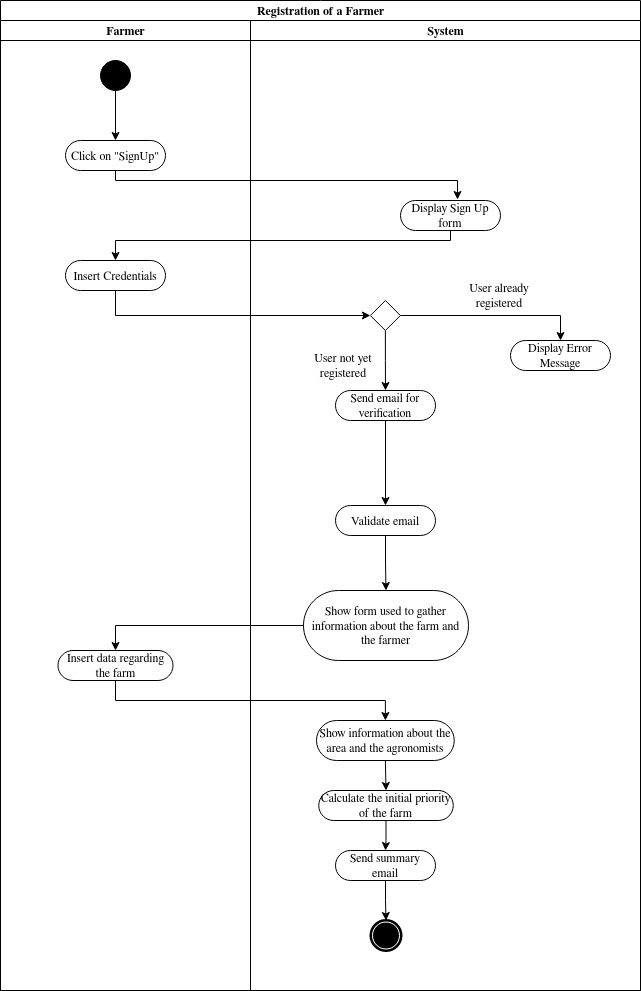
\includegraphics[width=250px]{ActivityDiagrams/FarmerSignUp.jpg}
    \caption{Activity diagram: Farmer Sign Up}
\end{figure}
\begin{figure}[H]
    \centering
    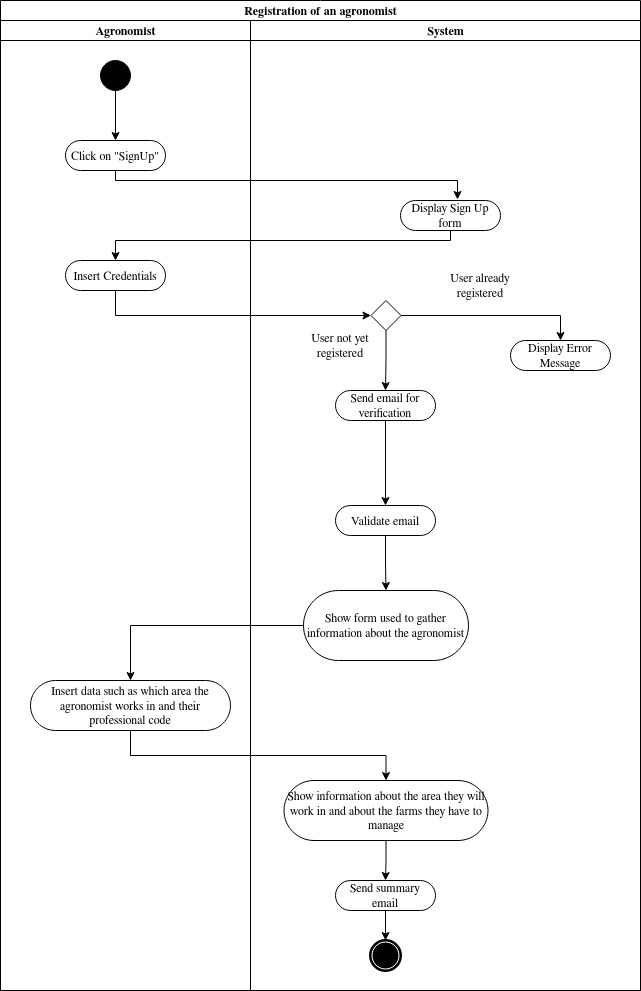
\includegraphics[width=250px]{ActivityDiagrams/AgronomistSignUp.jpg}
    \caption{Activity diagram: Agronomist Sign Up}
\end{figure}
\begin{figure}[H]
    \centering
    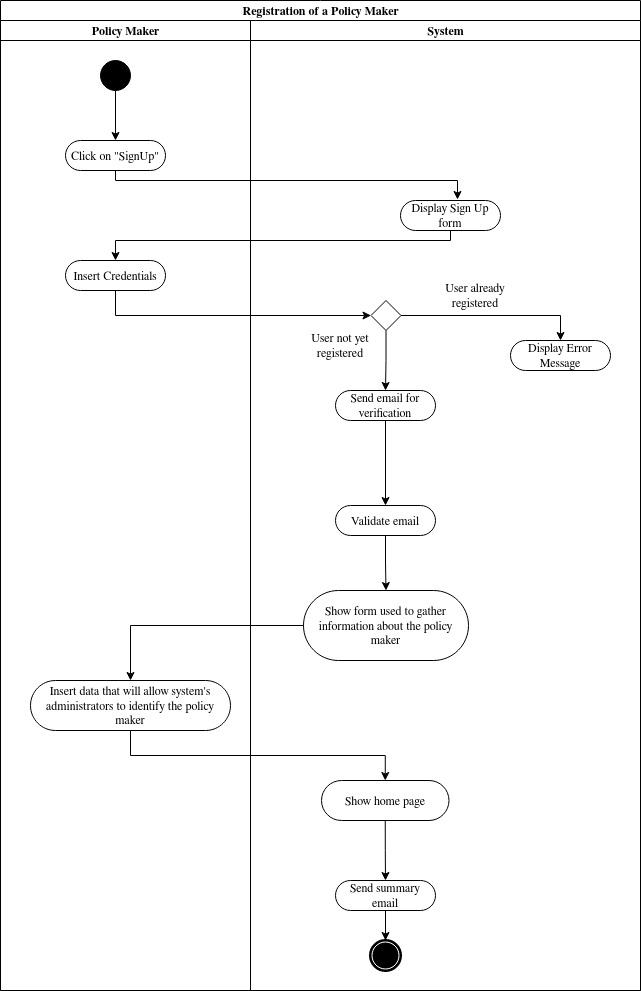
\includegraphics[width=250px]{ActivityDiagrams/PolicyMakerSignUp.jpg}
    \caption{Activity diagram: Policy Maker Sign Up}
\end{figure}
\subsubsection{Activity Diagram: User Login}
The following activity diagram describes the login process of the system. In particular, it maps the use case 0.1.
\begin{figure}[H]
    \centering
    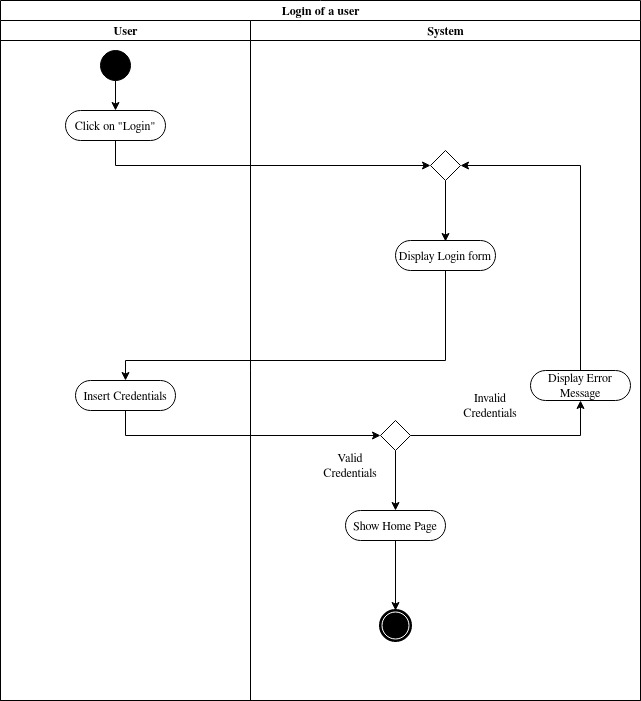
\includegraphics[width=250px]{ActivityDiagrams/UserLogin.jpg}
    \caption{Activity diagram: User Login}
\end{figure}
\subsubsection{Activity Diagram: Data Insertion}
The following activity diagrams describe how farmers and agronomists insert data inside the system. In particular, the two diagrams map the use cases 1.9 and 2.4 respectively.
\begin{figure}[H]
    \centering
    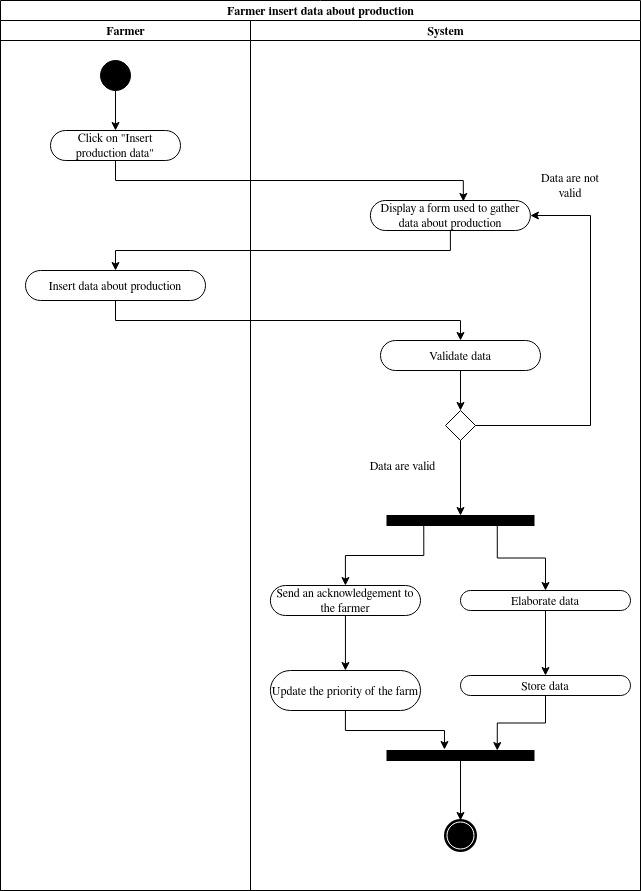
\includegraphics[width=250px]{ActivityDiagrams/FarmerInsert.jpg}
    \caption{Activity diagram: Farmer inserts data about the production}
\end{figure}
\begin{figure}[H]
    \centering
    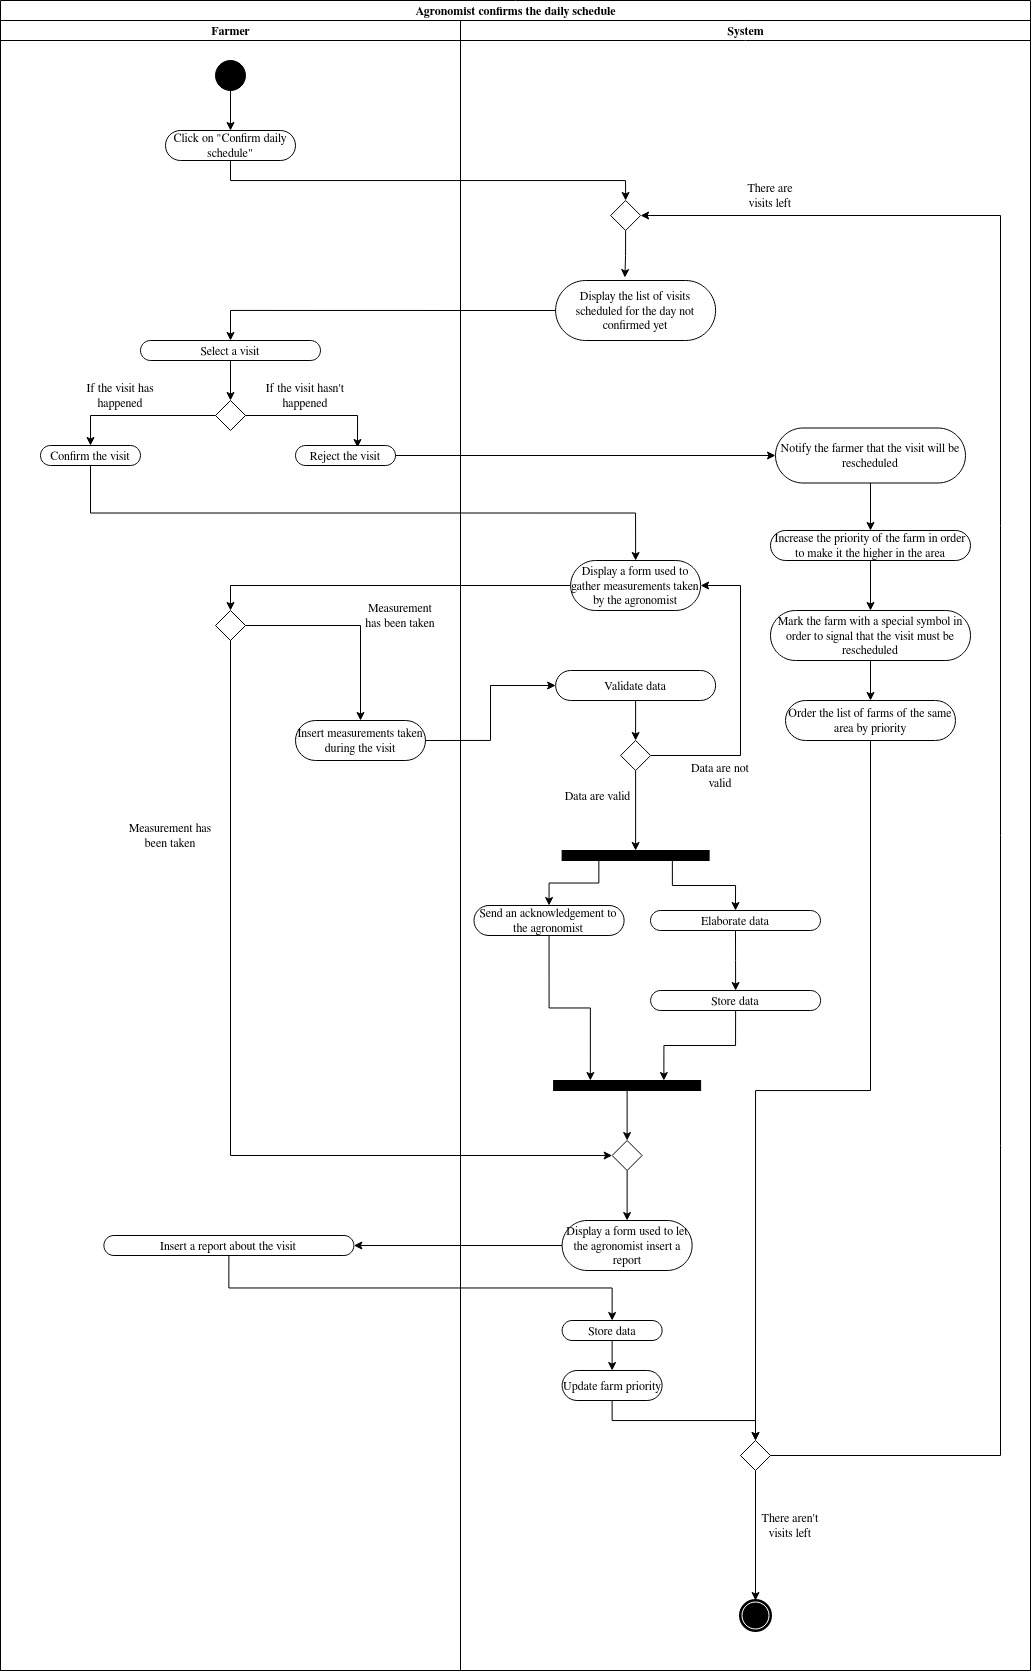
\includegraphics[width=350px]{ActivityDiagrams/AgronomistInsert.jpg}
    \caption{Activity diagram: Agronomist inserts data regarding a visit to a farm}
\end{figure}
\subsubsection{Activity Diagram: Visualize Data}
The following activity diagrams shows how users can visualize data of interest by using the system. In particular, the diagram maps the use case 0.2.
\begin{figure}[H]
    \centering
    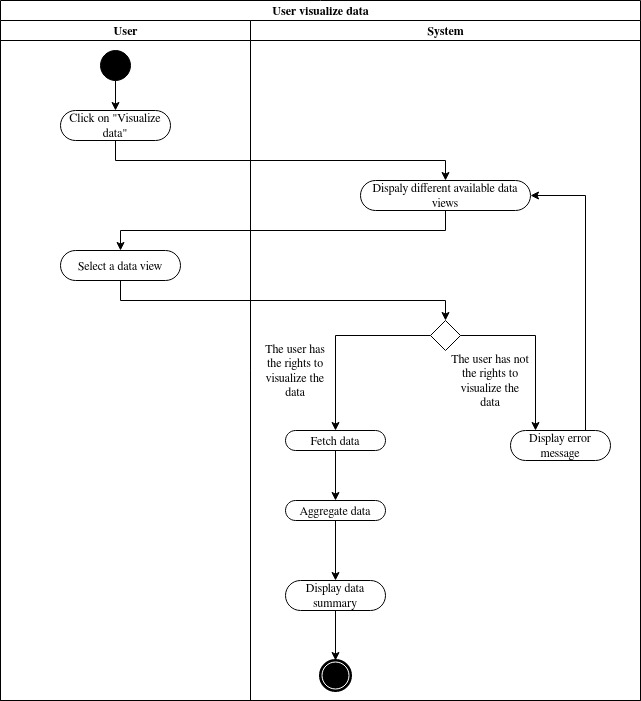
\includegraphics[width=250px]{ActivityDiagrams/VisualizeData.jpg}
    \caption{Activity diagram: User visualizes data summary}
\end{figure}
\subsubsection{Activity Diagram: Chat between agronomists and farmers}
The following activity diagram describes how agronomists and farmer can communicate by using the chat functionality offered by the system. In particular it maps the use cases 1.2, 2.2 and 1.6.
\begin{figure}[H]
    \centering
    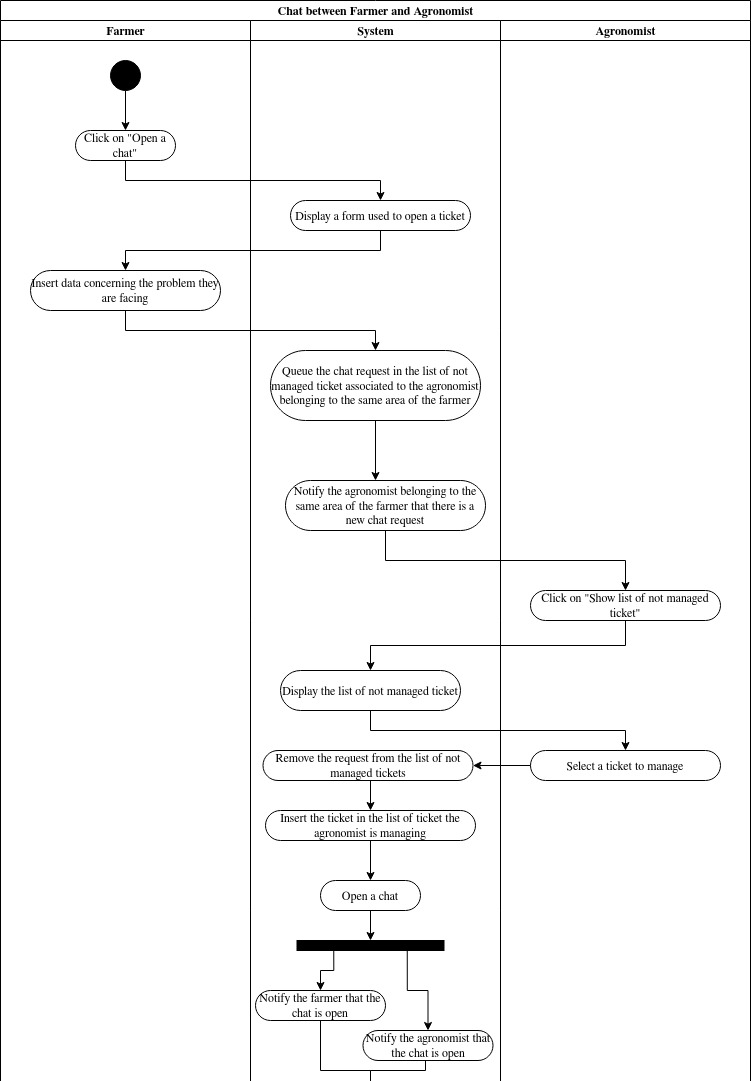
\includegraphics[width=300px]{ActivityDiagrams/Chat_1.png}
    \caption{Activity diagram: Chat between agronomists and farmers (part 1)}
\end{figure}
\begin{figure}[H]
    \centering
    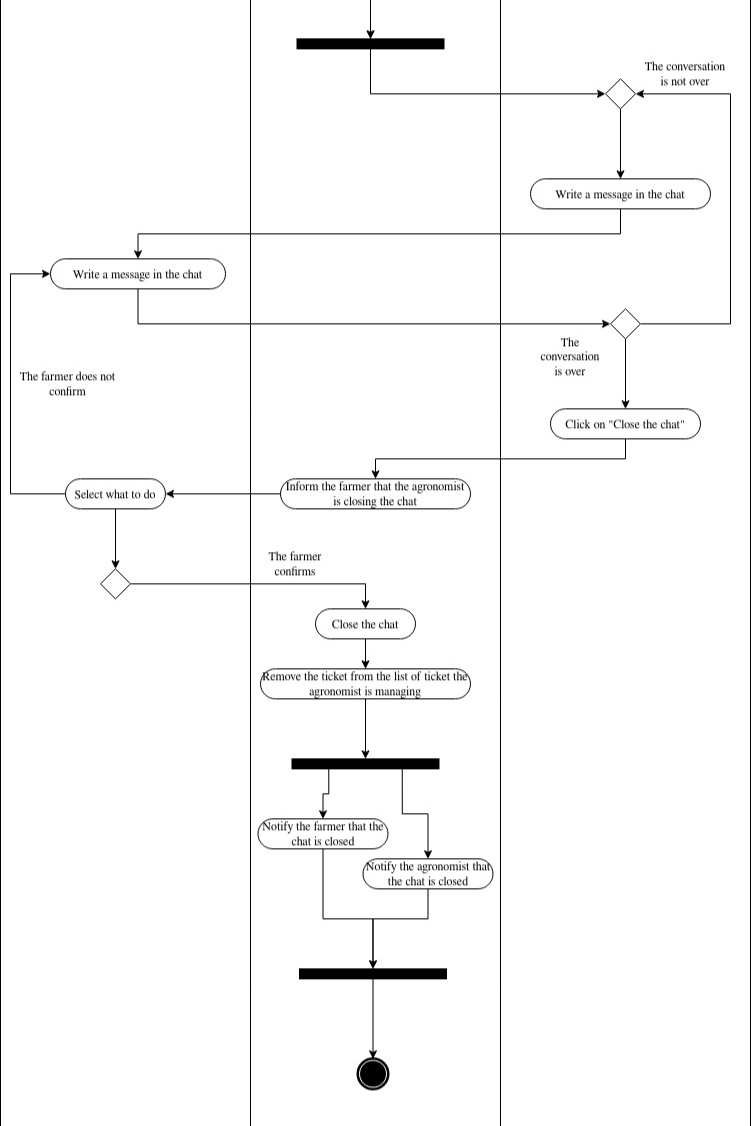
\includegraphics[width=300px]{ActivityDiagrams/Chat_2.png}
    \caption{Activity diagram: Chat between agronomists and farmers (part 2)}
\end{figure}
\subsubsection{Activity Diagram: Booking of  visit}
The following activity diagrams describes how a farmer can request a visit by an agronomist and how an agronomist can schedule a visit to a farm respectively. In particular the two diagrams map the use cases 1.3, 1.4, 1.5, 2.3 and 2.5.
\begin{figure}[H]
    \centering
    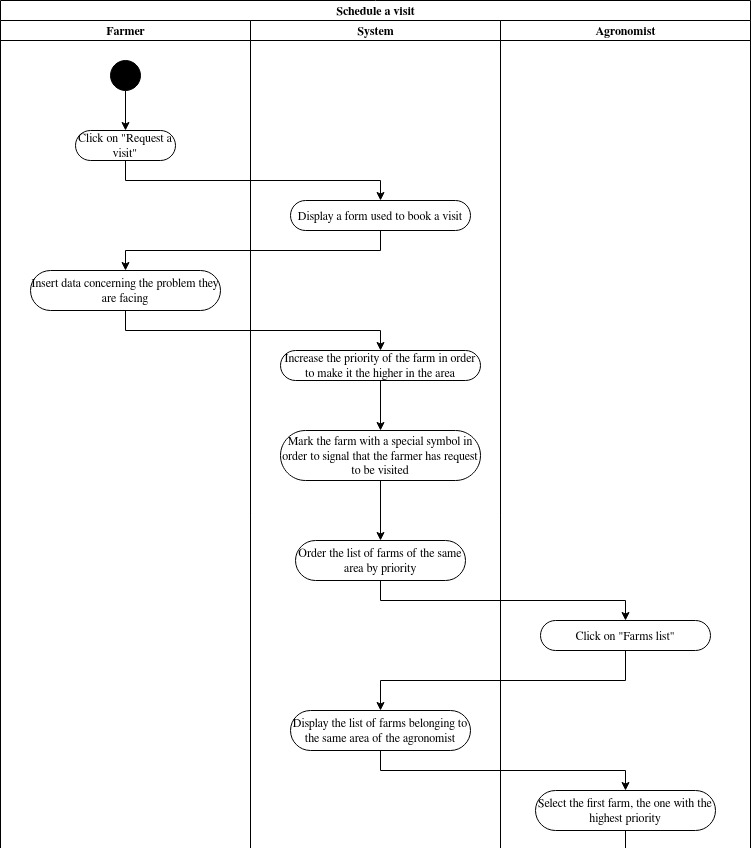
\includegraphics[width=300px]{ActivityDiagrams/BookingFromF_1.png}
    \caption{Activity diagram: Farmer requests a visit by an agronomist (Part 1)}
\end{figure}
\begin{figure}[H]
    \centering
    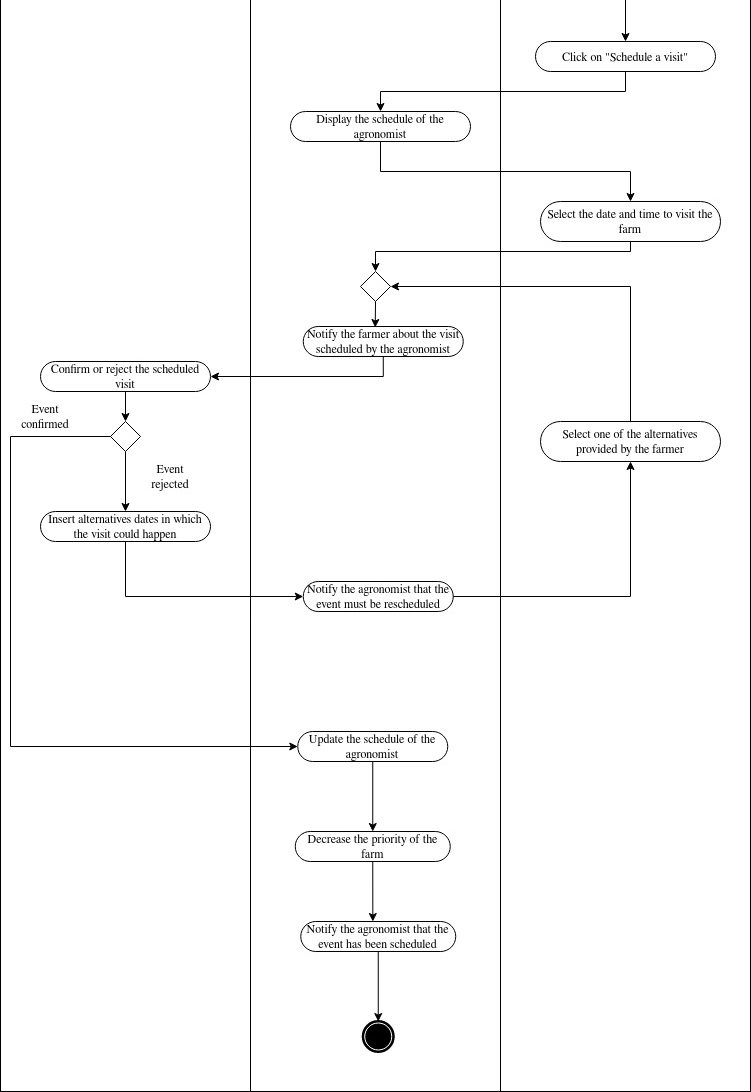
\includegraphics[width=300px]{ActivityDiagrams/BookingFromF_2.png}
    \caption{Activity diagram: Farmer requests a visit by an agronomist (Part 2)}
\end{figure}
\begin{figure}[H]
    \centering
    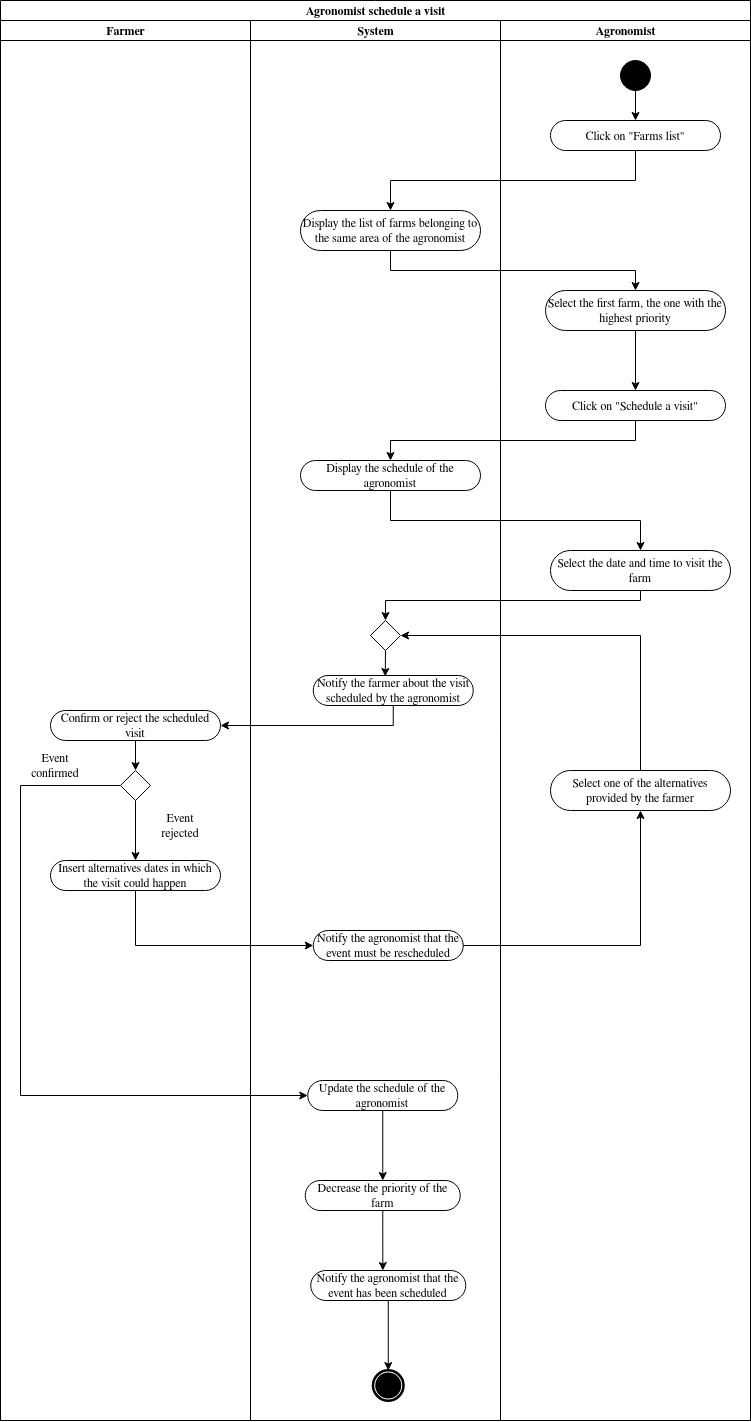
\includegraphics[width=300px]{ActivityDiagrams/BookingFromA.jpg}
    \caption{Activity diagram: Agronomist schedules a visit to a farm}
\end{figure}
\subsection{Mapping between Goals, Domain Assumptions and Requirements}
In the following will be shown which requirements and domain assumptions are needed ti fulfill each goals.\\


\textbf{G1 - Data Driven approach}
\begin{itemize}
    \item [$R01$] The system allows users to sign up
    \item [$R02$] Every user can access the system only if they are registered
    \item [$R03$] The system must allow to access the system only if the credentials used are correct
    \item [$R04$] The system must not allow to register two different users with the same username
    \item [$R05$] The system must not allow the same user to register themselves more than once
    \item [$R19$] The system must fetch data from different sources containing relevant information for the scope of the application
    \item [$R20$] The system must elaborate and aggregate data fetched from different sources
    \item [$D02$] Every user has an internet connection in order to interact with the system
    \item [$D03$] Every farmer has the capability to interact with the system
    \item [$D04$] Every agronomist has the capability to interact with the system
    \item [$D06$] Every farmer has an electronic device in order to interact with the system
    \item [$D07$] Every agronomist has an electronic device in order to interact with the system
    \item [$D09$] The farmers insert true and correct data about their production
    \item [$D10$] The agronomists insert true and correct data about measurements
    \item [$D15$] All those agronomist that take measurements do so in a consistent way
    \item [$D17$] Only real and capable agronomists are allowed to subscribe to the system
    \item [$D24$] External databases are correctly and periodically updated
\end{itemize}

\textbf{G2 - Help policy makers to implement better policies which will make Telangana’s agriculture better}
\begin{itemize}
    \item [$R01$] The system allows users to sign up
    \item [$R02$] Every user can access the system only if they are registered
    \item [$R03$] The system must allow to access the system only if the credentials used are correct
    \item [$R04$] The system must not allow to register two different users with the same username
    \item [$R05$] The system must not allow the same user to register themselves more than once
    \item [$R16$] The system allows the policy maker to see data about a specific farm
    \item [$R17$] The system allows the policy maker to see data about an area
    \item [$R18$] The system allows the policy maker to see data about all the areas in Telangana
    \item [$R19$] The system must fetch data from different sources containing relevant information for the scope of the application
    \item [$R20$] The system must elaborate and aggregate data fetched from different sources
    \item [$D02$] Every user has an internet connection in order to interact with the system
    \item [$D03$] Every farmer has the capability to interact with the system
    \item [$D04$] Every agronomist has the capability to interact with the system
    \item [$D05$] Every policy maker has the capability to interact with the system
    \item [$D06$] Every farmer has an electronic device in order to interact with the system
    \item [$D07$] Every agronomist has an electronic device in order to interact with the system
    \item [$D08$] Every policy maker has an electronic device in order to interact with the system
    \item [$D09$] The farmers insert true and correct data about their production
    \item [$D10$] The agronomists insert true and correct data about measurements
    \item [$D11$] The reports inserted by agronomists are sufficiently detailed
    \item [$D15$] All those agronomist that take measurements do so in a consistent way
    \item [$D18$] Only real and capable policy maker are allowed to subscribe to the system
    \item [$D22$] Every user has its own credentials
    \item [$D23$] The credentials used to access the system are not shareable
    \item [$D24$] External databases are correctly and periodically updated
\end{itemize}

\textbf{G3 - Help farmers to become weather resilient and increase their production}
\begin{itemize}
    \item [$R01$] The system allows users to sign up
    \item [$R02$] Every user can access the system only if they are registered
    \item [$R03$] The system must allow to access the system only if the credentials used are correct
    \item [$R04$] The system must not allow to register two different users with the same username
    \item [$R05$] The system must not allow the same user to register themselves more than once
    \item [$R10$] The system allows the farmer to see data about their farm
    \item [$R11$] The system must not allow the farmer to see data about farms other than theirs
    \item [$R19$] The system must fetch data from different sources containing relevant information for the scope of the application
    \item [$R20$] The system must elaborate and aggregate data fetched from different sources
    \item [$D02$] Every user has an internet connection in order to interact with the system
    \item [$D03$] Every farmer has the capability to interact with the system
    \item [$D04$] Every agronomist has the capability to interact with the system
    \item [$D06$] Every farmer has an electronic device in order to interact with the system
    \item [$D07$] Every agronomist has an electronic device in order to interact with the system
    \item [$D09$] The farmers insert true and correct data about their production
    \item [$D10$] The agronomists insert true and correct data about measurements
    \item [$D15$] All those agronomist that take measurements do so in a consistent way
    \item [$D16$] The farmers follows agronomist’s advice
    \item [$D17$] Only real and capable agronomists are allowed to subscribe to the system
    \item [$D20$] Each farmer’s account owns one and only one farm
    \item [$D21$] Each farm is owned by one and only one farmer
    \item [$D22$] Every user has its own credentials
    \item [$D23$] The credentials used to access the system are not shareable
    \item [$D24$] External databases are correctly and periodically updated
\end{itemize}

\textbf{G4 - Facilitate and make systematic the communication between farmers and agronomists}
\begin{itemize}
    \item [$R01$] The system allows users to sign up
    \item [$R02$] Every user can access the system only if they are registered
    \item [$R03$] The system must allow to access the system only if the credentials used are correct
    \item [$R04$] The system must not allow to register two different users with the same username
    \item [$R05$] The system must not allow the same user to register themselves more than once
    \item [$R06$] The system shall associate to each area one or more agronomists
    \item [$R07$] The system shall associate each farmer to one and only one area
    \item [$R08$] Each agronomist is associated to one and only one area
    \item [$R09$] The system allows the agronomist to see only the list of farms for which they are responsible of
    \item [$R10$] The system allows the farmer to see data about their farm
    \item [$R11$] The system must not allow the farmer to see data about farms other than theirs
    \item [$R12$] The system allows the agronomist to see data about a specific farm
    \item [$R13$] The system allows the agronomist to see data about the area for which they are responsible for
    \item [$R14$] The system must not allow the agronomist to see data about farms for which they are not responsible for
    \item [$R15$] The system must not allow the agronomist to see data about an area for which they are not responsible for
    \item [$R19$] The system must fetch data from different sources containing relevant information for the scope of the application
    \item [$R20$] The system must elaborate and aggregate data fetched from different sources
    \item [$R21$] The system allows farmers to request to have a chat with an agronomist
    \item [$R22$] The system allows agronomists to accept chat requests
    \item [$R23$] The system allows farmers and agronomists to interact through a chat
    \item [$R24$] A farmer, belonging to an area, can chat only with an agronomist belonging to the same area
    \item [$R25$] Each farmer can have at most one open chat at any given time
    \item [$R26$] Each agronomist can have multiple chats open at any given time
    \item [$R27$] The system allows only agronomists to close chats
    \item [$R28$] The system allows farmers to request a visit from an agronomist
    \item [$R29$] The system must show an agronomist a list of farms they have to visit, ordering them by priority
    \item [$R30$] The system must prioritize the farms that need help
    \item [$R31$] The agronomist must prioritize the farms that the system prioritize
    \item [$R32$] The system allows agronomists to schedule a visit at any farm of their competence
    \item [$R33$] The system allows agronomist to set up a daily schedule
    \item [$R34$] The system must notify a farmer when an agronomist schedules a visit to their farm
    \item [$R35$] The system must notify an agronomist when a farmers cancels a scheduled visit to their farm
    \item [$R36$] The system must notify a farmer when an agronomist cancels a scheduled visit to their farm
    \item [$R37$] The system allows agronomists to cancel a scheduled visits within one day before
    \item [$D01$] There are enough agronomists for each area
    \item [$D02$] Every user has an internet connection in order to interact with the system
    \item [$D03$] Every farmer has the capability to interact with the system
    \item [$D04$] Every agronomist has the capability to interact with the system
    \item [$D06$] Every farmer has an electronic device in order to interact with the system
    \item [$D07$] Every agronomist has an electronic device in order to interact with the system
    \item [$D09$] The farmers insert true and correct data about their production
    \item [$D10$] The agronomists insert true and correct data about measurements
    \item [$D12$] The agronomists always confirms all the visits that they have done, sooner or later
    \item [$D13$] A visit in an agronomist schedule is confirmed only if it is actually done by the agronomist
    \item [$D14$] All the agronomists have at least decent capabilities of managing and organizing their own schedule
    \item [$D15$] All those agronomist that take measurements do so in a consistent way
    \item [$D16$] The farmers follows agronomist’s advice
    \item [$D17$] Only real and capable agronomists are allowed to subscribe to the system
    \item [$D19$] The agronomist that wants to visit a farm will reach an agreement with the owner farmer on the day and date of the appointment within about 14 days from the first appointment request
    \item [$D20$] Each farmer’s account owns one and only one farm
    \item [$D21$] Each farm is owned by one and only one farmer
    \item [$D22$] Every user has its own credentials
    \item [$D23$] The credentials used to access the system are not shareable
    \item [$D24$] External databases are correctly and periodically updated
\end{itemize}

\textbf{G5 - Create a network of farmers}
\begin{itemize}
    \item [$R01$] The system allows users to sign up
    \item [$R02$] Every user can access the system only if they are registered
    \item [$R03$] The system must allow to access the system only if the credentials used are correct
    \item [$R04$] The system must not allow to register two different users with the same username
    \item [$R05$] The system must not allow the same user to register themselves more than once
    \item [$R38$] The system shall allow farmers to interact through a forum with other farmers and agronomists
    \item [$R39$] The system shall allow agronomists to interact through a forum with other agronomists and farmers
    \item [$R40$] The forum allow to each farmer or agronomist with each other no matter the area they belong to
    \item [$D02$] Every user has an internet connection in order to interact with the system
    \item [$D03$] Every farmer has the capability to interact with the system
    \item [$D04$] Every agronomist has the capability to interact with the system
    \item [$D06$] Every farmer has an electronic device in order to interact with the system
    \item [$D07$] Every agronomist has an electronic device in order to interact with the system
    \item [$D22$] Every user has its own credentials
    \item [$D23$] The credentials used to access the system are not shareable
\end{itemize}
\section{Performance requirements}
The response time is not the main focus of our system. In fact, scalability surely has more impact in the system: we need to support a lot of different areas in Telangana, which include several farmers and agronomists. Furthermore, in the future the system may be adopted by more regions of India, and even by different countries. 
The system must be able to process a large amount of data, including data fetched periodically from different external databases that will be elaborated in real-time, allowing users to access it.
\section{Design constraints}
\subsection{Standard compliance}
The system described will be used by the government, therefore it must be compliant with the Digital Public Goods (DPG) standard.\\
The Digital Public Goods Standard is a set of specifications and guidelines designed to maximise consensus about whether a digital solution conforms to the definition of a digital public good: open-source software, open data, open AI models, open standards, and open content that adhere to privacy and other applicable best practices, do no harm by design and are of high relevance for attainment of the United Nations 2030 Sustainable Development Goals (SDGs).\\ \\
More information can be found here: https://digitalpublicgoods.net/standard/
\subsection{Hardware Constraints}
Each person interested in using the system described in this document must have a device connected to the Internet, which could be a smartphone, a tablet or a personal computer. In particular, the basic requirement is to have an Internet browser installed on the device. There is then the possibility of downloading and installing the official DREAM application from the most important stores, such as \emph{Apple’s App Store} or \emph{Google’s Play Store} or \emph{Huawei's AppGallery}.
\section{Software system attributes}
\subsection{Reliability}
The system must prevent downtime. In fact, agronomists' work depend on the functioning of the system, and any downtime could make the schedule of each agronomist shift or could prevent users to insert useful data in the system.
\subsection{Availability}
The system must be available as much as possible. In fact, because the system could be adopted worldwide, and therefore could be used in different time zones, the system must be available 24 hours per day every day of the year.
\subsection{Security}
Communication between parties are encrypted and goes on a secure channel (through SSL protocol). Furthermore, the database guarantees that performed operations are always authorized.
\subsection{Maintainability}
The system must be designed in such a way that permits future addition of functionalities with minimum effort. For example, new machine learning modules could be needed in the future as long as agriculture techniques evolve. Moreover, the rising of 5G could allow the adoption of more complex sensors systems that could be included in the system.
\subsection{Portability}
The system must be supported on the principal operating systems, either mobile and computers. It is in any case usable on every web browser, from every device.
\subsection{Scalability}
The scalability of the system must be an absolute priority. In fact, in the future the system may be adopted by more regions of India other than Telangana, and even by more states spread around the world.
\subsection{Usability}
The system should be very easy to use and intuitive. Indeed, potentially, it could be used by a large spectrum of people (e.g. from farmers to policy makers) having different backgrounds and educations.
\chapter{Formal analysis using Alloy}
We want to formalize our application by creating a model with Alloy. For this reason, we describe what are the main topics that we want to address in the formal analysis:

\begin{itemize}
  \item Farmers and Agronomists are organized into geographical areas. We want to prove that they can interact with each other, through different mechanisms, only if they belong to the same area
  \item Each Agronomist has a schedule of visits to the farms: when a schedule is confirmed and inserted into the system they must insert a report about the visits they have done
  \item The policy makers must see everything that allows them to understand how both the farmers and the agronomists are performing. We will show that they are able to see data about production of the farms along with report generated by the agronomists
\end{itemize}
\section{Alloy Code}
\lstinputlisting[language=alloy]{Code/dreamv3_formatted.als}
\section{Alloy Worlds}
\subsection{Farmer requests a chat with an Agronomist}
\begin{figure}[H]
    \centering
    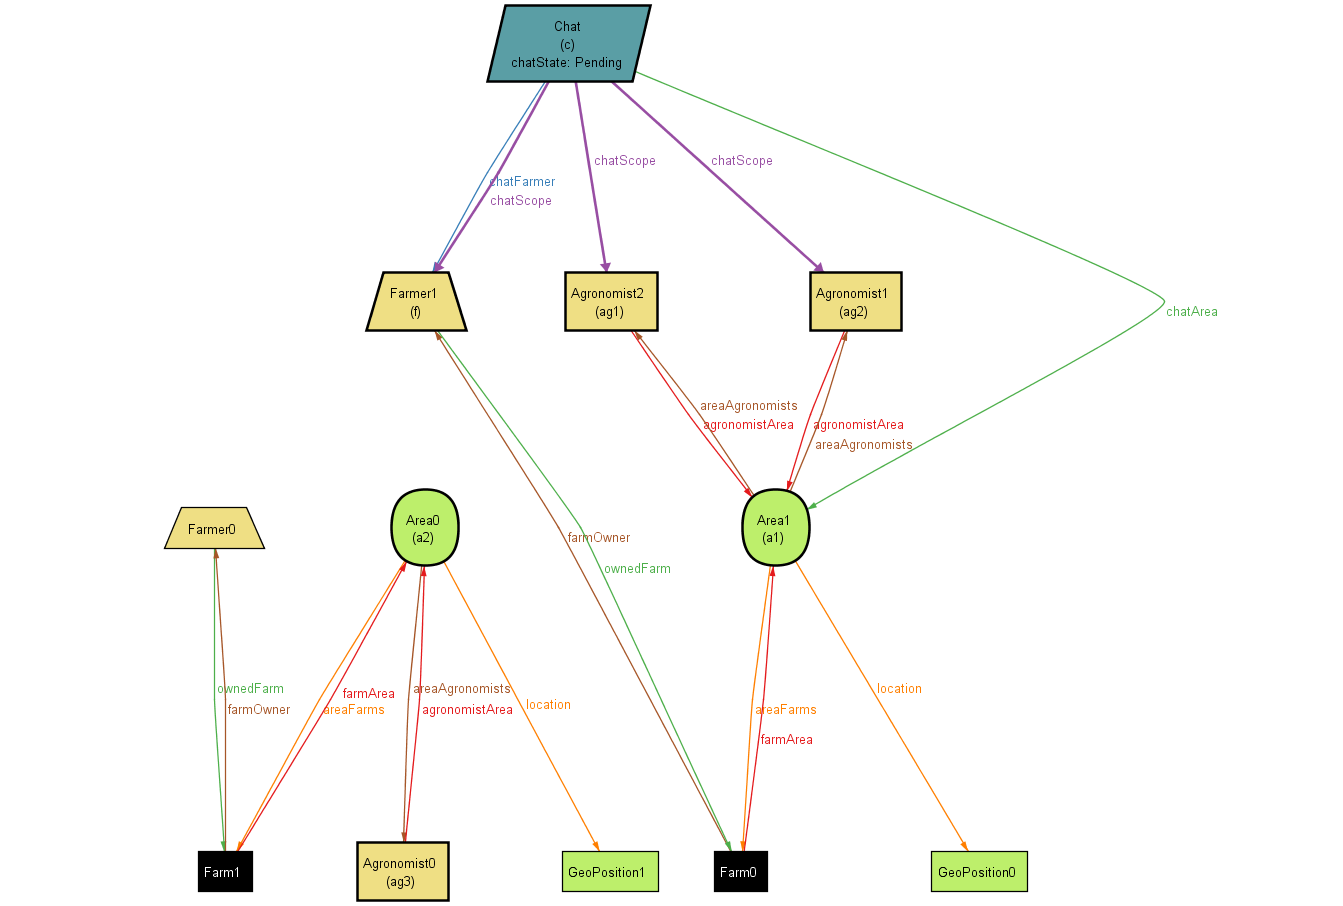
\includegraphics[width=450px]{Alloy/chatPending.png}
    \caption{pred chatPending}
\end{figure}
This diagram shows a Farmer (f) that has opened a chat (c). The just opened chat is in state “pending” meaning that no Agronomists took it yet. There are two Agronomists (ag1,ag2) that belong to the same area (a1) of the Farmer’s farm. Furthermore, there is another area (a2) and another Agronomist (ag3) in this model. As we can see the chat scope is correctly related only to ag1 and ag2. On the other hand, ag3 that belongs to a different area, a2, cannot see the pending chat.
\subsection{Agronomist schedule a visit to a Farm}
\begin{figure}[H]
    \centering
    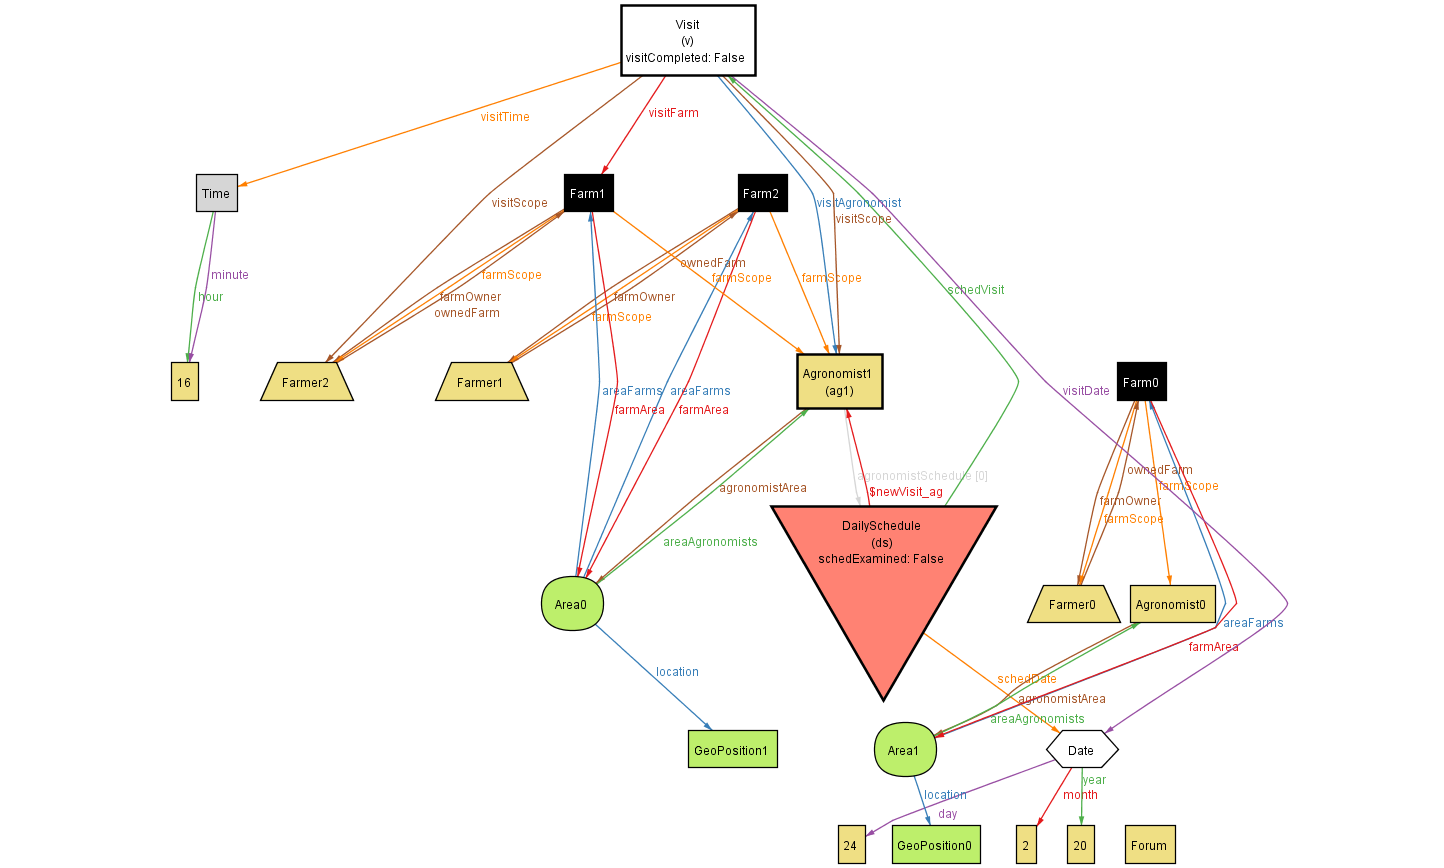
\includegraphics[width=450px]{Alloy/newVisit.png}
    \caption{pred newVisit}
\end{figure}
The diagram shows that the Agronomist (ag1) has updated one of their daily schedules to take into account a new visit (v). The visit is set to be to Farm1, that belongs to Area0, the same of the Agronomist (ag1). We can notice that in this instance of our model, there is another area, Area1, that is completely separated from Area0. In fact, ag1 can see Farm1 and Farm2, not Farm0. Furthermore, we can notice how Farmer2, which is the owner of the Farm1, the one that is addressed in the new visit (v), can see it; Farmer0 and Farmer1 instead, do not have the appropriate visitScope relation.
\subsection{Agronomist confirms and inserts a daily schedule into the system}
\begin{figure}[H]
    \centering
    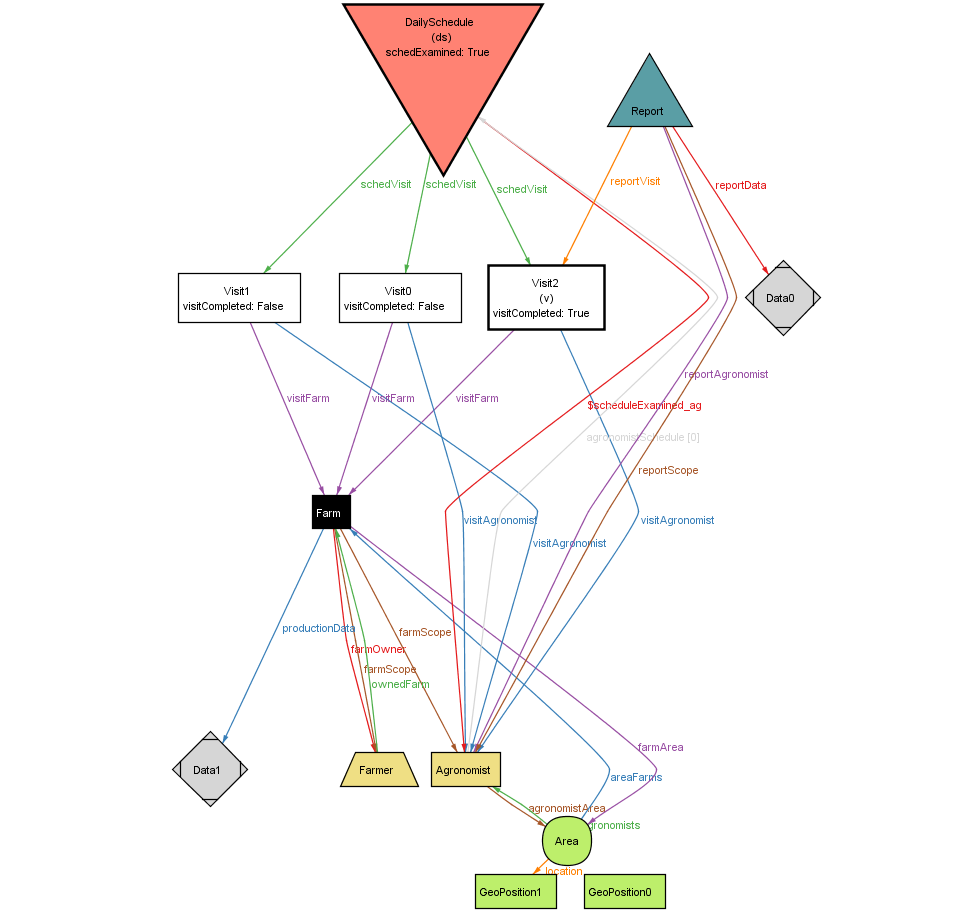
\includegraphics[width=450px]{Alloy/scheduleExamined.png}
    \caption{pred scheduleExamined}
\end{figure}
The diagram shows that the Agronomist present has a DailySchedule (ds) which has been “examined”. It means that the Agronomist has confirmed and inserted the daily schedule into the system. As we can see, since the daily schedule (ds) has a visit that was completed, the Agronomist has also produced a Report of such visit (v). Notice that, since Visit0 and Visit1 were not completed, even if the schedule was confirmed no associated reports have been produced.

\subsection{An interesting and general instance of the model}
\begin{figure}[H]
    \centering
    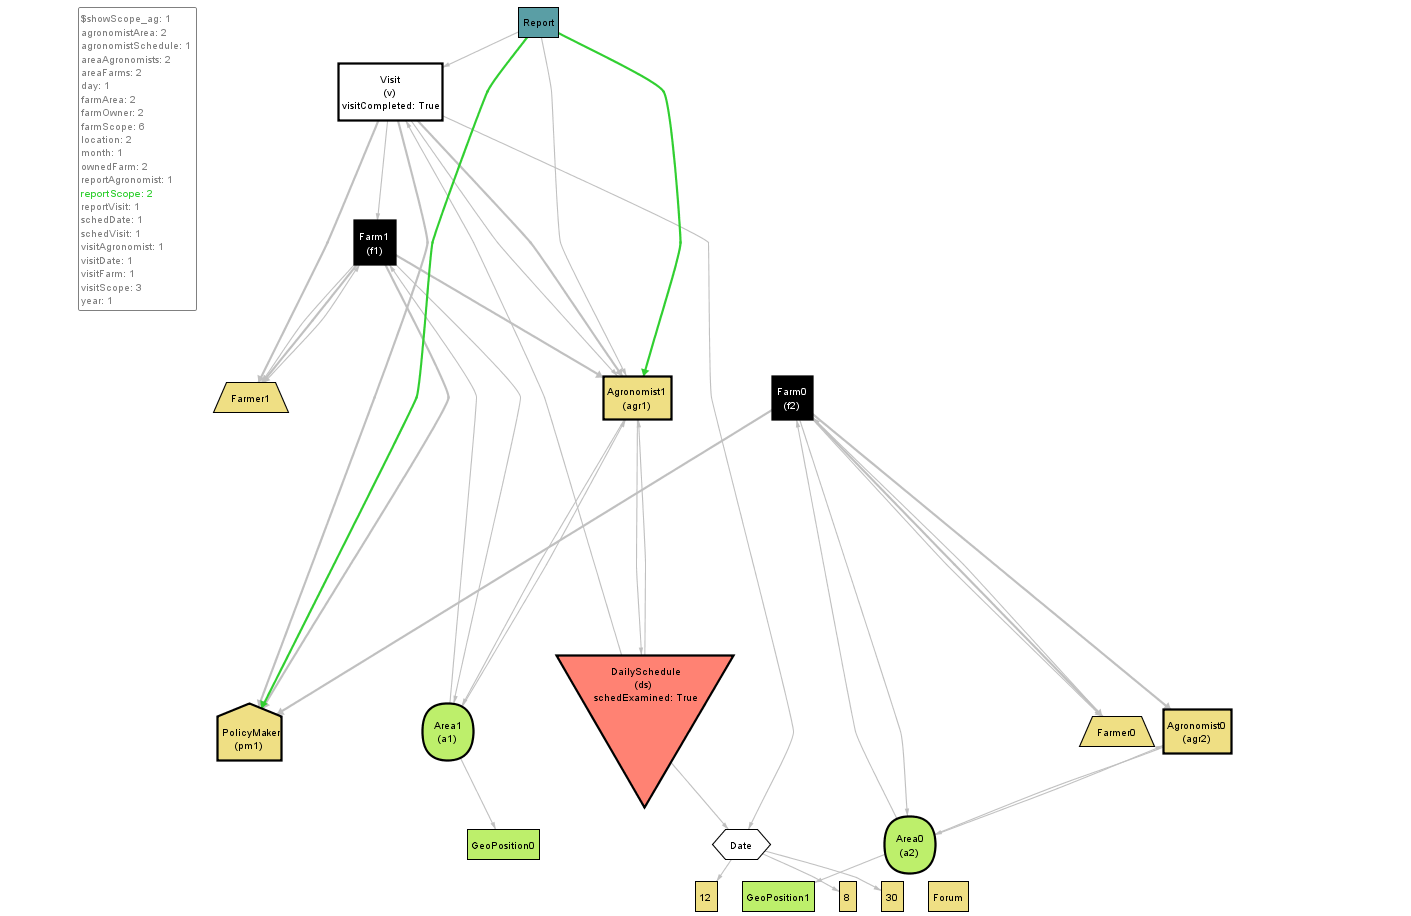
\includegraphics[width=450px]{Alloy/reportScope.png}
    \caption{pred showScope Report}
\end{figure}
In this instance we have an Agronomist (ag1) that has produced a report of a visit (v). As we can see from the green arrows, the report is visible to (ag1) that produced it, and to the policy maker that is present in this instance (pm1).

\begin{figure}[H]
    \centering
    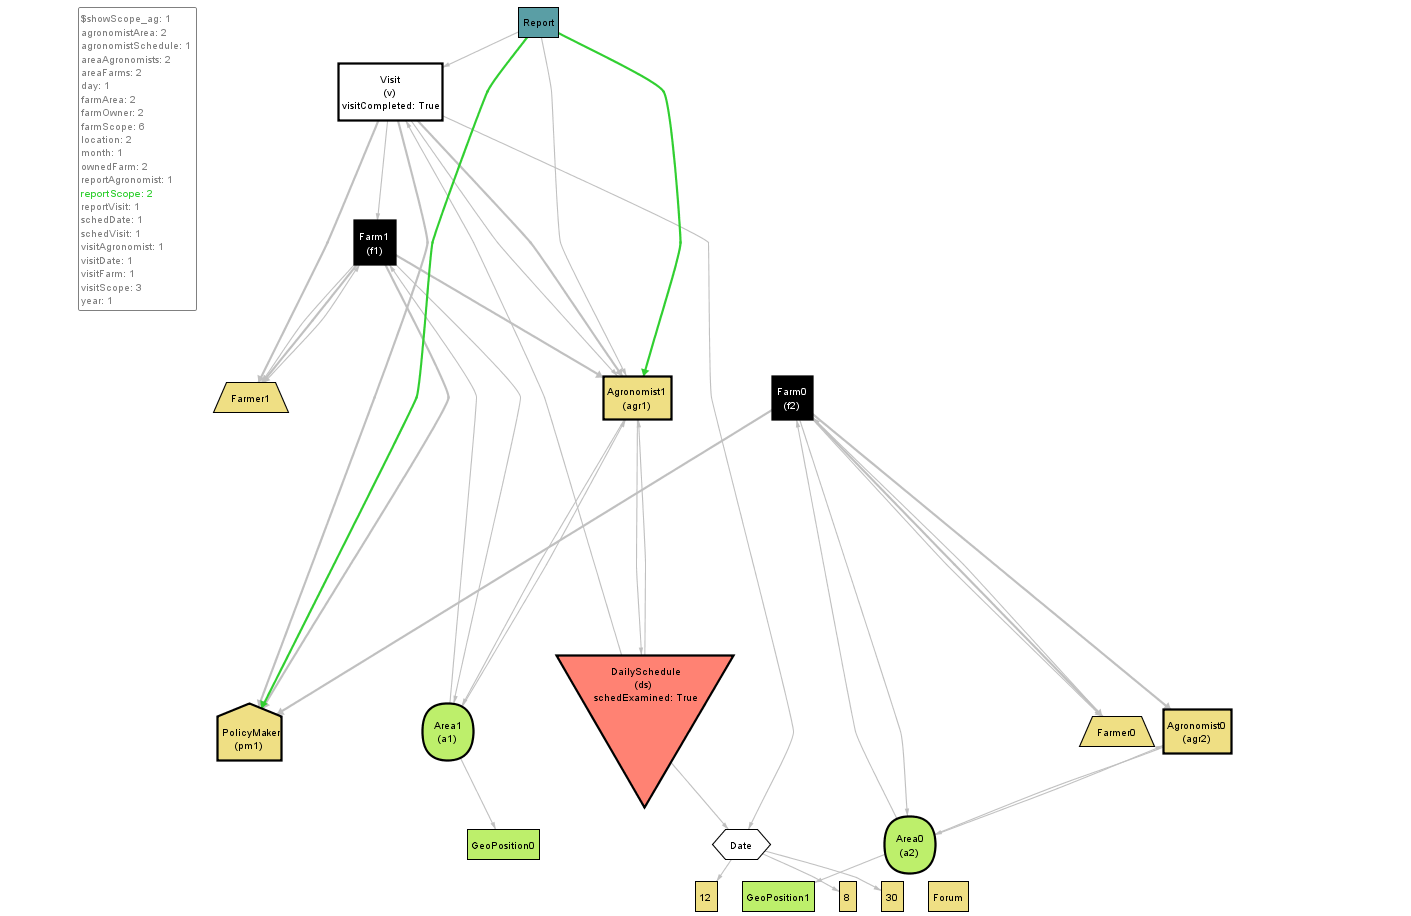
\includegraphics[width=450px]{Alloy/reportScope.png}
    \caption{pred showScope Farm}
\end{figure}
The light red arrows instead specify the visibility of the Farms: while for the farmers and the agronomist the visibility is limited with respect to the area of belonging, the Policy Maker (pm1) can see both of the farms present, independently from their area. 

\begin{figure}[H]
    \centering
    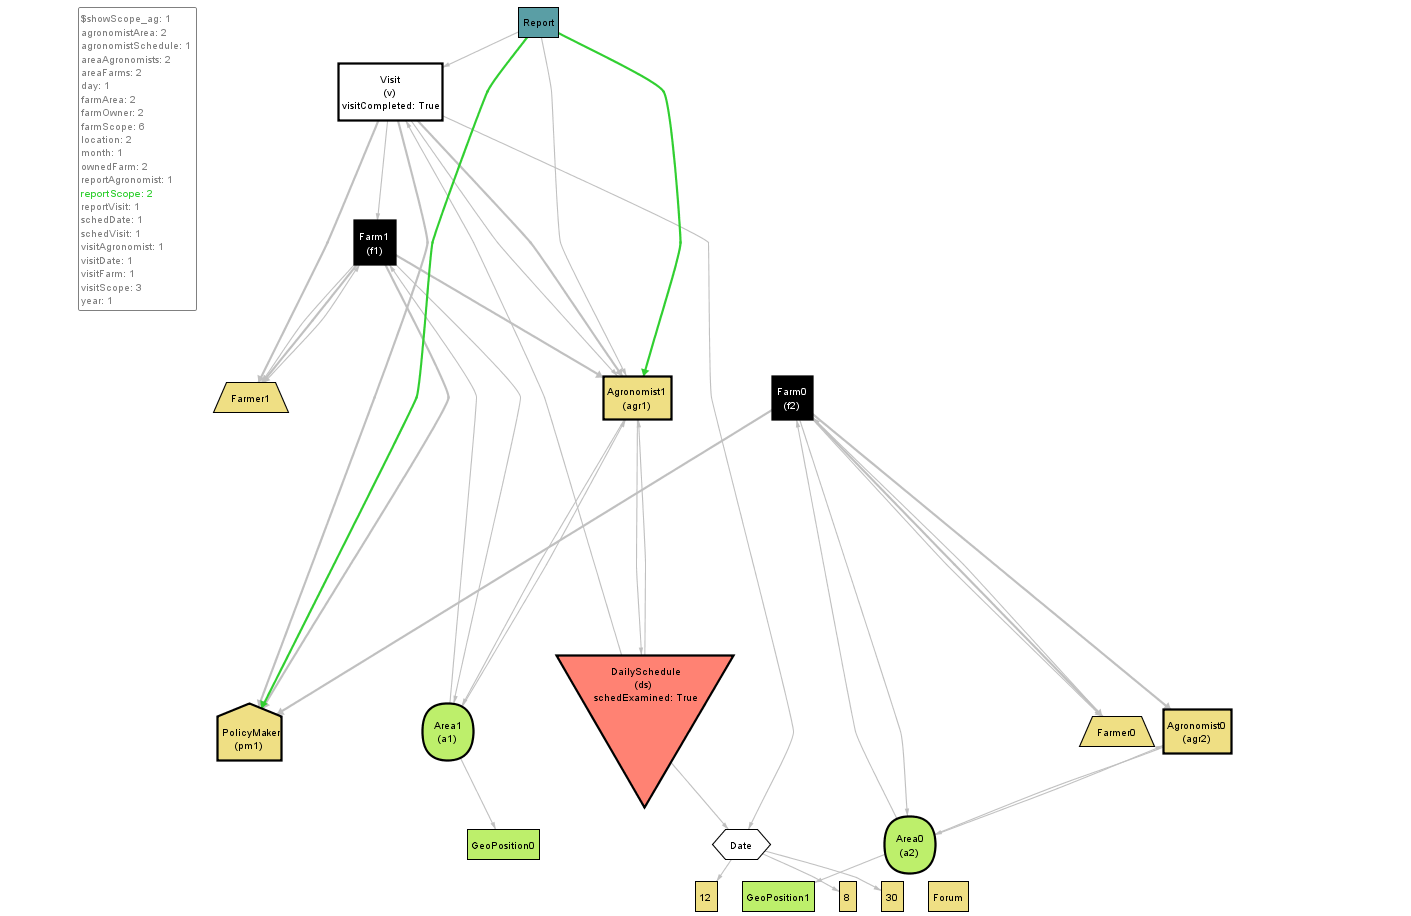
\includegraphics[width=450px]{Alloy/reportScope.png}
    \caption{pred showScope Visit}
\end{figure}
The yellow arrows specify the visibility of the visit, completed, (v). Thus, we can see, differently from the previous diagram (4.2.2) that here there is also a Policy Maker (pm1) that can see the visit (v).
\chapter{Effort spent}
\begin{table}[H]
\centering
\begin{tabular}{|l|l|}
\hline
\textbf{Student}       & \textbf{Effort} \\ \hline
Salvatore Maccarrone   & 55h             \\ \hline
Massimiliano Pellizzer & 55h             \\ \hline
Andrea Prati           & 55h             \\ \hline
\end{tabular}
\end{table}
\section{Thought process}
The drafting process of this document started on October 20,  we had a few meetings where we read and tried to figure out the most important goals of the assignment.\\ We started writing down the phenomena and the Domain Assumption, then we wrote the requirements.\\
At this point we divided the sections of the document in order to work in parallel and try to avoid any kinds of ambiguity, actually we used an iterative writing process, everyone put something of their personal thoughts in each section, always keeping the whole document consistent as much as possible. \\
The sections have not been written in the order they appear in the last version of the document.
\subsection{Comments about the assignment}
The assignment was described with a certain level of ambiguity, thus we had to make some decisions that weren’t specified in it. \\We interpreted the assignment as a request to design a platform that should be a reference for all the Telangana’s Farmers, Agronomists and Policy Makers, always considering that the system needs to have a strong Data Driven nature.  \\
Therefore, we wrote a first version of DREAM, a platform that can be divided into three categories: Data, Community and Management. More details about these categories are written in the Section 1.2 of the document. \\

We started thinking about which data would have been produced through DREAM and which data would have been taken from external DBs. \\
Then we started designing the communication channels which would have allowed the users to talk with each other. Here we started to think about the Forum and the chat mechanism.\\
After having a first idea about the community, we thought about how the Agronomist and the Policy Maker would have been able to use the data stored into the system, and properly processed and aggregated, in order to acquire information about the live status of the farms on the territory. \\
As last thing we decided the method to use to keep track of the steering initiatives given to the farmers by the agronomists. \\

The interview with the stakeholders (the Q\&A) was useful in order to have a better idea about the domain. Indeed, during this event the farmer’s average digital competence was clarified, we discovered that in India most of the farmers have a basic digital competence, that is why we decided to assign them just the insertion about their harvests and the community features.\\

Ultimately, as requested by the stakeholders, we designed DREAM first and foremost as a platform, to which all the desired analytics can then be associated.\\

Looking at the GitHub repository that we listed among the references, we find in the README.md in the root of the repository an image that describes the data flow of the system: \href{https://user-images.githubusercontent.com/42402451/138163914-85322590-f0ea-44f4-88e6-4452f49d7057.png}{link}. \\
We have used that  image as a reference, but we have only considered the application aspect of that schema.\\
In addition, in the top left corner we find the merge into a single cloud data storage of some data, this aspect has not been described in this document because, from the interview with the stakeholders we considered more important to stress the nature of the platform itself, in particular, we note that we were told this: \\
“Please assume all data to be as the datasets that are given and available to you. \\The data
processing and analytics should not be the focus of the work; rather, the DREAM platform and its elaboration should be the major focus, perhaps designing in sight of specifying further analytics around what we discussed together and what is documented in the specifications given.”
\subsection{Trackability of the writing process}
We worked approximately at least half of the hours reported in section 5 remotely, using the Google suite. The document named "RASD\textunderscore ALPHA" is the one that we considered to be almost as the official document: that is why we will report a link to it in the github repo. \\
We expect it to be useful to understand how the various sections of the final document have been produced and organized together. In fact, often the different sections of the document were written using different google documents, so that we could focus better on individual sections and facilitate the work of comparing the cohesion and coherence of the document.
\end{document}
